\documentclass[leqno]{scrartcl}
\usepackage[utf8]{inputenc}
\usepackage[english]{babel}

% Standard American Math Society packages provide theorem environments, symbols,
% etc.
\usepackage{amsmath, amsfonts, amsthm}
\usepackage{amssymb}
\usepackage{mathrsfs}
\usepackage{mathtools}

\usepackage{enumitem}

% For including graphics (such as charts and diagrams.)
\usepackage{graphicx}
\graphicspath{ {.} }
\usepackage{tikz-cd}
\usetikzlibrary{shapes,arrows}

% Allows customizing section commands
\usepackage{sectsty}
% Make all sections centered, the default font and small caps
\allsectionsfont{\normalfont\textbf}

% Custom headers and footers
\usepackage{fancyhdr}
% Makes all pages in the document conform to the custom headers and footers
\pagestyle{fancyplain}
% No page header - if you want one, create it in the same way as the footers
% below
\fancyhead{}
% Empty left footer
\fancyfoot[L]{}
% Empty center footer
\fancyfoot[C]{}
% Page numbering for right footer
\fancyfoot[R]{\thepage}
% Remove header underlines
\renewcommand{\headrulewidth}{0pt}
% Remove footer underlines
\renewcommand{\footrulewidth}{0pt}
% Customize the height of the header
\setlength{\headheight}{13.6pt}

% Number equations within sections
% (i.e. 1.1, 1.2, 2.1, 2.2 instead of 1, 2, 3, 4)
\numberwithin{equation}{section}
% Number figures within sections
% (i.e. 1.1, 1.2, 2.1, 2.2 instead of 1, 2, 3, 4)
\numberwithin{figure}{section}
% Number tables within sections
% (i.e. 1.1, 1.2, 2.1, 2.2 instead of 1, 2, 3, 4)
\numberwithin{table}{section}

% Removes all indentation from paragraphs - comment this line for an
% assignment with lots of text
\setlength\parindent{0pt}
\setlength{\parskip}{0.5em}


% The chngcntr ("change counter") package is used here so that subsection
% numbers are written without the leading section number. This takes place in
% the subsection headings as well as the theorem environment numbering.
%
% Before:
% 1. Section
% 1.1. Subsection
% Problem 1.1.1. What is 1 + 1?
% Problem 1.1.2. What is 1 + 2?
%
% After:
% 1. Section
% 1. Subsection
% Problem 1.1. What is 1 + 1?
% Problem 1.2. What is 1 + 2?
\usepackage{chngcntr}
\counterwithout{subsection}{section}

% The problem environment is a regular ams theorem environment with "Problem"
% text and some leading space to give some separation between the problems.
\theoremstyle{definition}
\newtheorem{problem-internal}{}[subsection]
\newenvironment{problem}{
	\medskip
	\begin{problem-internal}
	}{
\end{problem-internal}
}

% The solution environment is a proof environment with the "solution" text as
% well as the following adjustments:
% - No indent on paragraphs;
% - A small amount of space between paragraphs.
%
% Note: The negative space at the beginning is to remove the space before the
% first paragraph in the solution.
\newenvironment{solution}{
	\begin{proof}[Solution]
		\vspace{-8px}
		\setlength{\parskip}{4px}
		\setlength{\parindent}{0px}
	}{
\end{proof}
}

% Proposition environment for formatting some problems.
\theoremstyle{theorem}
\newtheorem*{proposition}{Proposition}

% Renewing the \thesection command changes the section numbers to roman
% numerals. This matches the style of the Aluffi textbook.
%
% Before:
% 1. Section
% 1.1. Subsection
%
% After:
% I. Section
% I.1. Subsection
\renewcommand{\thesection}{\Roman{section}} 

% Renewing the \qedsymbol command changes the QED symbol. This QED symbol is
% automatically used by the proof environment.

% Set with spacing padding for the curly braces.
\newcommand{\set}[1]{\left\{\,#1\,\right\}}

\newcommand{\id}{\mathrm{id}}
\DeclareMathOperator{\im}{im}
\DeclareMathOperator{\coker}{coker}
\DeclareMathOperator{\stab}{Stab}
\DeclareMathOperator{\spec}{Spec}
\newcommand{\pset}{\mathscr{P}}
\newcommand{\Obj}{\mathrm{Obj}}
\newcommand{\Hom}{\mathrm{Hom}}
\newcommand{\End}{\mathrm{End}}
\newcommand{\Aut}{\mathrm{Aut}}
\newcommand{\Inn}{\mathrm{Inn}}
\newcommand{\abs}[1]{\left|#1\right|}
\newcommand{\norm}[1]{\left|\left|#1\right|\right|}
% Inuitive "from" command draws an arrow pointing left, A <- B reads "A from p"
\newcommand{\from}{\leftarrow}
\newcommand{\quotuniv}[1]{\overline{#1}}

% Commands for some frequently used categories.
\newcommand{\C}{\mathsf{C}}
\newcommand{\Cop}{\mathsf{C^{op}}}
\newcommand{\Cset}{\mathsf{Set}}
\newcommand{\Cgrp}{\mathsf{Grp}}
\newcommand{\Cab}{\mathsf{Ab}}
\newcommand{\CGset}{\ensuremath{G\text{-}\Cset}}
\newcommand{\Cring}{\ensuremath{\mathsf{Ring}}}
\newcommand{\CRmod}{\ensuremath{R\text{-}\mathsf{Mod}}}
\newcommand{\CRalg}{\ensuremath{R\text{-}\mathsf{Alg}}}

% Frequently used sets.
\newcommand{\N}{\mathbb{N}}
\newcommand{\Zs}{\mathbb{Z}}
\newcommand{\Qs}{\mathbb{Q}}
\newcommand{\R}{\mathbb{R}}
\newcommand{\Cs}{\mathbb{C}}
\newcommand{\Hs}{\mathbb{H}}

% Matrices.
\newcommand{\mM}{\mathcal{M}}
\newcommand{\mGL}{\mathrm{GL}}
\newcommand{\mSL}{\mathrm{SL}}
\newcommand{\mPSL}{\mathrm{PSL}}
\newcommand{\mO}{\mathrm{O}}
\newcommand{\mSO}{\mathrm{SO}}
\newcommand{\mU}{\mathrm{U}}
\newcommand{\mSU}{\mathrm{SU}}
\newcommand{\mgl}{\mathfrak{gl}}
\newcommand{\msl}{\mathfrak{sl}}
\newcommand{\mso}{\mathfrak{so}}
\newcommand{\msu}{\mathfrak{su}}

% Frequently used groups.
\newcommand{\Z}[1]{\mathbb{Z}/#1\mathbb{Z}}
\newcommand{\gen}[1]{\ensuremath{\langle #1 \rangle}}

% Operators.
\DeclareMathOperator{\lcm}{lcm}
\DeclareMathOperator{\tr}{tr}

% Vectors.
\renewcommand{\vec}[1]{\mathbf{#1}}

\begin{document}
	
\section{Preliminaries: Set theory and categories}
\setcounter{subsection}{2}

\subsection{Category Theory}

% Problem 3.1
\begin{problem}
\end{problem}

\begin{solution}
	To make this into a category, we have to define the composition set-function $\circ_{Cop} : \Hom_{\Cop}(A,B) \times \Hom_{\Cop}(B,C) \to \Hom_{\Cop}(A,C)$, for $A,B,C$ objects of $\Cop$. Let $f \in \Hom_{\Cop}(A,B)$ and $g \in \Hom_{\Cop}(B,C)$ be morphisms in $\Cop$. We will define the morphism $g \circ_{\Cop} f$ as the composition $f \circ_{\C} g$ (in the original category $\C$). Since $f \in \Hom_{\Cop}(A,B)$, then $f \in \Hom_{\C}(B,A)$ and similarly $g \in \Hom_{\C}(C,B)$ thus $f \circ_{\C} g \in \Hom_{\C}(C,A)$ and therefore $g \circ{\Cop} f \in \Hom_{\Cop}(A,C)$.
	
	To confirm this composition makes $\Cop$ into a category, we have to check all the required properties.
	\begin{itemize}
		\item For any objects $A, B, C, D \in \Obj(\Cop)$ the sets of morphisms $\Hom_{\Cop}(A,B)$ and $\Hom_{\Cop}(C,D)$ are disjoint unless $A=C$ and $B=D$, as this follows easily from the sets definitions.
		\item For any $A \in \Obj(\Cop)$, we have $\Hom_{\Cop}(A,A) = \Hom_{\C}(A,A)$, and thus it follows the identity morphisms remain the same.
		\item The composition is associative, as for any three morphisms $f,g,h$ (from the respective sets), $(h \circ_{\Cop} g) \circ_{\Cop} f = (g \circ_{\C} h) \circ_{\Cop} f = f \circ_{\C} (g \circ_{\C} h) = (f \circ_{\C} g) \circ_{\C} h = h \circ_{\Cop} (f \circ_{\C} g) = h \circ_{\Cop} (g \circ_{\Cop} f)$, as needed.
		\item We also need to check that the identity morphisms are indeed identities with respect to $\circ_{\Cop}$. Let $f \in \Hom_{\Cop}(A,B)$. Then $f \circ_{\Cop} 1_A = 1_A \circ_{\C} f = f$. Similarly, $1_B \circ_{\Cop} f = f \circ_{\C} 1_B = f$. \qedhere
	\end{itemize}
\end{solution}

% Problem 3.2
\begin{problem}
\end{problem}

\begin{solution}
	Suppose $A$ is a finite set. $\mathrm{End}_{\Cset}(A) = A^A$, i.e. the set of all the set-functions of the form $f: A \to A$. Since $A$ is a finite set, by Exercise I.2.10 we have $\abs{A^A}=\abs{A}^{\abs{A}}$.
\end{solution}

% Problem 3.3
\begin{problem}
\end{problem}

\begin{solution}
	Let $f = (a,b)$. We have $1_a = (a,a)$ and $1_b = (b,b)$. By the definition of the composition in this category, we have $f1_a = (a,b) = f$ and $1_bf = (a,b) = f$, which is exactly what we needed.
\end{solution}

% Problem 3.4
\begin{problem}
\end{problem}

\begin{solution}
	We cannot. This is because the relation $<$ is not reflexive. The reflexivity is needed to ensure the existence of identity morphisms in the category. Without it, for any $a \in \mathbb{Z}$, we would have $\Hom(a,a) = \emptyset$, as $a \not < a$.
\end{solution}

% Problem 3.5
\begin{problem}
\end{problem}

\begin{solution}
	We could take the defining relation of the categories considered in Example I.3.3 to be, for any two sets $A,B \in \mathcal{P}(S)$, $A \sim B \iff A \subseteq B$.
\end{solution}

% Problem 3.6
\begin{problem}
\end{problem}

\begin{solution}
	The definition of composition is straightforward. If we have $f \in \Hom_{\mathsf{V}}(n,m)$ and $g \in \Hom_{\mathsf{V}}(m,r)$, $f$ is a $m \times n$ matrix, and $g$ is a $r \times m$ matrix. We can then define the composition $gf$ as the product of the two matrices in that order, the resulting matrix will be $r \times n$, and thus $gf \in \Hom_{\mathsf{V}}(n,r)$.
	
	Now, to check that this makes $\mathsf{V}$ into a category, we also have to find the identity morphisms. For any $n \in \mathbb{N}$ there is surely the identity matrix with ones on the main diagonal and zeroes elsewhere, we will take this as the identity morphism. This is of course an identity with respect to the composition defined above, as it is an identity with respect to matrix multiplication. The composition is also associative, from the properties of matrix multiplication.
\end{solution}

% Problem 3.7
\begin{problem}
\end{problem}

\begin{solution}
	The category we are considering is similar to the opposite category of $\C_A$, that is everything remains the same but the direction of the arrows change. This category is usually denoted as $\C^A$. The objects of this category are the morphisms $f : A \to Z$ for some $Z \in \Obj(\C)$. The morphisms of this category are commutative diagrams:
	\begin{equation*}
		\begin{tikzcd}[row sep=small]
			& Z_1 \arrow[dd, "\sigma"]\\
			A \arrow[ur, "f_1" swap]
			  \arrow[dr, "f_2"] & {} \\
			& Z_2
		\end{tikzcd}
	\end{equation*}
	where $\sigma$ is a morphism of the ambient category making the given diagram commute. To find the composition of two morphisms in this category, consider the diagram:
	\begin{equation*}
		\begin{tikzcd}
			& Z_1 \arrow[d, "\sigma"]\\
			A \arrow[ur, "f_1" swap]
			  \arrow[dr, "f_2"] & Z_2 \arrow[d, "\tau"] \\
			& Z_3
		\end{tikzcd}
	\end{equation*}
	Notice that removing the central arrow results in the diagram
	\begin{equation*}
		\begin{tikzcd}[row sep=small]
			& Z_1 \arrow[dd, "\tau\sigma"]\\
			A \arrow[ur, "f_1" swap]
			  \arrow[dr, "f_2"] & {} \\
			& Z_3
		\end{tikzcd}
	\end{equation*}
	which commutes because of the fact that $\C$ is a category.
\end{solution}

% Problem 3.8
\begin{problem}
\end{problem}

\begin{solution}
	To construct the category we need to specify its objects and its morphisms:
	\begin{itemize}
		\item $\Obj(\mathsf{InfSet}) := $ the class off all infinite sets
		\item For any two infinite sets $A, B \in \Obj(\mathsf{InfSet})$ we let $\Hom_{\mathsf{InfSet}}(A,B) := $ the set of all set functions between $A$ and $B$
	\end{itemize}
	Now, identities and composition can be inherited from $\Cset$. This makes it into a full subcategory of $\Cset$ though, as for all $A, B \in \Obj(\mathsf{InfSet})$ we have $\Hom_{\mathsf{InfSet}}(A,B) = \Hom_{\Cset}(A,B)$.
\end{solution}

% Problem 3.9
\begin{problem}
\end{problem}

\begin{solution}
	We will define the category $\mathsf{MSet}$ as follows:
	\begin{itemize}
		\item $\Obj(\mathsf{MSet}) := (S, \sim)$, where $S$ is any set and $\sim \subset S \times S$ is an equivalence relation on $S$.
		\item For $(S, \sim_1), (R, \sim_2) \in \Obj(\mathsf{MSet})$ we define $\Hom_{\mathsf{MSet}}((S, \sim_1),(R, \sim_2))$ to be the set of all set-functions $f: S \to R$ such that for $s_1, s_2 \in S$ we have $s_1 \sim_1 s_2 \implies f(s_1) \sim_2 f(s_2)$.
		\item The identity morphisms for $A=(S, \sim) \in \Obj(\mathsf{MSet})$ in this category will be the set-functions $1_A: S \to S$ such that $1_A(s) = s$. The required condition will obviously hold.
		\item The composition of two morphisms $f \in \Hom_\mathsf{MSet}((S, \sim_1), (R, \sim_2))$, $g \in \Hom_\mathsf{MSet}((R, \sim_2),(T, \sim_3))$ will be defined as the standard composition of the underlying set-functions. The required condition will hold, because for $s_1, s_2 \in S$, such that $s_1 \sim_1 s_2$ we have must have $f(s_1) \sim_2 f(s_2)$ and thus $gf(s_1) = g(f(s_1)) \sim_3 g(f(s_2)) = gf(s_2)$. Therefore $gf \in \Hom_\mathsf{MSet}((S, \sim_1),(T, \sim_3))$.
		\item The associativity and identity morphisms being identities with respect to composition all follow from the properties of set-functions.
	\end{itemize}
	
	The category $\Cset$ is contained in $\mathsf{MSet}$ as a full subcategory, as for any $S \in \Obj(\Cset)$ we have the object $(S, \sim) \in \Obj(\mathsf{MSet})$, where $\sim$ is the "identity" relation where for any $s,r \in S$ we have $s \sim s$, but $s \not \sim r$.  For any $R \in \Obj(\Cset)$ we then have $\Hom_\Cset(S,R) = \Hom_\mathsf{MSet}(S,R)$
	
	The objects of $\mathsf{MSet}$ that correspond to ordinary multisets are those whose underlying set is countable, as by the definition in Example I.2.2, multisets are those sets $A$ for which we have a function $f: A \to \mathbb{N}$.
\end{solution}

% Problem 3.10
\begin{problem}
\end{problem}

\begin{solution}
	The subobject classifier in $\Cset$ is the set $\Omega = \set{0,1}$. For any set $S$ the morphism, a set-function in this case, $f: S \to \Omega$ is then equal to a subset of $S$, as it defines precisely which elements are part of the subset (those that map to $1$, for example), and which are not.
\end{solution}

% Problem 3.11
\begin{problem}
\end{problem}

\begin{solution}
	Lets start by defining the category $\C^{A,B}$:
	\begin{itemize}
		\item $\Obj(\C^{A,B}) =$ diagrams
			\begin{equation*}
				\begin{tikzcd}[row sep=small]
					A \arrow[dr, "f"]& \\
					& Z \\
					B \arrow[ur, "g" swap]&
				\end{tikzcd}
			\end{equation*}
			in $\C$, and
		\item morphisms
			\begin{equation*}
				\begin{tikzcd}[row sep=small]
					A \arrow[dr, "f_1"] & & & & A \arrow[dr, "f_2"] & \\
					& Z_1 & \arrow[r] & {} & & Z_2 \\
					B \arrow[ur, "g_1" swap] & & & & B \arrow[ur, "g_2" swap]&
				\end{tikzcd}
			\end{equation*}
			are commutative diagrams
			\begin{equation*}
				\begin{tikzcd}[row sep=small]
					A \arrow[dr, "f_1"] \arrow[drr, bend left=20,"f_2"] & & \\
					& Z_1 \arrow[r, "\sigma"]& Z_2 \\
					B \arrow[ur, "g_1" swap] \arrow[urr, bend right=20, "g_2"'] & &
				\end{tikzcd}
			\end{equation*}
		\item The identity morphisms will be the diagrams
			\begin{equation*}
				\begin{tikzcd}[row sep=small]
					A \arrow[dr, "f"] \arrow[drr, bend left=20,"f"] & & \\
					& Z \arrow[r, "1_Z"]& Z \\
					B \arrow[ur, "g" swap] \arrow[urr, bend right=20,"g"'] & &
				\end{tikzcd}
			\end{equation*}
			that must commute.
		\item The composition of two morphisms is again just a product of compositions in $\C$. To see this, notice that the diagram
			\begin{equation*}
				\begin{tikzcd}[row sep=small]
					A \arrow[dr, "f_1"] 
					  \arrow[drr, bend left=20,"f_2"]
					  \arrow[drrr, bend left, "f_3"] & & & \\
					& Z_1 \arrow[r, "\sigma"]& Z_2 \arrow[r, "\tau"] & Z_3 \\
					B \arrow[ur, "g_1" swap]
					  \arrow[urr, bend right=20, "g_2"']
					  \arrow[urrr, bend right, "g_3"'] & & &
				\end{tikzcd}
			\end{equation*}
			is indeed commutative (inherited from $\C$) and thus the diagram
			\begin{equation*}
				\begin{tikzcd}[row sep=small]
					A \arrow[dr, "f_1"] \arrow[drr, bend left,"f_3"] & & \\
					& Z_1 \arrow[r, "\tau\sigma"]& Z_3 \\
					B \arrow[ur, "g_1" swap] \arrow[urr, bend right, "g_3"] & &
				\end{tikzcd}
			\end{equation*}
			is commutative as well. Since $\tau\sigma \in \Hom_\C(Z_1, Z_3)$, we define this diagram to be the composition of the two given morphisms.
	\end{itemize}
	
	The definition of $\C^{\alpha, \beta}$ is very similar, only adding an object and two arrows into each diagram.
\end{solution}

\subsection{Morphisms}

% Problem 4.1
\begin{problem}
\end{problem}

\begin{solution}
	Let $\C$ be a category and for any $n \in \mathbb{N}$, $f_n$ a morphism in $\C$ such that we can form the composition $((\dots((f_{n}f_{n-1})f_{n-2})\dots)f_1)$. We will now prove that no matter the way we place the parentheses, the result of the composition remains the same. We will procede by induction on $n$:
	\begin{itemize}
		\item For $n=2$, we only have one choice, $(f_2f_1)$.
		\item Let $n \in \mathbb{N}$. Suppose that for all $m \leq n$, $m \in \mathbb{N}$, it does not matter how we place the parentheses in the composition $f_mf_{m-1}\dots f_1$. Now, let us have some placement of parentheses on the composition $f_nf_{n-1}\dots f_1$. Then we can split this composition into separate pieces contained in some outer pair of parentheses. Either there is just one pair of those outermost parentheses. Then there is some morphism that is composed with other morphisms in parentheses. Then the rest is shorter than $n$ and we can ignore the parentheses, and then the result follows from the case $n=2$. Otherwise, those pieces all contain less than $n$ morphisms, and we can reorder the parentheses in them at will. Since the whole composition of those pieces is also shorter than $n$, we can reorder the parentheses at will.
	\end{itemize}
\end{solution}

% Problem 4.2
\begin{problem}
\end{problem}

\begin{solution}
	For a category to be a groupoid, all the morphisms have to be isomorphisms. That means every morphism will have a corresponding inverse. By the definition of the categories in Example I.3.3, there is at most one morphism for any two objects $A, B$, and it exists if and only if $A \sim B$. Therefore, for an inverse to exist, we need there to be a morphism $B \to A$, which only exists if $B \sim A$, and thus $\sim$ must be symmetric.
\end{solution}

% Problem 4.3
\begin{problem}
\end{problem}

\begin{solution}
	Let $A, B$ be objects of the category $\C$, and let $f \in \Hom_\C(A, B)$ be a morphism.
	\begin{itemize}
		\item Suppose $f$ has a right-inverse $g: B \to A$ such that $fg = 1_B$. Let $Z_1, Z_2$ be any two objects of the category $\C$ and $\alpha_1: B \to Z_1$ and $\alpha_2: B \to Z_2$ be any morphisms. Then if $\alpha_1 f = \alpha_2 f$, we have $(\alpha_1 f) g = (\alpha_2 f) g$, so $\alpha_1 (fg) = \alpha_2 (fg)$, thus $\alpha_1 1_B = \alpha_2 1_B$ and therefore $\alpha_1 = \alpha_2$. This proves $f$ is an epimorphism as needed.
		\item Take for example the category defined in Example I.3.3, $\mathbb{Z}$ endowed with $\leq$. Then take for example the morphism $(4,5)$. It is an epimorphism, as if we have two morphism $(5, z_1)$ and $(5, z_2)$, $(5, z_1)(4,5)=(4, z_1)$ and $(5, z_2)(4,5)=(4,z_2)$. Now if $(4,z_1)=(4,z_2)$, we must have $z_1 = z_2$, but then $(5,z_1)=(5,z_2)$. This epimorphism does not have a right-inverse, because the only choice would be $(5,4)$, which does not exist as $5 \not \leq 4$.
	\end{itemize}
\end{solution}

% Problem 4.4
\begin{problem}
\end{problem}

\begin{solution}
	Let $\C$ be a category and for $A,B,C$ objects of $\C$, let $f: A \to B$, $g: B \to C$ be monomorphisms. Now, let $Z_1, Z_2$ be any objects of $\C$ and $\alpha_1: B \to Z_1$, $\alpha_2: B \to Z_2$. Suppose $\alpha_1 (gf) = \alpha_2 (gf)$, so $(\alpha_1 g)f = (\alpha_2 g)f$. But we know $f$ is an monomorphism, so $\alpha_1 g = \alpha_2 g$. But $g$ is also an monomorphism, and thus $\alpha_1 = \alpha_2$. Thus, $gf$ is an monomorphism. We can therefore define a category $\C_{mono}$, keeping the same objects as $\C$, but restricting the set of morphisms to monomorphisms only. Since a composition of monomorphisms is itself a monomorphism, the same composition function used in $\C$ works in $\C_{mono}$. Identities also remain the same, as they are isomorphisms.
	
	We can do the same for epimorphisms, the proof is essentially the same.
	
	We cannot define a category $\C_{nonmono}$ as the identity morphisms are trivially monomorphisms.
\end{solution}

% Problem 4.5
\begin{problem}
\end{problem}

\begin{solution}
	We cannot simply use the concepts of injective and surjective set-functions, as we are dealing with elements that can be equal to each other. On the other hand, our monomorphisms and epimorphisms will have to be identical to those concepts for the full subcategory of $\Cset$.
	
	Let $A = (S, \sim_S), B = (R, \sim_R)$ be objects of $\mathsf{MSet}$, and let $f: A \to B$ be a morphism of this category. For $f$ to be a monomorphism in $\mathsf{MSet}$, it must hold that $[f(a)]_{\sim_R} = [f(b)]_{\sim_R} \implies [a]_{\sim_S} = [b]_{\sim_S}$. For $f$ to be an epimorphism, it must hold that for all classes of equivalence $[b]_{\sim_R} \in R/\sim_R$ there is some $a \in S$ such that $f(a) \in [b]_{\sim_R}$.
\end{solution}

\subsection{Universal properties}

% Problem 5.1
\begin{problem}
\end{problem}

\begin{solution}
	Suppose $I$ is an initial object of a category $\C$. This means that for any object $A$ of $\C$, there exists a single morphism $I \to A$. By the construction of $\Cop$, $\Hom_{\Cop}(I,A) = \Hom_{\C}(A,I)$, thus it must be a singleton, and therefore $I$ is a final object in $\Cop$.
\end{solution}

% Problem 5.2
\begin{problem}
\end{problem}

\begin{solution}
	Suppose $I \neq \emptyset$ is an initial object in $\Cset$. By Proposition I.5.4 there is a uniquely defined isomorphism $f: \emptyset \to I$. But there is only one such set-function, defined by the empty graph from $\emptyset$ to $I$, which is not an isomorphism, because namely, it cannot be surjective. A contradiction.
\end{solution}

% Problem 5.3
\begin{problem}
\end{problem}

\begin{solution}
	Suppose $F_1, F_2$ are final objects of a category $\C$. Then by the defining property of final objects, there exists unique morphisms $f: F_1 \to F_2$ and $g: F_2 \to F_1$. The only morphism from a final object to itself must be the identity morphism, thus $gf = 1_{F_1}$ and $fg = 1_{F_2}$ and therefore, $f$ is an isomorphism between $F_1$ and $F_2$. Moreover, this isomorphism is uniquely determined.
\end{solution}

% Problem 5.4
\begin{problem}
\end{problem}

\begin{solution}
	The initial and final objects of the group $\Cset^*$ will be the singleton sets with a single distinguished element. To see that they are initial, note that there is a single morphism $f$ from $(\set{s}, s)$ to any other pointed set $(R, r)$ such that for the underlying set-function we have $f(s)=r$. To see that they are final, we can just send all elements to the single unique element of the final object.
\end{solution}

% Problem 5.5
\begin{problem}
\end{problem}

\begin{solution}
	The final object of the category is, for example (note that any singleton will do), the object
	\begin{equation*}
		\begin{tikzcd}
			A \arrow[r, "c"] & \set{*}
		\end{tikzcd}
	\end{equation*}
	with $c$ being the constant function. This function surely satisfies the constraint posed. To see this is truly a final object of the category, note that for any other object
	\begin{equation*}
		\begin{tikzcd}
			A \arrow[r, "f"] & Z
		\end{tikzcd}
	\end{equation*}
	there is a unique commutative diagram
	\begin{equation*}
		\begin{tikzcd}[column sep=small]
			Z \arrow[rr, "\sigma"] & & \set{*} \\
			& A \arrow[ul, "f"] \arrow[ur, "c" swap] &
		\end{tikzcd}
	\end{equation*}
	The uniqueness of this diagram is given by the uniqueness of $\sigma$, which can only be the constant function, which surely makes this diagram commute, as for any $a \in A$ $\sigma f(a) = * = c(a)$.
\end{solution}

% Problem 5.6
\begin{problem}
\end{problem}

\begin{solution}
	For $m_1 \times m_2$ to be a product in this category, it must hold that $m_1 \times m_2$ divides both $m_1$ and $m_2$, and that any divisor of both of them must divide $m_1 \times m_2$. The only reasonable choice for this product is the greatest common divisor. Similarly for coproducts, both $m_1$ and $m_2$ must divide it, and also if they both divide any other positive integer, it is divisible by the coproduct. In this case, it is the least common multiple of the numbers.
\end{solution}

% Problem 5.7
\begin{problem}
\end{problem}

\begin{solution}
	Suppose $A', A'', B', B''$ be sets such that $A' \cong A''$, $B' \cong B''$, $A' \cap A'' = \emptyset$ and $B' \cap B'' = \emptyset$. We will first show that $A' \cup B'$ is a coproduct of $A'$ and $B'$ in $\Cset$, then the same for $A'' \cup B''$, and finally, using Proposition I.5.4, we will conclude that those two sets are indeed isomorphic.
	
	Let $i_{A'}: A' \to A' \cup B'$ be defined for any $a \in A'$ as $i_{A'}(a) = a$ and similarly for $i_{B'}: B' \to A' \cup B'$ we define for any $b \in B'$ $i_{B'}(b) = b$. Let $Z$ be any set and $f_{A'}: A' \to Z, f_{B'}: B' \to Z$ morphisms. To show that this construction satisfies the universal property for coproducts, we need to find a morphism $\sigma: A' \cup B' \to Z$ which is unique. Indeed to make the relevant diagram commute, the only possible function maps any $c \in A' \cup B'$ to $f_{A'}(c)$ if $c \in A'$ and to $f_{B'}(c)$ otherwise. Note that $A' \cap B' = \emptyset$ and therefore we can either have $c \in A'$ or $c \in B'$ and thus the function is well defined.
	
	Now, since $A' \cong A''$ and $B' \cong B''$, there must be isomorphisms $f : A' \to A''$ and $g: B' \to B''$. Define $i_{A'}=f$ and $i_{B'}=g$. We must now show that $A'' \cup B''$ with those two morphisms forms a coproduct of $A'$ and $B'$ in $\Cset$. Let $Z$ be any set and $f_{A'}: A' \to Z, f_{B'}: B' \to Z$ morphisms. Define $\sigma: A'' \cup B'' \to Z$ such that for $c \in A'' \cup B''$ we have $\sigma(c)=f_{A''}f^{-1}$ if $c \in A''$, $\sigma(c)=f_{B''}g^{-1}$ otherwise. Note that $A'' \cap B'' = \emptyset$ and thus either $c \in A''$ or $c \in B''$. Thus $A'' \cup B''$ is also a coproduct in $\Cset$.
	
	By Proposition I.5.4 it must follow that $A' \cup B' \cong A'' \cup B''$.
\end{solution}

% Problem 5.8
\begin{problem}
\end{problem}

\begin{solution}
	Let $\C$ be a category, and $A, B$ objects of this category. Notice, that the universal property of a product $A \times B$ is based on the accessory category $\C_{A,B}$. Similarly, for $B \times A$, we have a category $\C_{B, A}$. However, these categories are equal - the objects of both are the diagrams
	
	\begin{equation*}
		\begin{tikzcd}[row sep=small]
			& A \\
			Z \arrow[ur, "f_A"]
			\arrow[dr, "f_B"'] \\
			& B
		\end{tikzcd}
	\end{equation*}
	
	Therefore both $A \times B$ and $B \times A$ in fact satisfy the same universal property (of being final in the category $\C_{A,B}$ with the natural projections $\pi_{A}, \pi_{B}$). Therefore, by Proposition I.5.4., it follows that $A \times B \cong B \times A$.
\end{solution}

% Problem 5.9
\begin{problem}
\end{problem}

\begin{solution}
	The reasonable choice for the required universal property is for $A \times B \times C$ to be the final object of the category with objects defined as the diagrams
	\begin{equation*}
		\begin{tikzcd}[row sep=small]
			& A \\
			Z \arrow[ur, "f_A"]
			  \arrow[r, "f_B"]
			  \arrow[dr, "f_C" swap] & B \\
			& C
		\end{tikzcd}
	\end{equation*}
	and morphisms defined similarly as in the category $\C_{A,B}$.
	
	Now, we shall prove that the products $(A \times B) \times C$ and $A \times (B \times C)$ satisfy this universal property. For $(A \times B) \times C$, there must be morphisms $\pi'_{A \times B}: (A \times B) \times C \to A \times B$ and $\pi'_C: (A \times B) \times C$ and because $A \times B$ is in itself a product the morphisms $\pi''_A: A \times B \to A$ and $\pi''_B: A \times B \to B$. We can then define $\pi_A = \pi''_A \pi'_{A \times B}$ and similarly for $\pi_B$ and $\pi_C$ Now let $Z$ be any object of $\C$ and $f_A: Z \to A, f_B: Z \to B, f_C: Z \to C$ any morphism. The only possible choice for the required morphism $\sigma$ is the unique morphism $\sigma': Z \to (A \times B) \times C$ that must exist because $(A \times B) \times C$ satisfies the ultimate property for product of two objects. This morphism makes the required diagram commute, as $\pi_A\sigma=(\pi''_A \pi'_{A \times B}) \sigma' = \pi''_A (\pi'_A \sigma') = \pi''_A f'_A = f_A$ (the last part must hold by the universal property of $A \times B$) and similarly for $\pi_B$ and $\pi_C$. Thus $(A \times B) \times C$ satisfies the required universal property f the product $A \times B \times C$. The case for $A \times (B \times C)$ is entirely analogous.
	
	Therefore by Proposition I.5.4 it follows that $(A \times B) \times C \cong A \times (B \times C)$. The other conclusion we can draw is that if $\C$ is a category with products of two objects also has products of three objects.
\end{solution}

% Problem 5.10
\begin{problem}
\end{problem}

\begin{solution}
	Let $I$ be a set of indices, and $X_{i \in I}$ an indexed set of objects of a category $\C$. We will now define the universal properties for products and coproducts of indexed sets.
	
	An object $\prod_{i \in I} X_i$ together with morphisms $\pi_{X_i}: \prod_{i \in I} X_i \to X_i$ for $i \in I$ is a product of $X_{i \in I}$ in $C$, if for any object $Z$ of $\C$ and morphisms $f_{X_i}: Z \to X_i$, there exists a unique morphism $\sigma$ that makes all the diagrams
	
	\begin{equation*}
		\begin{tikzcd}[row sep=small]
			\prod_{i \in I} X_i 
			\arrow[r, "\pi_{X_i}"] 
			& X_i \\
			& \\
			Z 
			\arrow[uur, "f_{X_i}"']
			\arrow[uu, "\sigma"]
			& \\
		\end{tikzcd}
	\end{equation*}
	
	commute. Similarly, an object $\coprod_{i \in I} X_i$ together with morphisms $i_{X_i}: X_i \to \coprod_{i \in I} X_i$ is a coproduct of $X_{i \in I}$, if for any object $Z$ of $\C$ and morphisms $f_{X_i}: X_i \to Z$, there exists a unique morphism $\sigma$ that makes all the diagrams
	
	\begin{equation*}
		\begin{tikzcd}[row sep=small]
			X_i
			\arrow[r, "i_{X_i}"]
			\arrow[ddr, "f_{X_i}"']
			& \coprod_{i \in I} X_i 
			\arrow[dd, "\sigma"] \\
			\\
			&
			Z \\
		\end{tikzcd}
	\end{equation*}
	
	commute. We say a category has products (coproducts) if for any index set $I$ and objects $X_{i \in I}$ there is an object $\prod_{i \in I} X_i$ ($\coprod_{i \in I} X_i$) satisfying the universal property of products (coproducts) given above.
	
	Now, we have not placed any restraints on the index set $I$. If the set is finite, it is enough for a product (coproduct) of two objects to exist and we can build the full product (coproduct) similarly as in Problem I.5.9.
	
	Products and coproducts of indexed sets of objects indeed exist in $\Cset$.
	
\end{solution}

% Problem 5.11
\begin{problem}
\end{problem}

\begin{solution}
	Let $A, B$ be sets, i.e. objects of the category $\Cset$, $A \times B$ their product in $\Cset$ with the corresponding natural morphisms $\pi_A: A \times B \to A$ and $\pi_B: A \times B \to B$ and $\sim_A, \sim_B, \sim$ equivalence relations on $A$, $B$ and $A \times B$ respectively. We assume that both $A$ and $B$ are non-empty, as otherwise the result is vacuous.
	
	\begin{itemize}
		\item Let $b$ be any element of $B$ (note that we assumed $B$ is non-empty). Then
		there is a function $a \mapsto [(a, b)]_{\sim}$, $a \in A$. Then by universal property of
		quotients there exists a unique function $\alpha: (A \times B)/{\sim} \to A/{\sim_A}$, $\alpha([(a, b)]_{\sim})=[a]_{\sim_A}$.
		Similarly, there is a function $\beta: (A \times B)/{\sim} \to B/{\sim_B}$.
		
		\item Now, let $Z$ be any set and $f_{A/{\sim_A}}: Z \to A/{\sim_A}$, $f_{A/{\sim_B}}: Z \to B/{\sim_B}$ be  set-functions. We want to show that $(A \times B)/{\sim}$ is a product of $A/{\sim_A}$ and $B/{\sim_B}$ in $\Cset$. Thus we want to show there is a unique set-function $\sigma$ making the diagram
		
		\begin{equation*}
			\begin{tikzcd}[row sep=small]
				& & A/{\sim_A} \\
				Z
				\arrow[r, "\sigma"]
				\arrow[urr, bend left=20, "f_{A/{\sim_A}}"]
				\arrow[drr, bend right=20, "f_{B/{\sim_B}}"'] &
				(A \times B)/{\sim}
				\arrow[ur, "\alpha"']
				\arrow[dr, "\beta"] & \\
				& & B/{\sim_B}
			\end{tikzcd}
		\end{equation*}
		
		commute. Now, notice that $\pi_{\sim_A}: A \to A/{\sim_A}$ and $\pi_{\sim_B}: B \to
		B/{\sim_B}$ are both surjective set-functions. Therefore there exist right-inverses
		$g_A: A/{\sim_A} \to A$ and $g_B: B/{\sim_B} \to B$. Now we can define $\sigma(z) = [(g_A \circ f_{A/{\sim_A}}(z), g_B \circ f_{B/{\sim_B}}(z))]_{\sim}$. Then clearly we have
		\begin{equation*}
		\begin{aligned}
			\alpha \circ \sigma (z) ={} & \alpha([(g_A \circ f_{A/{\sim_A}}(z), g_B \circ f_{B/{\sim_B}}(z))]_{\sim}) \\ 
			={} & [g_A \circ f_{A/{\sim_A}}(z)]_{\sim_A} \\
			={} & f_{A/{\sim_A}}(z).
		\end{aligned}
		\end{equation*}
	
		Similarly for $f_{B/{\sim_B}}$. However, there is still the issue of uniqueness of this set-function. In general, there are many different right-inverses of $\pi_{\sim_A}$ (and $\pi_{\sim_B}$). To prove $\sigma$ is unique, suppose $f_1, f_2: A/{\sim_A} \to A$, $g_1, g_2: B/{\sim_B} \to B$ be two right-inverses of $\pi_{\sim_A}$ and $\pi_{\sim_B}$ respectively. We want to show that
		
		\begin{equation*}
		[(f_1([a]_{\sim_A}), g_1([b]_{\sim_B}))]_{\sim} = [(f_2([a]_{\sim_A}), g_2([b]_{\sim_B}))]_{\sim}.
		\end{equation*}
		
		Suppose $f_1([a]_{\sim_A}=a_1$, $f_2([a]_{\sim_A})=a_2$, $g_1([b]_{\sim_B})=b_1$ and $g_2([b]_{\sim_B})=b_2$. By the definition of equivalence classes, we must have $a_1 \sim_A a_2$ and $b_1 \sim_B b_2$. But then by definition of $\sim$ we have $(a_1, b_1) \sim (a_2, b_2)$, and thus the $[(a_1, b_1)]_{\sim} = [(a_2, b_2)]_{\sim}$. Therefore $\sigma$ is indeed a unique set-function.
						
		\item Therefore, we must have have $(A \times B) \setminus \sim \cong (A \setminus \sim_A) \times (B \setminus \sim_B)$ by Proposition I.5.4, which is exactly what we wanted to prove. \qedhere
	\end{itemize}
\end{solution}

% Problem 5.12
\begin{problem}
\end{problem}

\begin{solution}
	Suppose $\C$ is a category.
	\begin{itemize}
		\item Suppose $\alpha: A \to C, \beta: B \to C$ are morphisms in the category $\C$. A fibered product $A \times_C B$ of $A$ and $B$ is an object of $\C$, endowed with morphisms $\pi_A : A \times_C B \to A$ and $\pi_B: A \times_C B \to B$ that is final in $\C_{\alpha,\beta}$: for any object $Z$ of $\C$ and morphisms $f_A: Z \to A$, $f_b: Z \to B$, there is a unique morphism $\sigma$ making the diagram
		
		\begin{equation*}
			\begin{tikzcd}[row sep=small]
				& & A \arrow[dr, "\alpha"] &\\
				Z
				\arrow[r, "\sigma"]
				\arrow[urr, bend left=20, "f_A"]
				\arrow[drr, bend right=20, "f_B"']
				& A \times_C B
				\arrow[ur, "\pi_A"]
				\arrow[dr, "\pi_B"']
				& & C\\
				& & B \arrow[ur, "\beta"'] &
			\end{tikzcd}
		\end{equation*} commute.
		
		Consider the category $\Cset$. Let us define $A \times_C B = \{(a, b) \in A \times B \mid \alpha(a) = \beta(b)\}$ and the morphisms $\pi_A: A \times_C B \to A$ and $\pi_B: A \times_C B \to B$ as the natural projections. To prove that this is a fibered product, suppose $Z$ is any set and $f: Z \to A$ and $g: Z \to B$ morphisms, for which it holds that $\alpha f = \beta g$. Then there is a single possibility for the morphism $\sigma: Z \to A \times_C B$ that makes the following diagram commute:
		
		The only possibility is $\sigma(z) = (f(z),g(z))$. This makes the diagram commute, because $\alpha(\pi_A\sigma(z))=\alpha(\pi_A((f(z),g(z))))=\alpha(f(z))=\beta(g(z))=\beta(\pi_B((f(z), g(z))))=\beta(\pi_B\sigma(z))$. The uniqueness of the definition of $\sigma$ is enforced by the required commutativity of the diagram. Thus $\Cset$ is a category with fibered products.
		
		\item Suppose $\alpha: C \to A, \beta: C \to B$ are morphisms in the category $\C$.  A fibered product $A \amalg_C B$ of $A$ and $B$ is an object of $\C$, endowed with morphisms $i_A : A \to A \amalg_C B$ and $i_B: B \to A \amalg_C B$ that is final in $\C^{\alpha,\beta}$: for any object $Z$ of $\C$ and morphisms $f_A: A \to Z$, $f_b: B \to Z$, there is a unique morphism $\sigma$ making the diagram
		
		\begin{equation*}
			\begin{tikzcd}[row sep=small]
				& 
				A
				\arrow[dr, "i_A"]
				\arrow[drr, bend left=20, "f_A"] & & \\
				C
				\arrow[ur, "\alpha"]
				\arrow[dr, "\beta"'] & &
				A \amalg_C B
				\arrow[r, "\sigma"] &
				Z \\
				&
				B 
				\arrow[ur, "i_B"']
				\arrow[urr, bend right=20, "f_B"'] & & \\
			\end{tikzcd}
		\end{equation*} commute.
		
		Consider the category $\Cset$. We shall define $A \amalg_C B = (A \amalg B) / \sim$ where $\sim$ is a relation on $A \amalg B$ where $a \sim b$ if and only if $\alpha i_A(a) = \beta i_B(b)$ (which is an equivalence relation as it is defined based on an equality). \qedhere
	\end{itemize}
\end{solution}

\clearpage

\section{Groups, first encounter}
\setcounter{subsection}{0}

\subsection{Definition of group}

% Problem 1.1
\begin{problem}
\end{problem}

\begin{solution}
	Suppose $\C$ is a (non-empty) groupoid. Let $*$ be an object of $\C$. Let $G = \Aut(*)$, we will now prove that $(G, \circ)$ (where $\circ$ is the operation of composition of morphisms in $\C$) is a group. $\circ$ is associative because $\C$ is a category. Let $e_G = 1_*$ and suppose $g \in G$ be any element of $G$. Then $g \circ e_G = g \circ 1_* = g = 1_* \circ g = e_G \circ g$ (again by the definition of a category). Also, since $g \in \Aut(*)$, it is an isomorphism and thus it has a (two-sided) inverse $g^{-1}$. Therefore $(G, \circ)$ is in fact a group.
	
	Now suppose $(G, \bullet)$ is a group. Define $\C$ to be a category with a single object, $*$. We shall define for every $g \in G$ a morphism in $\C$, $g: * \to *$. We identify the identity morphism $1_*$ with $e_G$. The composition will be equal to the operation $\bullet$, as $\bullet: G \times G \to G$ which is equal by our definition to $\bullet: \Hom_{\C}(*,*) \times \Hom_{\C}(*,*) \to \Hom_{\C}(*,*)$. The required properties of morphisms follow from the properties of a group.
	
	Now, suppose $f \in \Hom_{\C}(*,*)$ is a morphism. Then $f \in G$ and there must exist $f^{-1} \in G$, as $G$ is a group. But then $f^{-1} \in \Hom_{\C}(*,*)$, and by the definition of composition $ff^{-1} \equiv f \bullet f^{-1} = e_G \equiv 1_*$. Thus any morphism of $\C$ is necessarily an isomorphism and therefore $\C$ is a groupoid.
	
	Thus any group is in fact a group of isomorphisms of a groupoid. Notice however, that there
	is no need for $\C$ to be a groupoid - every group is in fact a group of automorphisms of some object in some category.
\end{solution}

% Problem 1.2
\begin{problem}
\end{problem}

\begin{solution}
	We will consider the standard operations on numbers, $+,\cdot,-, :$. Lets go over the sets one by one:
	\begin{itemize}
		\item Consider the set $\mathbb{N}$. Now, $+$ will not work, as we could not have inverses. The only possible choice for the identity is $0$, but there is no $a \in \mathbb{N}$ such that, for example, $1+a=0$. $\cdot$ also cannot work, as $0 \cdot 1 = 0 \cdot 2$, but $1 \neq 2$, so cancellation would not work. We cannot use $-$ either, for the same reason as $+$. $:$ also would not work, as we cannot divide by $0$. There are no simple modifications we could do to make those operations work, but as we shall see, we can only consider certain subsets of $\mathbb{N}$ that make $+$ and $\cdot$ work.
		\item Consider $\mathbb{Z}$. $+$ will work, with identity equal to 0. The inverse to any number $z$ will simply be $-z$. $\cdot$ won't work, again by cancellation with $0$. If we considered $\mathbb{Z}$ without $0$, the problem would be the inverses, as for example $2$ does not have an inverse, as for any $a \in \mathbb{Z}$ we have $2 \cdot a \neq 1$ (we either get a greater number, or smaller). $-$ will work similarly to $+$ (being the inverse operation in a sense) and again $:$ won't work.
		\item Consider $\mathbb{Q}$. $+$ will work similarly as for $\mathbb{Z}$. $\cdot$ will only work if we take out $0$ (again because of cancellation). The inverses exist as for $\frac{a}{b}$ we have $\frac{b}{a}$ such that $\frac{a}{b}\cdot\frac{b}{a}=1$. In this case, both $-$ and $:$ work.
		\item Consider $\mathbb{R}$. For this set, all operations will work (taking out $0$, again, for $\cdot$ and $:$). The situation is the same for $\mathbb{C}$. \qedhere
	\end{itemize}
\end{solution}

% Problem 1.3
\begin{problem}
\end{problem}

\begin{solution}
	Consider a group $G$, and $g, h \in G$. Now, $(gh)(h^{-1}g^{-1})=g((hh^{-1})g^{-1})=g(e_Gg^{-1})=gg^{-1}=e_G$. But then $h^{-1}g^{-1}$ is in fact an inverse of $gh$ and since the inverse is unique by Proposition II.1.7, it follows that $(gh)^{-1} = h^{-1}g^{-1}$.
\end{solution}

% Problem 1.4
\begin{problem}
\end{problem}

\begin{solution}
	Consider a group $G$, and $g, h \in G$. Now, since for any $a \in G$, $a^2 = e$, it follows that $g = g^{-1}$ and $h = h^{-1}$ (by Proposition II.1.7). Consider $gh$. We must have $gh = (gh)^{-1} = h^{-1}g^{-1}$ (by Problem II.1.3), but then $gh = hg$, as $h^{-1} = h$ and $g^{-1} = g$. Therefore $G$ is a commutative group.
\end{solution}

% Problem 1.5
\begin{problem}
\end{problem}

\begin{solution}
	Let $(G, \bullet)$ be a group. Consider its multiplication table. Suppose a row, for example the one for some $a \in G$, contains another $b \in G$ twice. But that would mean that there are $c, d \in G$ with $c \neq d$ such that $a \bullet c = b = a \bullet d$, but then by cancellation $c = d$, a contradiction. Similarly for columns.
\end{solution}

% Problem 1.6
\begin{problem}
\end{problem}

\begin{solution}
	The only group with a single element contains just the identity, and thus necessarily $e \cdot e = e$, therefore there is a single multiplication table.
	
	A group with two elements, $a,b$, must contain an identity, thus one row and one column of the multiplication table is given. If $a$ is the identity, the only place that is not clear is $b \cdot b$. But because it is a group, it must follow that $b \cdot b = e$, as otherwise $b$ would not have an inverse (as $a \cdot b = b \cdot a = b \neq a$).
	
	Again, for a group with three elements, one must be the identity. Lets mark the elements $e, a, b$. One row and one column of the multiplication table are again given (the one for $e$). Now, the only choice for $a \cdot b = e$, as if $a \cdot b = a = a \cdot e$, then by cancellation $a = e$, a contradiction. Then it must also be that $a \cdot a = b$ and $b \cdot b = a$, by Problem II.1.5.
	
	Now, consider a group with four elements. We have to decide three rows and three columns. Now for $a \cdot b$ there are two options, $e$ and $c$. $a \cdot b \neq a$ nor $a \cdot b \neq b$ as that would lead to a contradiction by the cancellation law of groups. If $a \cdot b = e$, then we also have $b \cdot a = e$, $a \cdot c = b$ (only $b$ and $c$ are possible but the column contains $c$ already) and thus $a \cdot a = c$. We then have $c \cdot c = e$, thus $b \cdot c = a$, and the other fields follow automatically from Problem II.1.5. automatically (the choice for $a \cdot b$ is in bold):
	
	\begin{center}
		\begin{tabular}{c||c|c|c|c}
			$\cdot$ & $e$ & $a$ & $b$ & $c$ \\
			\hline\hline
			$e$ & $e$ & $a$ & $b$ & $c$ \\ 
			\hline
			$a$ & $a$ & $c$ & $\boldsymbol{e}$ & $b$ \\ 
			\hline
			$b$ & $b$ & $e$ & $c$ & $a$ \\ 
			\hline
			$c$ & $c$ & $b$ & $a$ & $e$ \\ 
		\end{tabular}
	\end{center}

	In case $a \cdot b = c$, we get the following table:
	
	\begin{center}
		\begin{tabular}{c||c|c|c|c}
			$\cdot$ & $e$ & $a$ & $b$ & $c$ \\
			\hline\hline
			$e$ & $e$ & $a$ & $b$ & $c$ \\ 
			\hline
			$a$ & $a$ & $e$ & $\boldsymbol{c}$ & $b$ \\ 
			\hline
			$b$ & $b$ & $c$ & $e$ & $a$ \\ 
			\hline
			$c$ & $c$ & $b$ & $a$ & $e$ \\ 
		\end{tabular}
	\end{center}
		
	In all cases, the groups are commutative, thus all groups with $\leq 4$ elements are necessarily commutative.
\end{solution}

% Problem 1.7
\begin{problem}
\end{problem}

\begin{solution}
	Let $G$ be a group and $g \in G$ an element of finite order, and let $N \in \mathbb{Z}$. Now, suppose $g^N = e$. Then $\abs{g}$ divides $N$ and thus $N$ is a multiple of $\abs{g}$. Now, suppose $N$ is a multiple of $\abs{g}$. Then $N = a\abs{g}$ for some $a \in \mathbb{Z}$. But then $g^N = g^{a\abs{g}}=(g^{\abs{g}})^a=e^a=e$ and thus $g^N = e$.
\end{solution}

% Problem 1.8
\begin{problem}
\end{problem}

\begin{solution}
	Suppose $G$ is a finite abelian group, with exactly one element $f$ of order 2. Consider the product $\prod_{g \in G} g$. Now, since for every $g \in G$, $g \neq f, g \neq e$, we have $\abs{g} > 2$, and thus $g \neq g^{-1}$ (otherwise $\abs{g} = 2$ or $g = e$) the product must contain $g, g^{-1}$. But since $G$ is abelian, we can reorder the product so that the we take the product of $g$ and $g^{-1}$. But this results in $e$, so $\prod_{g \in G} g = ef = f$, exactly as we wanted to prove.
\end{solution}

% Problem 1.9
\begin{problem}
\end{problem}

\begin{solution}
	Let $G$ be a group of order $n$, and let $m$ be the number of elements $g \in G$ of order exactly $2$. Therefore there are $n - m$ elements of $g \in G$ of order not $2$. One of those elements must be $e_G$. Notice, that if $\abs{g} > 2$, $g \neq g^{-1}$. Thus for every element $g$ there must also be its inverse $g^{-1}$ and thus $n - m - 1$ must be even. And therefore $n - m$ is odd.
	
	It then follows that if $n$ is even, there must be elements of $G$ with order $2$. 
\end{solution}

% Problem 1.10
\begin{problem}
\end{problem}

\begin{solution}
	Suppose $G$ is a group and $g \in G$ is an element with odd order. Consider the element $g^2$. By Proposition II.1.13. we then have $\abs{g^2} = \frac{\abs{g}}{\gcd(2, \abs{g})}$. Now since $\abs{g}$ is odd, necessarily we have $\gcd(2, \abs{g}) = 1$. Thus $\abs{g^2} = \abs{g}$.
\end{solution}

% Problem 1.11
\begin{problem}
\end{problem}

\begin{solution}
	Let $G$ be a group, $a, g \in G$ its elements. Let $\abs{g}=N$. Then $(aga^{-1})^N=ag^Na^{-1}=aea^{-1}=aa^{-1}=e$. Therefore $\abs{aga^{-1}}$ must divide $N$. Suppose $\abs{aga^{-1}}=n \leq N$. Then $(aga^{-1})^n=ag^na^{-1}=e$, but then $ag^n=a$, so $g^n=e$, a contradiction, as $n \leq N$, but $N$ is the smallest number such that $g^N = e$. Thus $\abs{aga^{-1}}=\abs{g}$. 
	
	Now, suppose $h \in G$. By the fact we just proved, $\abs{gh} = \abs{hghh^{-1}} = \abs{hge} = \abs{hg}$.
\end{solution}

% Problem 1.12
\begin{problem}
\end{problem}

\begin{solution}
	We have $g^2 =
	\begin{pmatrix}
		-1 & 0\\
		0 & -1
	\end{pmatrix}$, $g^3 =
	\begin{pmatrix}
		0 & 1\\
		-1 & 0
	\end{pmatrix}$, $g^4 =
	\begin{pmatrix}
		1 & 0\\
		0 & 1
	\end{pmatrix}$. Therefore $\abs{g}=4$.
	
	Now, we have $h^2 =
	\begin{pmatrix}
		-1 & -1\\
		1 & 0
	\end{pmatrix}$, $h^3 =
	\begin{pmatrix}
		1 & 0\\
		0 & 1
	\end{pmatrix}$. Therefore $\abs{h}=3$.
	
	But $gh =
	\begin{pmatrix}
		1 & 1\\
		0 & 1
	\end{pmatrix}$, $(gh)^2 =
	\begin{pmatrix}
		1 & 2\\
		0 & 1
	\end{pmatrix}$, $(gh)^3 =
	\begin{pmatrix}
		1 & 3\\
		0 & 1
	\end{pmatrix}$, and so on, so for $n \geq 1$, $(gh)^n =
	\begin{pmatrix}
		1 & n\\
		0 & 1
	\end{pmatrix}$ and thus never equals the identity matrix, and $\abs{gh}=\infty$.
\end{solution}

% Problem 1.13
\begin{problem}
\end{problem}

\begin{solution}
	An easy example is the group of 4 elements with two elements of order $4$ and one of order $2$ from Exercise II.1.6., which we know is commutative. From the multiplication table we can see $\abs{a} = \abs{b} = 4$. But $ab = e$, and therefore $\abs{ab} = 1 \neq \lcm(4, 4)$.
\end{solution}

% Problem 1.14
\begin{problem}
\end{problem}

\begin{solution}
	Let $G$ be a group and $g,h \in G$ elements that commute, so that $gh = hg$. Suppose that $\gcd(\abs{g},\abs{h})=1$. Let $\abs{gh}=N$. Note that by Proposition II.1.14 we have that $N$ divides $\lcm(\abs{g},\abs{h})=\frac{\abs{g}\abs{h}}{\gcd(\abs{g}\abs{h}}=\abs{g}\abs{h}$.
	
	Now, $(gh)^N=g^Nh^N=e_G$ (because $g$ and $h$ commute!). But then $e_G=e_G^{\abs{h}}=(gh)^{N \abs{h}}=g^{N\abs{h}}h^{N\abs{h}}=g^{N\abs{h}}$. But then by Proposition II.1.11 it follows that $\abs{g}$ divides $N\abs{h}$. But since $\gcd(\abs{g},\abs{h})=1$, it follows that $\abs{g}$ divides $N$. Similarly we get that $\abs{h}$ divides $N$. But again by $\gcd(\abs{g}\abs{h})=1$, it follows that $\abs{g}\abs{h}$ divides $N$.
	
	But then $N = \abs{gh} = \abs{g}\abs{h}$. 
\end{solution}

% Problem 1.15
\begin{problem}
\end{problem}

\begin{solution}
	Let $G$ be a commutative group and let $g \in G$ be an element of maximal finite order, that is for any $h \in G$, if $h$ has finite order, then $\abs{h} \leq \abs{g}$. Now, let $h$ be an element of finite order. Suppose that $\abs{h}$ does not divide $\abs{g}$. Then there is a prime number $p$ such that $\abs{g}=p^m r$ and $\abs{h}=p^n s$ for some integers $m, n, r, s$ such that $r$ and $s$ are relatively prime to $p$ and $m < n$ (as if such a prime would not exist, i.e. if $n \leq m$ for all primes in the factorizations of $g$ and $h$, then $h$ would divide $g$). 
	
	Now, $\abs{g^{p^m}}=\frac{\abs{g}}{\gcd(\abs{g},p^m)}=\frac{\abs{g}}{p^m}=r$. $\abs{h^s}=\frac{\abs{h}}{s}=p^n$. Clearly $\gcd(\abs{g^{p^m}},\abs{h^s})=1$ and thus $\abs{g^{p^m}h^s}=\abs{g^{p^m}}\abs{h^s}=p^n r$ (by Exercise II.I.14.). But $p^n r > p^m r = \abs{g}$ (as $n > m$), a contradiction to the assumption that $g$ is an element of maximal finite order.
\end{solution}

\subsection{Examples of groups}

% Problem 2.1
\begin{problem}
\end{problem}

\begin{proof}
	Let $S_n$ be the group of permutations of the set $\set{1,2,\dots,n}$ and let $\sigma,\tau \in S_n$. Associate the $n \times n$ matrices $M_\sigma, M_\tau$ to those permutations as in the text, i.e. for $M_\sigma$ the entry at $(i, (i)\sigma)=1$ for all $i \in \set{1,2,\dots,n}$ and all other entries will be $0$. Consider the matrix $M_\sigma M_\tau$. The entry at $(i,j)$ must be equal to $(i,1)(1,j)+(i,2)(2,j)+\dots+(i,n)(n,j)$ by the definition of matrix multiplication. Now, by the definition of $M_\sigma$ and $M_\tau$, for the entry to equal $1$, there must be a $k$ such that $(i,k)=(k,j)=1$, but that can only happen, again by the definition, if $k = (i)\sigma$ and $j = (k)\tau=((i)\sigma)\tau=(i)\sigma\tau$ (because $S_n$ is a group). Therefore, by the definition of $M_{\sigma\tau}$, $M_{\sigma\tau}=M_\sigma M_\tau$.
\end{proof}

% Problem 2.2
\begin{problem}
\end{problem}

\begin{proof}
	Suppose $S_n$ is the group of permutations of the set $\set{1,2,\dots,n}$. Let $d$ be a positive integer such that $d \leq n$. Consider the permutation 
	\[\sigma =
	\begin{pmatrix}
		1 & 2 & 3 & \dots & d & d + 1 & \dots & n\\
		d & 1 & 2 & \dots & d - 1 & d + 1 & \dots & n
	\end{pmatrix}
	=
	\begin{pmatrix}
	1 & 2 & 3 & \dots & d\\
	d & 1 & 2 & \dots & d - 1
	\end{pmatrix}
	\].
	Clearly, $\sigma^d=e$ and for any $m \leq d$ we have $\sigma^m \neq e$, as $(1)\sigma^m=(d)\sigma^{m-1}=(d-1)\sigma^{m-2}=\dots=d-(m-1)$. Therefore $\sigma$ has order $d$.
\end{proof}

% Problem 2.3
\begin{problem}
\end{problem}

\begin{proof}
	We use the same construction of permutations as we used in Problem II.2.2.
\end{proof}

% Problem 2.4
\begin{problem}
\end{problem}

\begin{proof}
	Label a square as follows:
	\begin{equation*}
	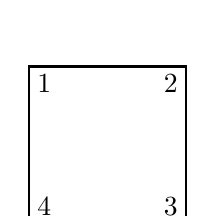
\begin{tikzpicture}
		\node[draw=black, thick,minimum width=2cm,minimum height=2cm] (rect) at (0,0) {};
		\foreach \anc/\n in {south west/4,north west/1,north east/2,south east/3}{
			\node[anchor=\anc] at (rect.\anc) {\n};
		}
	\end{tikzpicture}
	\end{equation*}
	Now, there are four rotations of this square about its center, resulting in the permutations (falling to the shorter notation) $(1\;2\;3\;4), (2\;3\;4\;1), (3\;4\;1\;2), (4\;1\;2\;3)$. There are two reflections about a line passing through the center and one of the vertices (as if the line passes through one vertex, it also passes by the one directly across the center), those result in the permutations $(1\;4\;3\;2)$ and $(3\;2\;1\;4)$. There are also the two reflections about a line passing through the center and a middle of one of the sides, there we get $(2\;1\;4\;3)$ and $(4\;3\;2\;1)$. But that is all the $8$ symmetries of this square, thus we have a homomorphism $D_8 \to S_4$.
\end{proof}

% Problem 2.5
\begin{problem}
\end{problem}

\begin{solution}
	Let $D_{2n}$ be a dihedral group, i.e. the group of symmetries of a regular polygon with $n$ vertices. Let $x$ be a reflection about the center of the polygon and any vertex. Clearly, it must hold that $x^2 = e$, as reflecting about the same line twice returns all the vertices to their original places. Let $y$ be a counterclockwise rotation by $2\pi/n$. Rotating the polygon $n$ times gives us back the original polygon, and thus $y^n=e$.  Now, notice that composing those two symmetries like $xyxy$ gives us back the original polygon, thus $(xy)^2=e$. Manipulating this equation we get $yx=xy^{-1}=xy^{n-1}$ (as $y^{-1}=y^{n-1}$). 
	
	Using these relation we can simplify any product in $D_{2n}$. Suppose $x^{i_1}y^{j_1}x^{i_2}y^{j_2}\dots$ is such a product and without loss of generality suppose $i_k < 2$ and $j_k < n$ for $k \in \mathbb{N}$ (due to the $x^2=e$ and $y^n=e$ relations). Now, we can use the relation $yx = xy^{n-1}$ to move all the $x$ in the product to the right. Thus we can in fact simplify any product in $D_{2n}$ to $x^i y^j$ for $0 \leq i < 2, 0 \leq j < n$.
\end{solution}

% Problem 2.6
\begin{problem}
\end{problem}

\begin{solution}
	For the case $n=1$, we can easily take $g=h$, since $\abs{g}=2$, we have $gg=e$ and thus $\abs{gh}=1$ as needed.
	
	Now suppose $n > 1$. Now consider the group $D_{2n}$. By Problem II.2.5. there are elements $x,y \in D_{2n}$ such that $\abs{x}=2$, $\abs{y}=n$ and $\abs{xy}=2$. Let us define $g = xy$ and $h = x$ (so that $\abs(g)=\abs(h)=2$). We have $gh = xyx = y^{-1}$ and thus $\abs{gh}=\abs{y^{-1}}=\abs{y}=n$.
\end{solution}

% Problem 2.7
\begin{problem}
\end{problem}

\begin{solution}
	By Problem II.2.6. any element of $D_{2n}$ can be written as a product $xy^i$ or $y^i$, $0 \leq i < n$. Now, consider the elements of the form $y^i$, $0 < i < n$. For $y^i$ to commute with $x$, we need to have $x y^i=y^i x$ by definition. But $x y^i = x y y^{i-1} = y^{-i} x$ (as $\abs{xy}=2$). But that means $y^i = y^{-i}=(y^i)^{-1}$ and thus $\abs{y^i}=2$. But by Proposition I.1.13. we know that $\abs{y^i}=\frac{\abs{y}}{\gcd(i, \abs{y}}=\frac{n}{\gcd(i,n)}=2$. So in particular $\gcd(i,n)=\frac{n}{2}$. Since $i < n$, it follows that $i=\frac{n}{2}$.
		
	Now consider elements of the form $xy^i$. If such an element commutes with everything, it has to commute with $x$ in particular. We have $xxy^i=y^i$ and $xy^ix=x^2y^{-i}=y^{-i}$. Now this can only happen for $i = \frac{n}{2}$. Now, it must also commute with $y$. We have $yxy^i=xy^{i-1}$ and $xy^{i}y=xy^{i+1}$. Now, $xy^{i-1}=xy^{i+1}$ would mean $y^{i-1}=y^{i+1}$, which in turn would mean $y^2=e$. But that only happens if $n=2$.
	
	Therefore we have found that there are no elements that commute with everything for groups $D_{2n}$ where $n$ is odd. In the case $n=2$, $y$ and $xy$ commute with everything. In the case $n > 2$, the only such element is $y^{\frac{n}{2}}$, which of course only exists if $n$ is even.
\end{solution}

% Problem 2.8
\begin{problem}
\end{problem}

\begin{solution}
	[not interested]
\end{solution}

% Problem 2.9
\begin{problem}
\end{problem}

\begin{solution}
	Let $n\in\mathbb{N}$ and $\equiv$ be the 'congruence modulo $n$' relation. Now, let $a,b,c \in \mathbb{Z}$ be numbers. We will prove that $\equiv$ is an equivalence relation:
	\begin{itemize}
		\item We have $a-a=0$ and trivially $n | 0$, thus $a \equiv a$.
		\item Suppose $a \equiv b$. Then $n | (b - a)$ by definition. But then there is $k \in \mathbb{Z}$ such that $(b - a) = kn$. But then $-(b - a) = (a - b) = -kn$, and that means $n | (a - b)$. Therefore $b \equiv a$.
		\item Suppose $a \equiv b$ and $b \equiv c$. Then we have $n | (b - a)$ and $n | (c - b)$. But then there are $k,l \in \mathbb{Z}$ such that $(b - a) = kn$ and $(c - b) = ln$. Summing those two equations we obtain $(b - a) + (c - b) = (c - a) = kn + ln = (k + l)n$ and thus $a \equiv c$.
	\end{itemize}
\end{solution}

% Problem 2.10
\begin{problem}
\end{problem}

\begin{solution}
	Let $\mathbb{Z}/n\mathbb{Z}$ be a cyclic group. The group is the set of equivalence classes of congruence modulo $n$ on $\mathbb{Z}$. Clearly, the $n$ elements $[0]_n,[1]_n,\dots,[n-1]_n$ are all distinct, as if we had $[i]_n = [j]_n$, $0 \leq i < j < n$ (clearly it does not matter if $i < j$ or $j < i$), then $i \equiv j$ so $n | (j - i)$ and thus $j - i = kn$ for some $k \in \mathbb{Z}$. But that is a contradiction, as $i < j < n$ so $j - i < n$ and $i \neq j$ so $j - i \neq 0$.
	
	Now, let $m \in \mathbb{Z}$ be a number such that $m < 0$ or $n \leq m$. Then we can divide $m$ by $n$ such that we get $n = km + i$ for some $k \in \mathbb{Z}$ and $0 \leq i < n$. But that means $n | (m - i)$ and thus $m \equiv i$ and therefore $[m]_n = [i]_n$.
	
	Thus, there are precisely $n$ elements of $\mathbb{Z}/n\mathbb{Z}$ given above.
\end{solution}

% Problem 2.11
\begin{problem}
\end{problem}

\begin{solution}
	Let $n \in \mathbb{Z}$ be an odd integer. Then we can write $n=2k+1$ for some $k \in \mathbb{Z}$ by the definition of an odd integer. Then we have $n^2=(2k+1)^2=4k^2+4k+1$. Now, there are two possibilities, either $k$ is even, or $k$ is odd.
	
	Suppose $k$ is even, then $k = 2l$ for some $l \in \mathbb{Z}$. But then $n^2=16l^2+8l+1$, which means $8 | n^2-1$, so that $n \equiv 1 \mod 8$.
	
	Now suppose $k$ is odd, then $k=2l+1$ for some $l \in \mathbb{Z}$. Then $n^2=16l^2+16l+4+8l+4+1=16l^2+24l+9$ so that again $8 | n^2 - 1$ and thus $n \equiv 1 \mod 8$.
\end{solution}

% Problem 2.12
\begin{problem}
\end{problem}

\begin{solution}
	If there are some nonzero integers $a, b, c \in \mathbb{Z}$ such that $a^2+b^2=3c^2$, then the equation $[a]^2_4+[b]^2_4=3[c]^2_4$ in $\mathbb{Z}/4\mathbb{Z}$ would also have to hold. Now, notice that for any $n \in \mathbb{Z}$, $[n]^2_4$ can either equal $0$ (if $n$ is even) or $1$ ($n$ odd). Therefore for the equation to hold in $\mathbb{Z}/4\mathbb{Z}$, $a, b, c$ all have to be even. Let $a=2k, b=2l, c=2m$ for some $k,l,m \in \mathbb{Z}$. Then we have $k^2+l^2=3m^2$. But again, $k,l,m$ have to be even. We can continue this process until we reach $1$ for some of the factors, proving that indeed $a^2+b^2=3c^2$ does not have a non trivial solution in $\mathbb{Z}$.
\end{solution}

% Problem 2.13
\begin{problem}
\end{problem}

\begin{solution}
	Suppose that $m,n \in \mathbb{Z}$ are numbers such that $\gcd(m,n) = 1$. Then by Corollary II.2.5. we see that $[m]_n$ is a generator of $\mathbb{Z}/n\mathbb{Z}$. But there is some $a \in \mathbb{Z}$ such that $a[m]_n=[am]_n=[1]_n$. But that means $am \equiv 1 \mod n$, so $n | (am - 1)$, and therefore $(am - 1) = cn$. But that shows exactly what we required, there are $a,b \in \mathbb{Z}$ such that $am - cn = am + bn = 1$.
	
	Conversely, suppose there are integers $a, b$ such that $am+bn=1$. But then $[am+bn]_n=[am]_n=[1]_n$. But then if $[x]_n \in \mathbb{Z}/n\mathbb{Z}$ is any element of the group, we have $[x]_n=x[1]_n=x[am]_n=xa[m]_n$. But that means $[m]_n$ generates the group, and thus by Corollary II.2.5. $\gcd(m,n)=1$ must hold.
\end{solution}

% Problem 2.14
\begin{problem}
\end{problem}

\begin{solution}
	Suppose $a \equiv a' \mod n$ and $b \equiv b' \mod n$. Then we have $n | (a' - a)$ and thus $a' - a = kn$, similarly we have $b' - b = ln$, for some $k,l \in \mathbb{Z}$. Now, $a'b'-ab=a'b'-(a'-kn)(b'-ln)=a'b'-(a'b'-a'ln-b'kn+lkn^2)=(-a'l-b'k+lkn)n$. But then $n | (a'b'-ab)$, so $[ab]_n=[a'b']_n$. But that means that multiplication of equivalence classes is well-defined.
\end{solution}

% Problem 2.15
\begin{problem}
\end{problem}

\begin{solution}
	Let $n > 0$ be an odd integer.
	\begin{itemize}
		\item Let $m$ be an integer and $\gcd(m,n)=1$. By Exercise II.2.13. there are integers $a,b$ such that $am+bn=1$. We then have $4am+4bn=4am+2n+4bn-2n=2a(2m+n)+(2b-a)2n=4$. That means $\gcd(2m+n,2n) | 4$, as the $\gcd$ must divide the whole equation. But $2m+n$ is odd, since $n$ is odd. Thus $\gcd(2m+n,2n)=1$.
		\item Now, let $r$ be an integer and suppose $\gcd(r,2n)=1$. Then we have, again by Exercise II.2.13., $ar+b2n=1$ for some integers $a,b$. But then we have $ar-an+b2n+an=a(r-n)+(2b+a)n=2a\frac{r-n}{2}=(2b-a)n=1$. Using the result of Exercise II.2.13. again we get $\gcd(\frac{r-n}{2},n)=1$.
		\item Consider the function $f: (\mathbb{Z}/n\mathbb{Z})^* \to (\mathbb{Z}/2n\mathbb{Z})^*$ defined as $f([m]_n)=[2m+n]_{2n}$. Now, this function is well defined, as if $[m]_n \in (\mathbb{Z}/n\mathbb{Z})^*$ we have $\gcd(m,n)=1$ so $\gcd(2m+n,2n)=1$ and thus $[2m+n]_{2n} \in (\mathbb{Z}/2n\mathbb{Z})^*$. Now, define a function $g: (\mathbb{Z}/2n\mathbb{Z})^* \to (\mathbb{Z}/n\mathbb{Z})^*$ as $g([r]_{2n})=[\frac{r-n}{2}]_n$. This function is again well defined. Now, $gf([m]_n)=g([2m+n]_{2n})=[\frac{2m}{2}]_n=[m]_n$ and thus $g$ is a left-inverse of $f$. $fg([r]_{2n})=f([\frac{r-n}{2}]_n)=[2\frac{r-n}{2} + n]_{2n}=[r-n+n]_{2n}=[r]_{2n}$ and thus $g$ is also a right-inverse of $f$. Therefore $f$ is a bijective function. But that means $(\mathbb{Z}/n\mathbb{Z})^*$ and $(\mathbb{Z}/2n\mathbb{Z})^*$ are isomorphic. \qedhere
	\end{itemize}
\end{solution}

% Problem 2.16
\begin{problem}
\end{problem}

\begin{solution}
	To find the last digit of $1238237^{18238456}$ we will work in $\mathbb{Z}/10\mathbb{Z}$. We have $[1238237]_{10}=[7]_{10}$. Now $[7^2]_{10}=[9]_{10}$, $[7^3]_{10}=[3]_{10}$, $[7^4]_{10}=[1]_{10}$. But $[18238456]_{4}=0$, and thus the last digit is $1$.	
\end{solution}

% Problem 2.17
\begin{problem}
\end{problem}

\begin{solution}
	Suppose $m \equiv m' \mod n$. Then $n | (m' - m)$ so $m' - m = kn$ for some integer $k$. Now, suppose that $\gcd(m,n)=1$. Then by Exercise II.2.13. there are integers $a,b$ such that $am+bn=1$. But $m = m' - kn$, so we have $a(m' - kn)+bn=am'-akn+bn=am'+(b-ak)n=1$, and thus $\gcd(m',n)=1$. 
	
	If $\gcd(m',n)=1$, then again there are integers $a,b$ such that $am'+bn=1$. But $m' = kn - m$, so $am'+bn=a(kn - m) + bn=akn-am+bn=(-a)m+(ak+b)n=1$ and thus $\gcd(m,n)=1$.
\end{solution}

% Problem 2.18
\begin{problem}
\end{problem}

\begin{solution}
	Define the function as follows. For $[m]_d$ we move every element up to $d$ $m$ places to the right, wrapping around. This way, $[0]_d$ is the identity permutation, $[1]_d$ is the permutation $(d\;1\;2\;\dots\;d-2\;d-1\;d+1\;\dots n)$. Composing this morphism gets us the permutation $(d-1\;d\;1\dots)$ etc. So indeed, those morphisms preserve the structure.
\end{solution}

% Problem 2.19
\begin{problem}
\end{problem}

\begin{solution}
	Multiplication table for $(\Z{5})^*$:
	
	\begin{center}
		\renewcommand{\arraystretch}{1.3}
		\begin{tabular}{c||c|c|c|c}
			$\cdot$ & $[1]$ & $[2]$ & $[3]$ & $[4]$ \\
			\hline\hline
			$[1]$ & $[1]$ & $[2]$ & $[3]$ & $[4]$ \\ 
			\hline
			$[2]$ & $[2]$ & $[4]$ & $[1]$ & $[3]$ \\ 
			\hline
			$[3]$ & $[3]$ & $[1]$ & $[4]$ & $[2]$ \\ 
			\hline
			$[4]$ & $[4]$ & $[3]$ & $[2]$ & $[1]$ \\ 
		\end{tabular}
	\end{center}

	Multiplication table for $(\Z{12})^*$:
	
	\begin{center}
		\renewcommand{\arraystretch}{1.3}
		\begin{tabular}{c||c|c|c|c}
			$\cdot$ & $[1]$ & $[5]$ & $[7]$ & $[11]$ \\
			\hline\hline
			$[1]$ & $[1]$ & $[5]$ & $[7]$ & $[11]$ \\ 
			\hline
			$[5]$ & $[5]$ & $[1]$ & $[11]$ & $[7]$ \\ 
			\hline
			$[7]$ & $[7]$ & $[11]$ & $[1]$ & $[5]$ \\ 
			\hline
			$[11]$ & $[11]$ & $[7]$ & $[5]$ & $[1]$ \\ 
		\end{tabular}
	\end{center}

	Now note that we can clearly see $(\Z{12})^*$ has $3$ elements of order $2$, but $(\Z{5})^*$ has two elements of order $4$ and a single element of order $2$. Therefore we cannot relabel the elements in a way the two groups would correspond.
\end{solution}

\subsection{The category $\mathsf{Grp}$}

% Problem 3.1
\begin{problem}
\end{problem}

\begin{solution}
	Let $\C$ be a category with products and $\varphi: G \to H$ a morphism in $\C$. Now, if we have products $G \times G$ and $H \times H$ with the morphisms $\pi_G,\pi'_G: G \times G \to G$ and $\pi_H,\pi'_H: H \times H \to H$, we can use the universal property of products as follows: Since $H \times H$ with $\pi_H,\pi'_H$ satisfies the universal property, for any object $X$, such that there are morphisms $f_H,f'_H: X \to H$, there is a unique morphism $X \to H \times H$. Now notice that for $G \times G$ we have two morphisms $\varphi \circ \pi_G: G \times G \to H$ and $\varphi \circ \pi'_G: G \times G \to H$. Therefore due to the unique property of products there is a unique morphism $\varphi \times \varphi: G \times G \to H \times H$ such that $\pi_H \circ (\varphi \times \varphi) = \varphi \circ \pi_G$ and $\pi'_H \circ (\varphi \times \varphi) = \varphi \circ \pi'_G$.
\end{solution}

% Problem 3.2
\begin{problem}
\end{problem}

\begin{solution}
	Let $\C$ be a category with products and $\varphi: G \to H$ and $\psi: H \to K$ morphisms in $\C$. By Exercise II.3.1. there are then morphisms $(\varphi \times \varphi): G \times G \to H \times H$ and $(\psi \times \psi): H \times H \to K \times K$ and also $(\psi \circ \varphi) \times (\psi \circ \varphi): G \times G \to K \times K$ (since $\psi \circ \varphi: G \to K$) compatible with the natural projections. Now we will prove the diagram
	
	\begin{equation*}
		\begin{tikzcd}[column sep=huge]
			& & K \\
			G \times G
			\arrow[r, "(\psi \times \psi) \circ (\varphi \times \varphi)"]
			\arrow[urr, bend left=20, "\psi \circ \varphi \circ \pi_G"]
			\arrow[drr, bend right=20, "\psi \circ \varphi \circ \pi'_G"'] &
			K \times K
			\arrow[ur, "\pi_K"]
			\arrow[dr, "\pi'_K"'] & \\
			& & K \\
		\end{tikzcd}
	\end{equation*}
	
	commutes. Note that by Exercise II.3.1. we have $\pi_K \circ (\psi \times \psi) = \psi \circ \pi_H$ and $\pi_H \circ (\varphi \times \varphi) = \varphi \circ \pi_G$. Thus we have
	
	\begin{equation*}
		\begin{aligned}
			\pi_K \circ (\psi \times \psi) \circ (\varphi \times \varphi) &={} \psi \circ \pi_H \circ (\varphi \times \varphi)\\ &={} \psi \circ \varphi \circ \pi_G
		\end{aligned}
	\end{equation*}
	
	 and similarly for the other side. But we know $(\psi \circ \varphi) \times (\psi \circ \varphi)$ is the unique morphism making the diagram commute (by Exercise II.3.1.) and therefore $(\psi \circ \varphi) \times (\psi \circ \varphi) = (\psi \times \psi) \circ (\varphi \times \varphi)$.
\end{solution}

% Problem 3.3
\begin{problem}
\end{problem}

\begin{solution}
		Suppose $G$ and $H$ are abelian groups. Consider the product of those groups, $G \times H$, with the two natural homomorphisms $i_G: G \to G \times H$ ($g \mapsto (g, e_H)$) and $i_H: H \to G \times H$ ($h \mapsto (e_G, h)$). For this construction to satisfy the universal property of coproducts in $\mathsf{Ab}$, for any abelian group $Z$ such that there are homomorphisms $f_G: G \to Z$ and $f_H: H \to Z$, there must be a unique homomorphism $\sigma: G \times H \to Z$ making
		\begin{equation*}
			\begin{tikzcd}
				G
					\arrow[drr, bend left=20, "f_G"]
					\arrow[dr, "i_G" swap]
					& &\\
				&
					G \times H
						\arrow[r, "\sigma"]
					& Z\\
				H
					\arrow[urr, bend right=20, "f_H"']
					\arrow[ur, "i_H"]
					& &
			\end{tikzcd}
		\end{equation*}
		commute. Now, the only choice for $\sigma$ is given by the set-function $\sigma((a,b))=f_G(a)f_H(b)$. We have to check that $\sigma$ is a group homomorphism.
		We have
		\begin{equation*}
			\begin{aligned}
				\sigma((a,b)(c,d)) &= \sigma((ac,bd))\\
				&= f_G(ac)f_H(bd)\\
				&= f_G(a)f_G(c)f_H(b)f_H(d)\\
				&= f_G(a)f_H(b)f_G(c)f_H(d)\\
				&=\sigma((a,b))\sigma((c,d))
			\end{aligned}
		\end{equation*} 
		precisely because $Z$ is commutative. Therefore, $G \times H$ satisfies the universal propery of coproducts in $\C$.
\end{solution}

% Problem 3.4
\begin{problem}
\end{problem}

\begin{solution}
	$H$ does not necessarily have to be the trivial group. We can consider a countably infinite product $G = H \times H \dots$. Then indeed $G \cong G \times H$.
\end{solution}

% Problem 3.5
\begin{problem}
\end{problem}

\begin{solution}
	Let $\mathbb{Q}=G \times H$. If both $G, H$ are trivial, then $\mathbb{Q}$ would be trivial, and thus, without loss of generality, say that $G$ is non-trivial. Now, consider the canonical projection $\pi_G$.
	
	We will show that $\pi_G$ is in fact an injective homomorphism. First of all, notice that for $m \neq 0$ and any $g \in G$ such that $g^m = e_G$ we have $(g, e_H)^m = (g^m, e_H) = (e_G, e_H)$. But $\mathbb{Q}$ has no non-zero elements of finite order, and thus $g = e_G$.
	
	Now suppose that $\pi_G$ is not an injective homomorphism and thus there are two rational numbers $\frac{a_1}{b_1}, \frac{a_2}{b_2}$, such that $a_1, a_2, b_1, b_2 \neq 0 \in \mathbb{Z}$ and $\frac{a_1}{b_1} \neq \frac{a_2}{b_2}$, for which $\pi_G(\frac{a_1}{b_1}) = \pi_G(\frac{a_2}{b_2})$. Then we have $\pi_G(\frac{a_1}{b_1})^{b_1 b_2} = \pi_G(a_1)^{b_2} = \pi_G(1)^{a_1 b_2}$ and similarly $\pi_G(\frac{a_2}{b_2}) = \pi_G(1)^{a_2 b_1}$ (because $\pi_G$ is a group homomorphism). Then we must have $\pi_G(1)^{a_1 b_2} = \pi_G(1)^{a_2 b_1}$ and thus $\pi_G(1)^{a_1 b_2 - a_2 b_1} = e_G$. But that means $\pi_G(1) = e_G$ (by the last paragraph) and thus $\pi_G$ maps every integer to $e_G$.
	
	Now suppose $\frac{a}{b}$ is a rational number, $a, b \neq 0 \in \mathbb{Z}$. Now $\pi_G(\frac{a}{b})^b = \pi_G(a) = e_G$. But by the same argument of order we thus have $\pi_G(\frac{a}{b}) = e_G$. That means $\pi_G$ maps everything to $e_G$. Since $\pi_G$ is necessarily a surjective homomorphism, $G$ is trivial, a contradiction. Therefore $\pi_G$ must be an injective homomorphism. But since $\pi_G((e_G,h))=e_G$ for all $h \in H$ by definition, $H$ must necessarily be trivial.
\end{solution}

% Problem 3.6
\begin{problem}
\end{problem}

\begin{solution}
	Going point by point:
	\begin{itemize}
		\item Let $f: C_2 \to S_3$ be defined as $f(e) = (1\;2\;3)$ and $f(x) = (2\;1\;3)$. Then $f(x^n)=e$ if $2 | n$ or $f(x^n)=(2\;1\;3)$ otherwise. Thus this is an injective homomorphism. Now, let $g: C_3 \to S_3$ be defined as $g(e)=(1\;2\;3)$, $g(x)=(2\;3\;1)$ and $g(x^2)=(3\;1\;2)$. Now, $g(x)g(x)=(3\;1\;2)=g(x^2)$, and $g(x)g(x^2)=(1\;2\;3)$, so it is indeed an injective homomorphism.
		\item Suppose $C_2 \times C_3$ is the coproduct of $C_2$ and $C_3$ in $\mathsf{Grp}$. By the universal property of coproducts,  as there are morphisms $C_2 \to S_3$ and $C_3 \to S_3$, this means there is a unique homomorphism $\sigma: C_2 \times C_3 \to S_3$, such that $\sigma i_{C_2} = f$ and $\sigma i_{C_3} = g$.
		\item Now, notice that $i_{C_2}$ must necessarily map an element $x \in C_2$ to $(x, e_{C_3})$, and similarly for $i_{C_3}$. But then we have $f(x_1)g(x_2)=\sigma((x_1, e_{C_3})(e_{C_2}, x_2))=\sigma((x_1, x_2))=\sigma((e_{C_2}, x_2)(x_1, e_{C_3})=g(x_2)f(x_1)$. But we have, for example, $(2\;1\;3)(2\;3\;1)=(3\;2\;1)$ and $(2\;3\;1)(2\;1\;3)=(1\;3\;2)$. Thus $\sigma$ cannot exist (precisely because $S_3$ is not commutative). \qedhere
	\end{itemize}
\end{solution}

% Problem 3.7
\begin{problem}
\end{problem}

\begin{solution}
	Let $\mathbb{Z} \ast \mathbb{Z}$, $C_2 \ast C_3$ be a coproduct in $\Cgrp$. Let $A$ be a group and $\alpha': C_2 \ast C_3 \to $ and $\alpha'': C_2 \ast C_3 \to A$ any two homomorphisms. Consider the diagram
	
	\begin{equation*}
		\begin{tikzcd}
			\mathbb{Z} 
			\arrow[rr]
			\arrow[dr, "i_\mathbb{Z}"] & & 
			C_2
			\arrow[dr, "i_{C_2}"]
			\arrow[drr, bend left=20, "\alpha' i_{C_2}"] & & \\
			& \mathbb{Z} \ast \mathbb{Z}
			\arrow[rr, dashrightarrow, "\sigma"] & & 
			C_2 \ast C_3 
			\arrow[r, shift left, "\alpha'"]
			\arrow[r, shift right, "\alpha''"'] & A \\
			\mathbb{Z}
			\arrow[rr]
			\arrow[ur, "i'_\mathbb{Z}"'] & & 
			C_3
			\arrow[ur, "i_{C_3}"']
			\arrow[urr, bend right=20, "\alpha'' i_{C_3}"'] & & \\
		\end{tikzcd}
	\end{equation*}
	
	Now, by the universal property of coproducts, $\sigma$ is a unique homomorphism making the diagram commute. Notice, that by the universal property of coproducts we can also see $\alpha'$ is the unique homomorphism making the right half of the diagram commute. But that means $\alpha' = \alpha''$ and thus $\sigma$ is an epimorphism. But that means it is a surjective set-function and thus a surjective homomorphism.
\end{solution}

% Problem 3.8
\begin{problem}
\end{problem}

\begin{solution}
	Define a group $G$ as the group generated by two elements $x, y$ such that $x^2=e_G$ and $y^3=e_G$. Then we can define group homomorphisms $i_{C_2}: C_2 \to G$ and $i_{C_3}: C_3 \to G$ as follows: $i_{C_2}(e_{C_2})=e_G$, $i_{C_2}(c_2)=x$, $i_{C_3}(e_{C_3})=e_G$, $i_{C_3}(c_3)=y$, $i_{C_3}(c_3^2)=y^2$.
	
	Suppose $Z$ is any group, and $f: C_2 \to Z$ and $g: C_3 \to Z$ group homomorphisms. To prove that $G$ satisfies the universal property of coproducts in $\mathsf{Grp}$ we have to construct a group homomorphism $\sigma: G \to Z$, such that $\sigma i_{C_2} = f$ and $\sigma i_{C_3} = g$. Now notice that we must have $\sigma i_{C_2} (c_2) = \sigma(x) = f(c_2)$ and $\sigma i_{C_3} = \sigma(y) = g(c_3)$. Since $x$ and $y$ generate every element of $G$, this is enough for us to construct $\sigma$. If $x^{i_0} y^{j_0} x^{i_1} y^{j_1} \dots$ where $0 \leq i_0, i_1, \dots < 2$ and $0 \leq j_0, j_1 \dots < 3$ is an element of $G$, we define $\sigma(x^{i_0} y^{j_0} x^{i_1} y^{j_1} \dots)  = f(c_2)^{i_0} g(c_3)^{j_0} \dots$.
	
	It is clear that $\sigma$ is a homomorphism that makes the relevant diagram commute.
\end{solution}

% Problem 3.9
\begin{problem}
\end{problem}

\begin{solution}
	The definition of the fiber product is pretty straightforward, and follows straight from the definition for $\mathsf{Set}$. We only have to check that the definition indeed results in a group and satisfies the required universal property. Let $A,B,C$ be groups and $\alpha: A \to C$, $\beta: B \to C$ group homomorphisms. Define $A \times_C B = \set{(a,b) \in A \times B \mid \alpha(a)=\beta(b)}$.
	
	To check that this construction is a group, we will take the operation to be the same as the one on $A \times B$, i.e. $(a,b)(c,d)=(ac,bd)$. This operation is well-defined, as we have $\alpha(a)=\beta(b)$ and $\alpha(c)=\beta(d)$, and since $\alpha, \beta$ are group homomorphisms, $\alpha{ab}=\alpha(a)\alpha{b}=\beta{c}\beta{d}=\beta{cd}$. Now, we have to prove that $(e_A, e_B)$ is an element of the group. But we have $\alpha(e_A)=e_C=\beta(e_B)$, again because they are homomorphisms. Now, suppose $(a,b) \in A \times_C B$. Then $\alpha(a)=\beta(b)$, so $(\alpha(a))^{-1}=(\beta(b))^{-1})$ and again because they are homomorphisms, $\alpha(a^{-1})=\beta(b^{-1})$. Therefore $(a^{-1}, b^{-1}) \in A \times_C B$, but that is an inverse of $(a, b)$. Thus $A \times_C B$ is a group.
	
	Now, we have to prove that this construction satisfies the universal property of a fiber product. Suppose $Z$ is a group and $f, g$ the respective homomorphisms, such that $\alpha f = \beta g$. To ensure the commutativity of the respective diagram, we have to define $\sigma: Z \to A \times_C B$ as follows: $\sigma(z)=(f(z),g(z))$.  It is well defined, as we have $(\alpha f)(z) = (\beta g)(z)$, so $\alpha (f(z))=\beta(g(z))$. To see that this is a group homomorphism, note that $\sigma(z_1 z_2) = (f(z_1z_2), g(z_1z_2)) = (f(z_1)f(z_2),g(z_1)g(z_2))=(f(z_1), g(z_1))(f(z_2), g(z_2))=\sigma(z_1)\sigma(z_2)$.

	The commutativity of the diagram follows from the definition easily, note that we have $(\pi_A \sigma)(z)=\pi_A(\sigma(z))=\pi_A((f(z), g(z)))=f(z)$ so $\alpha \pi_A \sigma = \alpha f$ and similarly for the other side of the diagram.
	
	To define the fibered coproduct in $\mathsf{Ab}$ we require knowledge of quotients, which have yet to be introduced.
\end{solution}

\subsection{Group homomorphisms}

% Problem 4.1
\begin{problem}
\end{problem}

\begin{solution}
	Suppose $m | n$ and $a \equiv a' \mod n$. Then $n | (a' - a)$. But then $m | (a' - a)$, and thus $[a]_m = [a']_m$.
	
	To check it makes the diagram commute, notice that for any $z \in \mathbb{Z}$ we have $(\pi^n_m \pi_n)(z)=\pi^n_m([z]_n)=[z]_m=\pi_m(z)$ by the definition of the function.
	
	To verify it is indeed a group homomorphism, let $a,b$ be elements of $\mathbb{Z}_n$. Then we have $\pi^n_m(a+b)=[a+b]_m=[a]_m + [b]_m = \pi^n_m(a) + \pi^n_m(b)$.
	
	Thus $\pi^n_m$ is a well-defined group homomorphism that makes the diagram commute. The hypothesis $m | n$ is necessary as the order of all elements of $\mathbb{Z}_n$ divides $n$ and the order of all elements of $\mathbb{Z}_m$ divides $m$, and it also must hold that $\abs{\pi^n_m(z)} \mid \abs{z} \mid n$. Now if $m \nmid n$, then $\pi^n_m([1]_n)=[1]_m$ but $\abs{\pi^n_m([1]_n)}=m \nmid n$, a contradiction.
\end{solution}

% Problem 4.2
\begin{problem}
\end{problem}

\begin{solution}
	The homomorphism is defined pretty explicitly so we can easily check that the image of the homomorphism is the set $\set{(0,0),(1,1)}$, which is in fact not isomorphic to the set underlying $C_2 \times C_2$. We can actually show that there is no such isomorphism. 
	
	In fact, there is no isomorphism of the two groups. The generator of $C_4$ has order $4$, but there is no such element in $C_2 \times C_2$ (all non-zero elements have order $2$).
\end{solution}

% Problem 4.3
\begin{problem}
\end{problem}

\begin{solution}
	Suppose $G$ is a group of order $n$ isomorphic to $\mathbb{Z}/n\mathbb{Z}$. Let $\varphi: \Z{n} \to G$ be a group isomorphism. There is an element of order $n$ in $\Z{n}$, namely $[1]_n$. By Proposition II.4.8. $\abs{\varphi([1]_n)}=\abs{[1]_n}=n$, thus $G$ contains an element of order $n$.
	
	Suppose the converse holds, i.e. $G$ is a group of order $n$ which contains an element $x$ of 
	order $n$. Because $x$ has order $n$, the elements $x^0, x^1, \dots, x^{n-1}$ must make up all of G (if some of those elements were equal, it would be a contradiction to the order of $x$ by cancellation). We can define a homomorphism $\varphi: \Z{n} \to G$ as $\varphi([i]_n) = x^i$.
	
	This is a homomorphism as $\varphi([i]_n + [j]_n) = \varphi([i + j]_n) = x^{i + j} = x^i x^j = \varphi([i]_n) \varphi([j]_n)$.
	
	Now define $\rho: G \to \Z{n}$ as $\rho(x^i) = [i]_n$. It is easy to see that this is an inverse of $\varphi$ and thus $\varphi$ is an isomorphism of groups.
\end{solution}

% Problem 4.4
\begin{problem}
\end{problem}

\begin{solution}
	\begin{itemize}
		We will consider the groups one by one:
		
		\item Consider $(\mathbb{Z}, +)$. Notice that any element $z \in \mathbb{Z}$ is equal to $z \cdot 1$. Therefore any homomorphism $\varphi: (\mathbb{Z}, +) \to G$ (where $G$ is any group) is uniquely determined by $\varphi(1)$. Let $G = \mathbb{Q}$ (or $\mathbb{R}$) and suppose $\varphi(1) = \frac{a}{b}$ for some $a, b \neq 0 \in \mathbb{Z}$. Then $\varphi(z) = z \varphi(1) = z \frac{a}{b} = \frac{z \cdot a}{b}$. But that clearly means there is no number $z$ such that $\varphi(z) = \frac{a}{b+1}$. Thus $\varphi$ is not surjective and therefore it cannot be an isomorphism.
		
		\item Now consider $(\mathbb{Q}, +)$. Let $x, y \in \mathbb{Q}$, clearly, we can always find non-zero integers $a, b$ such that $a x = b y$. However, this is not true in $\mathbb{R}$, if for example $x = \sqrt{2}$ and $y = 1$. Thus the two groups cannot be isomorphic.
		
		\item $(\mathbb{R}, +)$ and $(\mathbb{C}, +)$ are in fact isomorphic. However the construction of the isomorphism is fairly involved. \qedhere
	\end{itemize}
\end{solution}

% Problem 4.5
\begin{problem}
\end{problem}

\begin{solution}
	Notice that $i$ has order $4$ in $(\mathbb{C} \setminus 0, \cdot)$. However, there is no element of $(\mathbb{R} \setminus 0, \cdot)$ of order $4$. Since isomorphism preserves order of elements, it follows that the two groups are not isomorphic.
\end{solution}

% Problem 4.6
\begin{problem}
\end{problem}

\begin{solution}
	The two groups are not isomorphic. Suppose there is an isomorphism $\varphi: (\mathbb{Q}, +) \to (\mathbb{Q}^{>0}, \cdot)$. Let $y$ be a number such that $\varphi(y) = 2$ (there must be such a number because $\varphi$ is an isomorphism). Now we can find a number $x \in \mathbb{Q}$ such that $x + x = y$ in $(\mathbb{Q}, +)$. But then $\varphi(y) = \varphi(x + x) = \varphi(x) \varphi(x) = \varphi^2(x) = 2$. But we know there is no number in $\mathbb{Q}$ with this property.
\end{solution}

% Problem 4.7
\begin{problem}
\end{problem}

\begin{solution}
	Let $G$ be a group and $g, h$ be elements $G$. 
	
	Consider the function $\varphi: G \to G$, $\varphi(g) = g^{-1}$. Suppose $\varphi$ is a group homomorphism. Then we have $hg = (g^{-1} h^{-1})^{-1} = \varphi(g^{-1} h^{-1}) = \varphi(g^{-1})\varphi(h^{-1}) = gh$. But that means precisely that $G$ is an abelian group. Now suppose $G$ is abelian. Then $\varphi(gh) = (gh)^{-1} = h^{-1} g^{-1} = \varphi(h) \varphi(g) = \varphi(g) \varphi(h)$. And thus $\varphi$ is a group homomorphism.
	
	Consider the function $\psi: G \to G$, $\psi(g) = g^2$. Suppose $\psi$ is a group homomorphism. Then $ghgh = (gh)^2 = \psi(gh) = \psi(g) \psi(h) = g^2 h^2 = gghh$. By cancellation we then have $hg = gh$ and thus $G$ is abelian. Now suppose $G$ is abelian. Then $\psi(gh) = (gh)^2 = ghgh = gghh = g^2 h^2 = \psi(g) \psi(h)$. And thus $\psi$ is a group homomorphism.
\end{solution}

% Problem 4.8
\begin{problem}
\end{problem}

\begin{solution}
	Let $G$ be a group, and let $g \in G$. Consider the function $\gamma_g: G \to G$, $\gamma_g(a) = gag^{-1}$. Let $a, b \in G$. Then $\gamma_g(ab) = g(ab)g^{-1} = gag^{-1}gbg^{-1} = \gamma_g(a) \gamma_g(b)$. Thus $\gamma_g$ is a group homomorphism. Now let $\varphi_g: G \to G$ be a function defined as $\varphi_g(a) = g^{-1}ag$. Clearly this is also a group homomorphism. For $a \in G$ we have $(\gamma_g \circ \varphi_g)(a) = \gamma_g(\varphi_g(a)) = \gamma_g(g^{-1}ag) = gg^{-1}agg^{-1} = a$ and $(\varphi_g \circ \gamma_g)(a) = \varphi_g(\gamma_g(a)) = \varphi_g(gag^{-1}) = g^{-1}gag^{-1}g = a$. Thus $\varphi_g$ is an inverse of $\gamma_g$ and therefore $\gamma_g$ is an automorphism of $G$.
	
	Consider the function $\psi: G \to \Aut(G)$, $\psi(g) = \gamma_g$. Let $g, h \in G$. We have $\psi(gh) = \gamma_{gh}$. Now let $a$ be any element of $G$. We then have $\gamma_{gh}(a) = (gh)a(gh)^{-1} = ghah^{-1}g^{-1} = g \gamma_h(a) g^{-1} = \gamma_g(\gamma_h(a)) = \gamma_g \circ \gamma_h$. Thus $\psi(gh) = \gamma_{gh} = \gamma_g \circ \gamma_h = \psi(g) \circ \psi(h)$ and therefore $\psi$ is in fact a group homomorphism.
	
	Now suppose $\psi$ is trivial. Then for any $g \in G$ we have $\psi(g) = \gamma_g = id_G$. But that means for every $a \in G$ we must have $gag^{-1} = a$ and thus $ga = ag$ and therefore $G$ must be abelian. Now suppose $G$ is abelian. For any $a, g \in G$ we then have $\gamma_g(a) = gag^{-1} = gg^{-1}a = e_G a = a$, but that means $\gamma_g = id_G$ for every $g$ and thus $\psi$ is a trivial homomorphism.
\end{solution}

% Problem 4.9
\begin{problem}
\end{problem}

\begin{solution}
	Suppose $m, n$ are positive integers and $\gcd(m, n) = 1$. The order of $[1]_m$ in $\Z{m}$ is $m$ and the order of $[1]_n$ in $\Z{n}$ is $n$. Consider the element $([1]_m, [1]_n)$ of $\Z{m} \times \Z{n}$. Suppose the order of $([1]_m, [1]_n)$ is $x$, so that $x ([1]_m, [1]_n) = ([0]_m, [0]_n)$, which in turn means $x [1]_m = [0]_m$ and $x [1]_n = [0]_n$. Therefore $m \mid x$ and $n \mid x$. Therefore $\lcm(m, n) \mid x$. But $\lcm(m, n) = mn$ as $\gcd(m, n) = 1$. Thus $mn$ must be the order of $([1]_m, [1]_n)$. Now notice that the order of $\Z{m} \times \Z{n}$ is $mn$. Thus by Problem II.4.3. that means $\Z{m} \times \Z{n} \cong \Z{mn}$.
\end{solution}

% Problem 4.10
\begin{problem}
\end{problem}

\begin{solution}
	Let $p \neq q$ be odd prime integers. By definition, $(\Z{pq})^* = \{[n]_{pq} \in \Z{pq} \mid \gcd(n, pq) = 1\}$. By Problem II.4.9., we have $\Z{pq} \cong \Z{p} \times \Z{q}$ as $\gcd(p, q) = 1$. But then we can conclude $(\Z{p})^* \times (\Z{q})^* \cong (\Z{pq})^*$.
	
	Notice, that $[p-1]^2_p = [p^2 - 2p + 1]_p = [1]_p$ and similarly for $[q-1]^2_q = [1]_q$. But then we have two different elements $([p-1]_p, [1]_q)$ and $([1]_p, [q-1]_q)$ in $(\Z{p})^* \times (\Z{q})^*$ of order $2$. Therefore there are two elements $x \neq y \in {\Z{pq}}^*$ of order $2$.
	
	Now, the order of $(\Z{p})^* \times (\Z{q})^*$ is $(p-1)(q-1)$, and therefore even. Suppose $(\Z{pq})^*$ is cyclic and let $g$ be a generator of this group. Then $\abs{g} = (p-1)(q-1)$. Suppose $g^k$ has order $2$, where $0 < k < (p-1)(q-1)$. Then $g^{2k}$ is the identity. Therefore, since the group is cyclic, $(p-1)(q-1) \mid 2k$, which forces $k = \frac{(p-1)(q-1)}{2}$. But that is a contradiction to the fact that $(\Z{pq})^*$ actually contains two different elements of order $2$.
\end{solution}

% Problem 4.11
\begin{problem}
\end{problem}

\begin{solution}
	Let $p$ be a prime integer. Assume that the equation $x^d = 1$ can have at most $d$ solutions in $\Z{p}$.
	
	Let $G = (\Z{p})^*$. $G$ is a commutative group of finite order. Because the order of $G$ is finite, all elements of $G$ also have finite order. Let $g \in G$ be an element of maximal order. Clearly $\abs{g} \leq p-1$. By Problem II.1.15 we can see that for all $h \in G$, $\abs{h}$ divides $\abs{g}$. But that means $h^{\abs{g}} = 1$ for all $h \in G$.
	
	But that means we produced $p-1$ solutions of the equation $x^{\abs{g}} = 1$ in $\Z{p}$ and thus $p-1 \leq \abs{g}$ by the fact we have assumed.
	
	Combining the two inequalities we see that $\abs{g} = p-1$ and thus $G$ is cyclic as it contains an element of order $p-1$.
\end{solution}

% Problem 4.12
\begin{problem}
\end{problem}

\begin{solution}
	\begin{itemize}
		\item The order of $[9]_{31}$ must divide the order of the group, $30$, because it is cyclic. Trying the different divisors we get $[9]^{15}_{31} = [1]_{31}$. Thus $\abs{[9]_{31}} = 15$ in $(\Z{31})^*$.
		\item Consider the equation $x^3 - 9 = 0$ in $\Z{31}$. Suppose that $c$ is a solution of this equation, then we have $c^3 = [9]_{31}$ in $(\Z{31})^*$. Then we must have $\abs{c^3} = \abs{[9]_{31}} = 15$. But $\abs{c^3} = \frac{\lcm(3, \abs{c})}{3}$ by Proposition II.1.13. and thus we have $\frac{\lcm(3, \abs{c})}{3} = 15$ so that $\lcm(3, \abs{c}) = 45$. But then $\abs{c} = 45$ which is a contradiction to the fact $c$ as an element of $(\Z{30})^*$ must have order dividing $30$. Therefore the equation has no solutions. \qedhere
	\end{itemize}
\end{solution}

% Problem 4.13
\begin{problem}
\end{problem}

\begin{solution}
	Consider the group $\Aut_\Cgrp(\Z{2} \times \Z{2})$, the group of isomorphisms of the group $\Z{2} \times \Z{2}$. First we will analyze how the isomorphisms look. Let $1, a, b, c$ label the elements of this group. Suppose $\varphi: \Z{2} \times \Z{2} \to \Z{2} \times \Z{2}$ is a group isomorphism. Then in particular $\varphi$ must be a group homomorphism. Therefore we always have $\varphi(1) = 1$. Clearly we have $3 \cdot 2 = 6$ possible bijections which satisfy this constraint. Now we will show that each such bijection is in fact a group homomorphism. Suppose $\varphi(a) = x, \varphi(b) = y, \varphi(a + b) = \varphi(c) = z$. Because $\varphi$ is a bijection and $a \neq b \neq c$ we have $x \neq y \neq z$ and thus $x + y = z$ and therefore $\varphi(a + b) = \varphi(a) + \varphi(c)$.
	
	But notice that the argument shows that in fact every such $\varphi$ is a permutation of the three elements $a, b, c$. And thus $\Aut_\Cgrp(\Z{2} \times \Z{2}) \cong S_3$
\end{solution}

% Problem 4.14
\begin{problem}
\end{problem}

\begin{solution}
	Consider the group $\Aut_\Cgrp(C_n)$ for some $n$. Now, $C_n$ has a generator $x$ of order $n$. We know that a class $[m]_n$ generates the group $\Z{n}$ if and only if $\gcd(m, n) = 1$ (by Corollary II.2.5.). But every isomorphism $C_n \to C_n$ must send the generator $x$ to one such element relatively prime to $n$, as isomorphisms must keep the order of elements. That means that every such isomorphism is determined by the choice of the image of $x$. Thus the order of $\Aut_\Cgrp(C_n)$ is in fact the number of positive integers $r \leq n$ that are relatively prime to $n$ as required.
\end{solution}

% Problem 4.15
\begin{problem}
\end{problem}

\begin{solution}
	Lets first consider the group of automorphisms of $(\mathbb{Z}, +)$. Clearly we have $z = z \cdot 1$ for every $z \in \mathbb{Z}$ and thus every homomorphism $\varphi$ of $(\mathbb{Z}, +)$ is determined by $\varphi(1)$. Now for $\varphi$ to be a bijection, notice that there are only two possible choices: $\varphi(1) = 1$ (the identity morphism) and $\varphi(1) = -1$. Any other choice leads to $1$ being absent from the image of $\varphi$ and thus $\varphi$ would necessarily not be a bijection. But that means $\Aut_\Cgrp((\mathbb{Z}, +)) \cong C_2$.
	
	Let $p$ be a prime integer. We know $C_p$ has a generator $x$ such that $x^p = 1$. Every isomorphism of $C_p$ is determined by where it maps this generator $x$, an element $x^n$ such that the order of $x^n$ is also $p$ (so that $x^n$ is also a generator of $C_p$). But notice that due to this we can look on $\Aut_\Cgrp(C_p)$ as on $(\Z{p})^*$. But by Problem II.4.14. we know $(\Z{p})^* \cong C_{p-1}$.
\end{solution}

% Problem 4.16
\begin{problem}
\end{problem}

\begin{solution}
	Let $p > 1$ be an integer. Suppose $p$ is prime. Then by Problem II.4.11. we can see $(\Z{p})^*$ is a cyclic group of order $p-1$. Since the group is cyclic, there is exactly one element of order $2$, $[-1]_p$. But then by Problem II.1.8. we know $\prod_{g \in (\Z{p})^*} g = [-1]_p$. But since $p$ is prime, $\prod_{g \in (\Z{p})^*} g = [p-1]_p [p-2]_p \dots [1]_p = [(p-1)!]_p = [-1]_p$. But then $(p-1)! \equiv -1 \mod p$.
	
	Now suppose $(p-1)! \equiv -1 \mod p$ and suppose $d$ is a proper divisor of $p$. Notice that all the proper divisors of $p$ are contained in the product $(p-1)!$ and thus $d$ divides this number. Then in particular $(p-1)! \equiv 0 \mod d$. But since $d \mid p$, we must have $d \mid p \mid (-1 - (p-1)!)$ and thus $(p-1)! \equiv -1 \mod d$. But that forces $d = 1$ and thus $p$ must be prime.
\end{solution}

% Problem 4.17
\begin{problem}
\end{problem}

\begin{solution}
	For $p=5$, $[2]_5$ is a generator of $(\Z{5})^*$ as its order is $4$.
	
	For $p=7$, $[3]_7$ is a generator of $(\Z{7})^*$.
	
	For $p=11$, $[2]_{11}$ is a generator of $(\Z{11})^*$.
	
	For $p=13$, $[2]_{13}$ is a generator of $(\Z{13})^*$.
\end{solution}

% Problem 4.18
\begin{problem}
\end{problem}

\begin{solution}
	Let $\varphi: G \to H$ be an isomorphism. Assume $G$ is commutative. Let $g, g' \in G$, $h, h' \in H$ be any elements such that $\varphi(g) = h, \varphi(g') = h'$. Then we have $h h' = \varphi(g) \varphi(g') = \varphi(gg') = \varphi(g'g) = \varphi(g') \varphi(g) = h' h$ and thus $H$ is commutative.
	
	Now assume $H$ is commutative. Now since $\varphi$ is an isomorphism, there is an inverse $\varphi^{-1}$. Let $g, g' \in G$, $h, h' \in H$ be any elements such that $\varphi^{-1}(h) = g, \varphi^{-1}(h') = g'$. We have $g g' = \varphi^{-1}(h) \varphi^{-1}(h') = \varphi^{-1}(h h') = \varphi^{-1}(h' h) = \varphi^{-1}(h') \varphi^{-1}(h) = g' g$ and therefore $G$ is commutative.
\end{solution}

\subsection{Free groups}

I found it necessary for my understanding of free groups to prove that if $A$ and $B$ are isomorphic sets, then so must the free groups $F(A)$ ($F^{ab}(A)$) and $F(B)$ ($F^{ab}(B)$) be isomorphic.

\begin{proof}
	Let $A, B$ be sets such that $A \cong B$. Then there is a bijection $\psi: A \to B$. We will show that $F(B)$ together with the set-function $\psi \circ j_B$ satisfies the same universal property as $F(A)$. Let $G$ be any group and $f: A \to G$ a set-function. Consider the diagram
	\begin{equation*}
		\begin{tikzcd}[column sep=large, row sep=large]
			F(B)
			\arrow[r, dashrightarrow, "\varphi"]
			& G \\
			B
			\arrow[u, "j_B"]
			\arrow[ur, "f \circ \psi^{-1}" description]
			\arrow[d, shift left, "\psi^{-1}"]
			& \\
			A
			\arrow[u, shift left, "\psi"]
			\arrow[uur, bend right=20, "f"']
			&
		\end{tikzcd} \text{.}
	\end{equation*}
	
	By the universal property of free product $F(B)$ there is a unique homomorphism $\varphi$ making the upper part of the diagram commute, so that $\varphi \circ j_B = f \circ \psi^{-1}$. But then $\varphi \circ j_b \circ \psi = f$ and thus $F(B)$ satisfies the universal property of free group on $A$ and therefore $F(A) \cong F(B)$ as needed.
	
	The situation for free abelian groups is entirely analogous. In particular, any finite set $A$ is isomorphic to the set $\{ 1, 2, \cdots, \abs{A} \}$ and thus $F^{ab}(A) = \Zs^{\oplus \abs{A}}$.
\end{proof}

% Problem 5.1
\begin{problem}
\end{problem}

\begin{solution}
	Indeed there is a final object in the category $\mathscr{F}^{A}$. The only possibility which makes sense is any trivial group $X = \{*\}$ together with the set-function $j: A \to X$ which maps everything to $*$. Let $G$ be any group, $f: A \to G$ any set-function. Since $X$ is in fact final in $\Cgrp$ there exists a unique homomorphism $\varphi: G \to X$. It is clear that this homomorphism makes the relevant diagram commute and thus $(j, X)$ is in fact final in $\mathscr{F}^{A}$.
\end{solution}

% Problem 5.2
\begin{problem}
\end{problem}

\begin{solution}
	Let $T$ be a trivial group, $G$ any group. Clearly the unique homomorphism $\varphi: T \to G$ sends the only element of $T$ to $e_G \in G$. But if $A \neq \emptyset$, there exists a set-function $f: A \to G$ such that $f(a) \neq e_G$ for some $a \in A$. Now for $(e, T)$ to be initial in $\mathscr{F}^A$, the commutativity of the respective diagram would enforce $f = \varphi \circ e$ and in particular $f(a) = e_G$.
\end{solution}

% Problem 5.3
\begin{problem}
\end{problem}

\begin{solution}
	Let $A$ be a set , $j: A \to F(A)$ the free group map and $a \neq b$ any two elements of $A$. Consider the group $C_2$ and function $f: A \to C_2$, such that $f(a) = 1$, $f(b) = x$ and $f(c) = 1$ for all $c \in A$ such that $c \neq a \neq b$. Now there exists a unique homomorphism $\varphi: F(A) \to C_2$ such that $\varphi \circ j = f$. But that implies $j(a) \neq j(b)$ as otherwise we would have $1 = f(a) = \varphi(j(a)) = \varphi(j(b)) = f(b) = x$.
\end{solution}

% Problem 5.4
\begin{problem}
\end{problem}

\begin{solution}
	We want to show that performing reductions on a word in any order produces the same result - i.e. for every word there exists a unique reduced form of this word.
	
	To prove this, suppose $w \in W(A)$. If there is no pair of letters $aa^{-1}$ or $a^{-1}a$ in $w$ for any $a \in A$, then clearly we have nothing to reduce and the word itself is its unique reduced form.
	
	If there is a single such pair, there is obviously a single way to reduce the word.
	
	There are two interesting cases to check. Suppose $w = w_1 a a^{-1} w_2 b b^{-1} w_3$ where $a, b \in A$ and $w_1, w_2, w_3 \in W(A)$. Now there are two possibly ways to reduce this word. We can either reduce the first pair producing $w' = w_1 w_2 b b^{-1} w_3$, or the second producing $w'' = w_1 a a^{-1} w_2 w_3$. But reducing those two words $w', w''$ produces the same result $w_1 w_2 w_3$. Thus the order does not matter in this case.
	
	The second interesting case is of $w = w_1 a a^{-1} a w_2$. Both ways to reduce this word produce $w_1 a w_2$ and thus order also does not matter.
	
	But that means that every word has a unique reduced form.
	
	Now the associativity of the operation of $F(A)$ follows: Let $v, w, u \in F(A)$. Then $(v \cdot w) \cdot u = R(vw) \cdot u = R(R(vw), u) = R(v, R(wu)) = v \cdot R(wu) = v \cdot (w \cdot u)$.
\end{solution}

% Problem 5.5
\begin{problem}
\end{problem}

\begin{solution}
	Let $H^{\oplus A}$ be as defined in the text and let $\varphi + \psi$ be defined in the same way as for $H^A$, so that for every $a \in A$ we have $(\varphi + \psi)(a) := \varphi(a) + \psi(a)$. 
	
	First, we have to check that the operation is well-defined. Let $\varphi, \psi \in H^{\oplus A}$. Then there are only finitely many $a \in A$ such that $\varphi(a) = e_H$ and $\psi(a) = e_H$ (not necessarily for the same elements of $A$ however). Now notice that $(\varphi + \psi)(a) \neq e_H$ only when $\varphi(a) \neq e_H$ or $\psi(a) \neq e_H$ (or both). But we know that there are only finitely many such elements of $A$ for both $\varphi$ and $\psi$ and thus it follows that there are also only finitely many $a \in A$ such that $(\varphi + \psi)(a) \neq e_H$.
	
	Now, the operation $+$ is associative because it is associative in the group $H^A$. The identity is the function which sends every element of $A$ to $e_H$ (notice that this is an element of $H^{\oplus A}$ by its definition). An inverse of $\varphi$ is again defined the same way as in $H^A$ so that $(-\varphi)(a) = -\varphi(a)$ for all $a \in A$ (again, this is easily seen to be an element of $H^{\oplus A}$).
	
	Thus $H^{\oplus A}$ is indeed a group with the operation $+$.
\end{solution}

% Problem 5.6
\begin{problem}
\end{problem}

\begin{solution}
	We want to show that $F(\{x, y\})$ satisfies the universal property for coproduct of $\mathbb{Z}$ by itself in $\Cgrp$. In other words, for any group $G$ and two homomorphisms $f_x, f_y: \Zs \to G$, there is a unique homomorphism $\varphi: F(\{x, y\}) \to G$ making the diagram
	\begin{equation*}
		\begin{tikzcd}
			\Zs
			\arrow[dr, "i_x"]
			\arrow[drr, bend left=20, "f_x"]
			& & \\
			& F(\{x, y\})
			\arrow[r, dashrightarrow, "\varphi"]
			& G \\
			\Zs
			\arrow[ur, "i_y"']
			\arrow[urr, bend right=20, "f_y"']
			& &
		\end{tikzcd}
	\end{equation*}
	commute. The homomorphism $i_x$ can be obtained by using the universal property of free groups, being the unique homomorphism making the natural diagram
	\begin{equation*}
		\begin{tikzcd}[row sep=large]
			\Zs
			\arrow[r, dashrightarrow, "i_x"]
			& F(\{x, y\}) \\
			\{x\}
			\arrow[u, "j_x"]
			\arrow[r, "\iota_x"']
			\arrow[ur, "j \circ \iota_x" description]
			& \{x ,y\}
			\arrow[u, "j"']
		\end{tikzcd}
	\end{equation*}
	commute, with $j: \{x ,y\} \to F(\{x ,y\})$ and $j_x: \{x\} \to \Zs$ being the set functions defining the free groups. Similarly for $i_y$. 
	
	Let us now consider the universal property of the free group $F(\{x, y\})$. Notice, that it would be only natural to demand for the two diagrams
	\begin{equation*}
		\begin{tikzcd}[row sep=large]
			\Zs
			\arrow[r, dashrightarrow, "i_x"]
			\arrow[rr, bend left=40, "f_x"]
			& F(\{x, y\})
			\arrow[r, dashrightarrow, "\psi"]
			& G \\
			\{x\}
			\arrow[u, "j_x"]
			\arrow[r, "\iota_x"']
			\arrow[ur, "j \circ \iota_x" description]
			& \{x ,y\}
			\arrow[u, "j"']
			\arrow[ur, "g"']
			&
		\end{tikzcd}\qquad
		\begin{tikzcd}[row sep=large]
			\Zs
			\arrow[r, dashrightarrow, "i_y"]
			\arrow[rr, bend left=40, "f_y"]
			& F(\{x, y\})
			\arrow[r, dashrightarrow, "\psi"]
			& G \\
			\{y\}
			\arrow[u, "j_y"]
			\arrow[r, "\iota_y"']
			\arrow[ur, "j \circ \iota_y" description]
			& \{x ,y\}
			\arrow[u, "j"']
			\arrow[ur, "g"']
			&
		\end{tikzcd}
	\end{equation*}
	for some choice of a set-function $g$. The existence of $\psi$ would follow from the universal property. But notice that such a function $g$ is forced on us by the required commutativity of the two diagrams. We must have $g \circ \iota_x = f_x \circ j_x$ so that $g(x) = g \circ \iota_x(x) = f_x \circ j_x(x) = f_x(1)$ and similarly $g(y) = f_y(1)$. Then we have a unique homomorphism $\psi: F(\{x, y\}) \to G$ such that, in particular, we have $\psi \circ i_x = f_x$ and $\psi \circ i_y = f_y$.
	
	Therefore, $F(\{x, y\})$ indeed satisfies the universal property of coproduct of $\Zs$ by itself in $\Cgrp$ and thus $F(\{x, y\}) \cong \Zs * \Zs$.
 \end{solution}

% Problem 5.7
\begin{problem}
\end{problem}

\begin{solution}
	Notice that we can extend the solution of Problem II.5.6. to any finite set $\{ x_1, x_2, \cdots, x_n \}$. If $G$ is any group and $f_{x_1}, f_{x_2}, \dots, f_{x_n}: \Zs \to G$ group homomorphisms, we can demand all the diagrams of the form
	\begin{equation*}
		\begin{tikzcd}[row sep=large]
			\Zs
			\arrow[r, dashrightarrow, "i_{x_i}"]
			\arrow[rr, bend left=40, "f_{x_i}"]
			& F(\{x_1, x_2, \cdots, x_n \})
			\arrow[r, dashrightarrow, "\psi"]
			& G \\
			\{x_i \}
			\arrow[u, "j_{x_i}"]
			\arrow[r, "\iota_{x_i}"']
			\arrow[ur, "j \circ \iota_{x_i}" description]
			& \{ x_1, x_2, \cdots, x_n \}
			\arrow[u, "j"']
			\arrow[ur, "g"']
			&
		\end{tikzcd}
	\end{equation*}
	for $1 \leq i \leq n$ to commute for a suitable set-function $g: \{ x_1, x_2, \cdots, x_n \} \to G$. Again, $g$ is forced on us by the required commutativity of all the diagrams and it follows that $F(\{x_1, x_2, \cdots, x_n \})$ is the coproduct of $\Zs$ by itself $n$ times.
	
	Now note that the situation for free \emph{abelian} groups is entirely analogous. We know $F^{ab}(\{x_i\}) \cong \Zs$. Therefore we can continue in the same sake as last time, replacing groups with abelian groups where needed and the coproduct in $\Cgrp$ with coproduct in $\Cab$. Therefore $F^{ab}(\{x_1, x_2, \cdots, x_n\}) \cong \Zs^{\oplus n}$.
\end{solution}

% Problem 5.8
\begin{problem}
\end{problem}

\begin{solution}
	Generalizing the solutions to Problems II.5.6. and II.5.7. once more, we can consider the free (abelian) groups $F(A \amalg B)$ for some sets $A, B$.
	
	For the non-abelian case (the result for abelian free groups will follow), let $G$ be any group and $f_{F(A)}: F(A) \to G$, $f_{F(B)}: F(B) \to G$ group homomorphisms.
	
	We can follow a similar procedure as in the proof of Problem II.5.6. Let $G$ be any group and $f_A: F(A) \to G$, $f_B: F(B) \to G$ any homomorphisms. We will again demand the two diagrams
	\begin{equation*}
		\begin{tikzcd}[row sep=large]
			F(A)
			\arrow[r, dashrightarrow, "i_{F(A)}"]
			\arrow[rr, bend left=40, "f_{F(A)}"]
			& F(A \amalg B)
			\arrow[r, dashrightarrow, "\psi"]
			& G \\
			A
			\arrow[u, "j_A"]
			\arrow[r, "i_A"']
			\arrow[ur, "j \circ i_A" description] &
			A \amalg B
			\arrow[u, "j"']
			\arrow[ur, "g"']
			&
		\end{tikzcd}\qquad
		\begin{tikzcd}[row sep=large]
			F(B)
			\arrow[r, dashrightarrow, "i_{F(B)}"]
			\arrow[rr, bend left=40, "f_{F(B)}"]
			& F(A \amalg B)
			\arrow[r, dashrightarrow, "\psi"]
			& G \\
			B
			\arrow[u, "j_B"]
			\arrow[r, "i_B"']
			\arrow[ur, "j \circ i_B" description] &
			A \amalg B
			\arrow[u, "j"']
			\arrow[ur, "g"']
			&
		\end{tikzcd}
	\end{equation*}
	to commute for a suitable set-function $g: A \amalg B \to G$. The definition of this function is not as clearly forced upon us as in Problem II.5.6., however, we can use the universal property of $A \amalg B$ to produce such a function for us:
	\begin{equation*}
		\begin{tikzcd}[column sep=large]
			A
			\arrow[dr, "i_A"]
			\arrow[drr, bend left=20, "f_{F(A)} \circ j_A"]
			& & \\
			& A \amalg B
			\arrow[r, dashrightarrow, "g"]
			& G \\
			B
			\arrow[ur, "i_B"']
			\arrow[urr, bend right=20, "f_{F(B)} \circ j_b"']
			& & \\
		\end{tikzcd} \text{.}
	\end{equation*}
	
	It follows that $F(A \amalg B)$ indeed satisfies the universal property of the coproduct of $F(A)$ and $F(B)$ in $\Cgrp$.
	
	As in Problem II.5.7., the abelian case is entirely analogous, only replacing groups with abelian groups where necessary.
\end{solution}

% Problem 5.9
\begin{problem}
\end{problem}

\begin{solution}
	First we will consider the set $\N \amalg \N$. Let $\varphi: \N \amalg \N \to \N$, defined as \[
		\varphi(x) =
			\begin{cases}
				2n & \text{if $x = (n, 0)$} \\
				2n + 1 & \text{if $x = (n, 1)$}
			\end{cases}
	\] which is clearly a bijective function. Therefore $\N \amalg \N \cong \N$.
	
	By Problem II.5.8. that means $F^{ab}(\N) \cong F^{ab}(\N \amalg \N) \cong F^{ab}(\N) \oplus F^{ab}(\N)$.
	
	Now $G = \Zs^{\oplus \N} = F^{ab}(\N)$. Since $\oplus$ is defined in the same way as direct products of abelian groups, we have in fact showed that $G = F^{ab}(\N) \cong F^{ab}(\N) \oplus F^{ab}(\N) = G \times G$.
\end{solution}

% Problem 5.10
\begin{problem}
\end{problem}

\begin{solution}
	Let $F = F^{ab}(A)$ for some set $A$.
	\begin{itemize}
		\item Define an equivalence relation $\sim$ on $F$ by setting $f' \sim f$ if and only if $f - f' = 2g$ for some $g \in F$. Consider the set $F/\sim$. Suppose $A$ is infinite. Let $[f]_\sim 
		\in F/\sim$ be an equivalence class. Now $f$ can be understood as the finite sum 
		\[
			\sum_{a \in A} m_a j_a \text{, $m_a \neq 0$ for only finitely many $a$.}
		\]
		Notice that for any such $f$ we can construct a new $f'$ such that $f - f' \neq 2g$ for any $g \in F$ by taking any $b \in A$ such that $m_b = 0$, and considering the finite sum $f + j_b$. Notice that this also satisfies the constraint of there being only finitely many non zero coefficients (the old finite number and one more). But clearly $f - f' = j_b \neq 2g$ for any $g \in F$. Thus $F/\sim$ is infinite.
		
		Now suppose $A$ is finite. Now the elements of $F$ can be understood easily as tuples $(x_1, \dots, x_{\abs{A}})$. Notice that the equivalence classes of such tuples depend on the parity at each index - two tuples belong in the same equivalence class if $x_i \equiv y_i \mod 2$ for $1 \leq i \leq \abs{A}$. Thus the set $F/\sim$ has $2^{\abs{A}}$ elements and therefore is finite.
		\item Assume $F^{ab}(B) \cong F^{ab}(A)$. Suppose that $A$ is finite. Then by the first part we know $\abs{F^{ab}(A)/\sim} = 2^{\abs{A}}$. But since $F^{ab}(B)$ is isomorphic to $F^{ab}(A)$, $F^{ab}(B)/\sim$ must also be isomorphic to $F^{ab}(A)/\sim$ and therefore $B$ must also be finite and $2^{\abs{A}} = 2^{\abs{B}}$. That necessarily means $\abs{A} = \abs{B}$ and because finite sets of the same size are isomorphic we have $A \cong B$. \qedhere
	\end{itemize}
\end{solution}

\subsection{Subgroups}

% Problem 6.1
\begin{problem}
\end{problem}

\begin{solution}
	We will go point by point, for each set trying to determine the possible inclusions to other sets in the list.
	\begin{itemize}
		\item $\mSL_n(\R) \subseteq \mGL_n(\R)$ is obvious. Now let $A, B \in \mSL_n(\R)$. Now $\det(A B^{-1}) = \det(A) \det(B^{-1}) = 1$ and thus $A B^{-1} \in \mSL_n(\R)$ and therefore $\mSL_n(\R)$ is a subgroup of $\mGL_n(\R)$. 
		
		We also have $\mSL_n(\R) \subseteq \mSL_n(\Cs)$ as real numbers are in particular complex. Again let $A, B \in \mSL_n(\R)$. $\det(B^{-1}) = \frac{1}{\det(B)} = 1$ and thus $B^{-1} \in \mSL_n(\Cs)$. We have already shown that $A B^{-1} \in \mSL_n(\R)$.
		
		\item $\mSL_n(\Cs) \subseteq \mGL_n(\Cs)$. The proof that it is indeed a subgroup is the same as in the last item.
		
		\item $\mO_n(\R) \subseteq \mGL_n(\R)$. Let $A, B \in \mO_n(\R)$. Consider $A B^{-1}$. We have $(A B^{-1}) (A B^{-1})^t = (A B^{-1}) ((B^{-1})^t A^t) = A A^t = I_n$ and similarly for the other direction and thus $A B^{-1} \in \mO_n(\R)$.
		
		$\mO_n(\R) \subseteq \mU(n)$, because conjugate transpose is identical to a normal transpose on matrices with real entries.
		
		\item $\mSO_n(\R) \subseteq \mO_n(\R)$. The proof is again similar to the first item.
		
		\item $\mU(n) \subseteq \mGL_n(\Cs)$. The proof is similar to the proof for $\mO_n(\R)$.
		
		\item $\mSU(n) \subseteq \mU(n)$. \qedhere
	\end{itemize}
\end{solution}

% Problem 6.2
\begin{problem}
\end{problem}

\begin{solution}
	Let \[
		A = 
			\begin{pmatrix}
				a & b \\
				0 & c
			\end{pmatrix}
		\text{, }
		B = 
			\begin{pmatrix}
				x & y \\
				0 & z
			\end{pmatrix}
		\text{.}
	\] 
	Then \[
		B^{-1} =
			\begin{pmatrix}
			\frac{1}{x} & \frac{-y}{xz} \\
			0 & \frac{1}{z}
			\end{pmatrix}
		\text{.}
	\]
	The product is then \[
		A B^{-1} =
			\begin{pmatrix}
			\frac{a}{x} & \frac{b}{z} - \frac{ay}{xz} \\
			0 & \frac{c}{z}
			\end{pmatrix}
		\text{.}
	\]
	So the upper triangular matrices form a subgroup of the invertible $2 \times 2$ matrices.
\end{solution}

% TODO: Problem 6.3
\begin{problem}
\end{problem}

\begin{solution}
	Todo.
\end{solution}

% Problem 6.4
\begin{problem}
\end{problem}

\begin{solution}
	Let $G$ be a group, $g \in G$, $\epsilon_g: \Zs \to G$ the exponential map. We know that $\im \epsilon_g$ is a subgroup of $G$. Now because a subgroup of $G$ must be closed under the operation of $G$. In particular, if $g$ is an element of a subgroup of $G$, then its order in the subgroup is the same as its order in $G$.
	
	There are two possibilities for the order of $g$. First suppose that $g$ does not have finite order in $G$. Then the subgroup $\im \epsilon_g$ is clearly isomorphic to $\Zs$ - it is enough to consider a similar exponential map $\Zs \to \im \epsilon_g$ and notice that it is in fact an isomorphism - surjectivity is immediate, for injectivity notice that $i \neq j$ we have $g^i \neq g^j$ because $g$ does not have finite order.
	
	Now suppose $g$ has a finite order in $G$, so that $\abs{g} = n$. $\im \epsilon_g$ must then consist of exactly the $n$ elements of the form $g^i$, $0 \leq i \leq n - 1$. Thus $\im \epsilon_g$ is a group of order $n$ and contains an element $g$ of order $n$, therefore it is isomorphic to $\Z{n}$.
\end{solution}

% Problem 6.5
\begin{problem}
\end{problem}

\begin{solution}
	Let $G$ be a commutative group, $n > 0$ an integer. Let $x, y \in \{ g^n \mid g \in G \}$. Then by definition there are $g, h \in G$ such that $x = g^n, y = h^n$. Then we have $x y^{-1} = g^n (h^n)^{-1} = g^n (h^{-1})^n$. Now notice that $G$ is a commutative group, therefore we can reorder the product $g^n (h^{-1})^n$ to $(gh^{-1})^n$. But that is in fact an element of the set and thus we have proved that it is a subgroup of $G$.
	
	Now suppose $G$ is not commutative. Then the given set is not necessarily a subgroup. For a counterexample, we can take the group $S_3$ which we know is not commutative, and $n = 3$. Then we have $H = \{g^3 \mid g \in S_3\} = \{(1, 2, 3), (1, 3, 2), (3, 2, 1), (2, 1, 3)\}$. But $(1, 3, 2)(3, 2, 1) = (3, 1, 2) \not \in H$. And thus $H$ is not closed under the operation of $S_3$ and therefore is not a subgroup.
\end{solution}

% Problem 6.6
\begin{problem}
\end{problem}

\begin{solution}
	Let $H, H'$ be subgroups of a group $G$.
	
	Suppose that $H \not \subseteq H'$ and $H' \not \subseteq H$. Then there must be some $h \in H, h' \in H'$ such that $h \not \in H'$ and $h' \not \in H$. We have $h, h' \in H \cup H'$. For $H \cup H'$ to be a subgroup of $G$, the element $h h'$ must be in $H \cup H'$. But that means either $h h' \in H$ or $h h' \in H'$. Suppose $h h' \in H$. Then because $H$ is a subgroup of $G$, and thus it is closed on its operation and $h^{-1} \in H$, we must also have $h^{-1} h h' = e_G h' = h' \in H$, a contradiction. Similarly if $h h' \in H'$. Thus $H \cup H'$ is not a subgroup of $G$.
	
	Now consider an indexed family of subgroups $H_0 \subseteq H_1 \subseteq H_2 \subseteq \dots$ of $G$. We will show that $\bigcup_{i \geq 0} H_i$ is in fact a subgroup of $G$. Let $h, h' \in \bigcup_{i \geq 0} H_i$. But that means there must be a minimal index $j$ such that $h, h' \in H_j$ (by the definition of set union and the assumption of set inclusions). Since $H_j$ is a subgroup, we have $h h'^{-1} \in H_j$ and thus $h h'^{-1} \in \bigcup_{i \geq 0} H_i$. Therefore $\bigcup_{i \geq 0} H_i$ is in fact a subgroup of $G$.
\end{solution}

% Problem 6.7
\begin{problem}
\end{problem}

\begin{solution}
	Let $G$ be a group. Define $\Inn(G)$ as the set of all inner automorphisms of $G$. Clearly $\Inn(G) \subseteq \Aut(G)$. Let $\gamma_g, \gamma_h \in \Inn(G)$ (where $g, h \in G$). Now $\gamma_g \circ \gamma_h^{-1} = \gamma_g \circ \gamma_{h^{-1}}$. Then for any $a \in G$ we have $\gamma_g \circ \gamma_{h^{-1}} (a) = \gamma_g(h^{-1} a h) = (gh^{-1}) a (h g^{-1}) = (gh^{-1}) a (g h^{-1})^{-1} = \gamma_{gh^{-1}} (a)$. Therefore $\gamma_g \circ \gamma_{h^{-1}} = \gamma_{g h^{-1}} \in \Inn(G)$. Therefore $\Inn(G)$ is a subgroup of $\Aut(G)$.
	
	Now we shall prove that $\Inn(G)$ is cyclic if and only it is trivial if and only if $G$ is abelian. Suppose $\Inn(G)$ is cyclic. Then in particular there must exist an element $a \in G$ such that $\forall g \in G$ $\exists n \in \Zs$ $\gamma_g = \gamma_a^n$. In particular we have $g a g^{-1} = a^n a a^{-n} = a$. Thus $a$ commutes with every $g \in G$. Therefore $\forall g \in G$ $\gamma_g = id_G$ and $\Inn(G)$ is trivial. Now by Problem II.4.8. we know that the homomorphism $g \mapsto \gamma_g$ is trivial if and only if $G$ is abelian. If $\Inn(G)$ is trivial, it is obviously cyclic, which finishes our argument.
	
	Notice that if $\Aut(G)$ is cyclic, its subgroups must also be cyclic (by Propositions II.6.9 and II.6.11.). In particular, $\Inn(G)$ must be cyclic, but as we have proved, that means $G$ must be abelian.
\end{solution}

% Problem 6.8
\begin{problem}
\end{problem}

\begin{solution}
	Let $G$ be an abelian group. Suppose $G$ is finitely generated. By definition there exists a finite subset $A \subseteq G$ such that $G = \langle A \rangle$. $\langle A \rangle$ is an image of the unique homomorphism $F^{ab}(A) \to G$. Because $G$ is the image of this homomorphism, it is necessarily surjective. Let $n = \abs{A}$. Then $F^{ab}(A) = \Zs^{\oplus n}$ (this can be seen, for example, from Problem II.5.7). Thus we have a surjective homomorphism $\Zs^{\oplus n} \twoheadrightarrow G$.
	
	Now suppose there is a surjective homomorphism $\Zs^{\oplus n} \twoheadrightarrow G$ for some $n$. Now, every element of $\Zs^{\oplus n}$ is equal to a tuple $(m_1, m_2, \dots, m_n) = m_1 (1, 0, 0, \dots 0) + m_2 (0, 1, 0, \dots 0) + \dots + m_n(0, 0, 0, \dots, 1)$ and thus the homomorphism is defined by the images of the tuples with $0$ everywhere but a single element which is $1$. Let the images of those tuples be $g_1, g_2, \dots, g_n$. The homomorphism is surjective, therefore we can write every element $g = g_1^{m_1} g_2^{m_2} \cdots g_n^{m_n}$ for some $m_1, m_2, \dots, m_n \in \Zs$. Of course, the elements $g_1, g_2, \dots, g_n$ may not be all distinct, in which case we can simplify the product. Consider the set $A = \{ h_1, h_2, \dots, h_k \}$ defined as all the distinct elements from $g_1, g_2, \dots, g_n$. In particular, this set is finite and $\abs{A} = k \leq n$. We shall show that $G = \langle A \rangle$. By the universal of free abelian groups we have a homomorphism $\varphi: F^{ab}(A) \to G$ extending the inclusion $A \to G$.
	
	Consider an element $g \in G$. Then we know $g$ is a product of the elements of $A$ such that $h_1^{m_1} h_2^{m_2} \cdots h_k^{m_k}$ for some $m_1, \dots, m_k$. From the universal property of free abelian groups it also follows that $\varphi(j_{h_i}) = h_i$ for all $1 \leq i \leq k$.  In particular it follows that $\varphi(m_1 j_{h_1} + m_2 j_{h_2} + \cdots + m_k j_{h_k}) = h_1^{m_1} h_2^{m_2} \cdots h_k^{m_k} = g$ because $\varphi$ is a group homomorphism. Thus $\varphi$ is surjective and therefore $\im \varphi = G$. Then it follows that $G = \langle A \rangle$ and is therefore finitely generated.
\end{solution}

% Problem 6.9
\begin{problem}
\end{problem}

\begin{solution}
	Let $G$ be a finitely generated subgroup of $\Qs$. Then $G = \langle A \rangle$ for a finite set $A \subseteq \Qs$ so that $A = \{ \frac{p_1}{q_1}, \frac{p_2}{q_2}, \cdots, \frac{p_n}{q_n} \}$ for some $n \in \N$, $p_i \in \Zs$, $q_i \in \Zs$ and $q_i > 0$ for all $1 \leq i \leq n$. It is not hard to see that the elements of $G$ are precisely the elements $m_1 \frac{p_1}{q_1} + m_2 \frac{p_2}{q_2} + \cdots + m_n \frac{p_n}{q_n}$, $m_i \in \Zs$ for $1 \leq i \leq n$. Every such element can be rewritten as
	\[
		\frac{m_1 p_1 q_2 \cdots q_n + m_2 q_1 p_2 q_3 \cdots q_n + \cdots + m_n q_1 \cdots q_{n-1} p_n }{q_1 \cdots q_n} \text{.}
	\]
	But notice that means $\langle A \rangle \subseteq \langle \frac{1}{q_1 \cdots q_n} \rangle$, which is cyclic. It is not hard to see that it is also a subgroup of this group, and thus $G$ is cyclic.
	
	Suppose that $\Qs$ is finitely generated. Similarly to the first part, there must then be a finite set $A \subseteq \Qs$ such that $Q = \langle A \rangle$. As we have noted already, the elements of $\langle A \rangle$ look like the fractions above. Consider $\frac{1}{q_1 \cdots q_n + 1}$. Clearly there is no way to generate this element, a contradiction.
\end{solution}

\clearpage

\section{Rings and modules}
\setcounter{subsection}{0}

\subsection{Definition of ring}

% Problem 1.1
\begin{problem}
	$\triangleright$ Prove that if $0 = 1$ in a ring $R$, then $R$ is a zero-ring. [\S 1.2]
\end{problem}

\begin{solution}
	Let $R$ be a ring such that $0 = 1$ in $R$. Let $r \in R$. Then $0 = 1$ implies $r \cdot 0 = r \cdot 1 = r$, but $r \cdot 0 = 0$ by Lemma 1.2, and thus $r = 0$. Therefore $R$ only has a single element and is a zero-ring. 
\end{solution}

% Problem 1.2
\begin{problem}
	$\neg$ Let $S$ be a set, and define operations on the power set $\pset(S)$ of $S$ by setting $\forall A, B \in \pset(S)$
	\[
		A + B := (A \cup B) \smallsetminus (A \cap B),\quad A \cdot B = A \cap B \text{.}
	\]
	Prove that $(\pset(S), +, \cdot)$ is a commutative ring. [2.3, 3.15]
\end{problem}

\begin{solution}
	First we will show that $(\pset(S), +)$ is an abelian group. The operation $+$ is well-defined, because if $A$ and $B$ are subsets of $S$, then so must be $A \cup B$, $A \cap B$, and $A \smallsetminus B$. The operation is also both associative and commutative, which follows from the properties of $\cup$ and $\cap$. For any $A \in \pset(S)$, we have $A + \emptyset = (A \cup \emptyset) \smallsetminus (A \cap \emptyset) = A \smallsetminus \emptyset = A$ and since $\emptyset \in \pset(S)$, $\emptyset$ is the identity with respect to $+$ ($+$ is commutative so showing `one side' is enough). We also have $A + A = (A \cup A) \smallsetminus (A \cap A) = A \smallsetminus A = \emptyset$ showing that each element is its own inverse. Thus $(\pset(S), +)$ is indeed an abelian group.
	
	The associativity and commutativity of $\cdot$ is clear (because $\cap$ is both associative and commutative). The identity with respect to $\cdot$ must be the whole $S$ (which is in particular a subset of itself), as for any $A \in \pset(S)$ we have $A \cdot S = A \cap S = A$ (since $A \subseteq S$).
	
	The only thing that remains is to check the distributive properties. Let $A, B, C \in \pset(S)$. We have
	\begin{align*}
		(A + B) \cdot C &= ((A \cup B) \smallsetminus (A \cap B)) \cap C \\
		&= ((A \cup B) \cap C) \smallsetminus (A \cap B) \\
		&= ((A \cap C) \cup (B \cap C)) \smallsetminus (A \cap B) \\
		&= ((A \cap C) \cup (B \cap C)) \smallsetminus ((A \cap C) \cap (B \cap C)) \\
		&= (A \cdot C \cup B \cdot C) \smallsetminus (A \cdot C \cap B \cdot C) \\
		&= A \cdot C + B \cdot C
	\end{align*}
	and similarly for the other property.
	
	Thus $(\pset(S), +, \cdot)$ is a commutative ring.
\end{solution}

% Problem 1.3
\begin{problem}
	$\neg$ Let $R$ be a ring, and let $S$ be any set. Explain how to endow the set $R^S$ of set-functions $S \to R$ of two operations $+, \cdot$ so as to make $R^S$ into a ring, such that $R^S$ is just a copy of $R$ if $S$ is a singleton. [2.3]
\end{problem}

\begin{solution}
	If $S$ is a singleton, each set-function $S \to R$ `selects' a single element of $R$, and thus it is natural to consider the operations $+, \cdot$ defined by $(f + g)(s) = f(s) + g(s)$ (with $+$ in the right-hand side being the addition operation in $R$) and $(f \cdot g)(s) = f(s) \cdot g(s)$. In the singleton case, each function $f: S \to R$ is identified with $f(s)$ (where $s \in S$ is the single element) and thus $R^S$ is just $R$.
	
	Now suppose $S$ is any set, not necessarily a singleton. We have to prove that $R^S$ with the operations defined above is in fact a ring in this case. If $f_1, f_2, g_1, g_2$ are functions $S \to R$, such that $f_1 = f_2$ and $g_1 = g_2$, we have for all $s \in S$
	\[
		(f_1 + g_1)(s) = f_1(s) + g_1(s) = f_2(s) + g_2(s) = (f_2 + g_2)(s)
	\]
	and
	\[
		(f_1 \cdot g_1)(s) = f_1(s) \cdot g_1(s) = f_2(s) \cdot g_2(s) = (f_2 \cdot g_2)(s)
	\]
	thus both operations are well-defined. All the required properties follow from the fact that $R$ is a ring, for example, for all $f, g, h \in S^R$, $s \in S$, we have
	\begin{align*}
		((f + g) + h)(s) &= (f+g)(s) + h(s) \\
		&= (f(s) + g(s)) + h(s) \\
		&= f(s) + (g(s) + h(s)) \\
		&= f(s) + (g+h)(s) \\
		&= (f + (g + h))(s)
	\end{align*}
	showing that $+$ is associative operation on $R^S$. Identity with respect to $+$ is the function $s \mapsto 0$ for all $s \in S$, identity with respect to $\cdot$ is the function $s \mapsto 1$ (again for all $s \in S$). Additive inverse of a function $f: S \to R$ is just the function $-f: S \to R$ such that $-f(s) = -(f(s))$ for all $s \in S$.
\end{solution}

% Problem 1.4
\begin{problem}
	$\triangleright$ The set of $n \times n$ matrices with entries in a ring $R$ is denoted $\mM_n(R)$. Prove that componentwise addition and matrix multiplication make $\mM_n(R)$ into a ring, for any ring $R$. The notation $\mgl_n(R)$ is also commonly used, especially for $R = \R$ or $\Cs$ (although this indicates one is considering them as \emph{Lie algebras}) in parallel with the analogous notation for the corresponding groups of units; cf. Exercise II.6.1. In fact, the parallel continues with the definition of the following sets of matrices:
	\begin{itemize}
		\item $\msl_n(\R) = \{ M \in \mgl_n(\R) \mid \tr(M) = 0 \}$;
		\item $\msl_n(\Cs) = \{ M \in \mgl_n(\Cs) \mid \tr(M) = 0 \}$;
		\item $\mso_n(\R) = \{ M \in \msl_n(\R) \mid M + M^t = 0 \}$;
		\item $\msu(n) = \{ M \in \msl_n(\Cs) \mid M + M^{\dagger} = 0 \}$.
	\end{itemize}
	Here $\tr(M)$ means the \emph{trace} of $M$, that is, the sum of its diagonal entries. The other notation matches the notation used in Exercise II.6.1. Can we make rings of these sets by endowing them with ordinary addition and multiplication of matrices? (These sets are all Lie algebras; cf. Exercise VI.1.4.) [\S 1.2, 2.4, 5.9, VI.1.2, VI.1.4]
\end{problem}

\begin{solution}
	Showing that $\mM_n(R)$ for an arbitrary $n$ and a ring $R$ is an abelian group with respect to componentwise addition is trivial, as it is reduced to the properties of the addition group of the ring $R$. We have already seen that the set of invertible $n \times n$ matrices form a group under matrix multiplication, in particular it follows that the operation is necessarily associative (as this property does not depend on the invertibility of matrices) and that there is an identity with respect to matrix multiplication (the matrix $I_n$). Of course, in general matrices do not have to be invertible, and therefore there is no guarantee of the existence of inverse matrices (under multiplication), but that is not a required property for rings.
	
	Thus it remains to check the distributive properties. Let $A = (a_{i, j}), B = (b_{i, j}), C = (c_{i, j}) \in \mM_n(R)$. Then
	\begin{align*}
		(A + B) \cdot C &= (a_{i, j} + b_{i, j}) \cdot (c_{i, j}) \\
		&= (\sum_{r=1}^{n} ((a_{i, r} + b_{i, r}) c_{r, j})) \\
		&= (\sum_{r=1}^{n} (a_{i, r} c_{r, j} + b_{i, r} c_{r, j})) \\
		&= (\sum_{r=1}^{n} (a_{i_r} c_{r, j}) + \sum_{r=1}^{n} (b_{i, r} c_{r, j})) \\
		&= A \cdot C + B \cdot C
	\end{align*}
	and
	\begin{align*}
		A \cdot (B + C) &= (a_{i, j}) \cdot (b_{i, j} + c_{i, j}) \\
		&= (\sum_{r=1}^{n}(a_{i, r} (b_{r, j} + c_{r, j}))) \\
		&= (\sum_{r=1}^{n}(a_{i, r} b_{r, j} + a_{i, r} c_{r, j})) \\
		&= A \cdot B + A \cdot C
	\end{align*}
	(where we are using the properties of the underlying ring $R$ in every step).
	
	$\msl_n(\R)$ and $\msl_n(\Cs)$ cannot be made into rings, because $\tr$ is not well behaved on multiplication. For example, we have
	\[
		A =
		\begin{pmatrix}
			0 & 1 \\
			0 & 0
		\end{pmatrix}, \quad
		B =
		\begin{pmatrix}
			0 & 0 \\
			1 & 0
		\end{pmatrix}, \quad
		A \cdot B =
		\begin{pmatrix}
			1 & 0 \\
			0 & 0
		\end{pmatrix},
	\]
	but $\tr(A) = \tr(B) = 0$ and $\tr(AB) = 1$. Therefore both sets would not be closed under multiplication.
	
	The other two sets have a similar problem. Take $\mso_n(\R)$.  We have
	\[
		A = 
		\begin{pmatrix*}[r]
			0 & 1 \\
			-1 & 0
		\end{pmatrix*} \in \mso_n(\R) \text{,}
	\]
	but
	\[
		A^2 =
		\begin{pmatrix*}[r]
			-1 & 0 \\
			0 & -1
		\end{pmatrix*} \not \in \mso_n(\R) \text{.}
	\]
	The same counterexample holds for $\msu(n)$.
\end{solution}

% Problem 1.5
\begin{problem}
	Let $R$ be a ring. If $a, b$ are zero-divisors in $R$, is $a + b$ necessarily a zero-divisor?
\end{problem}

\begin{solution}
	No, take $R = \Z{6}$. Then $[2]_6$ and $[3]_6$ are both zero-divisors, but $[2]_6 + [3]_6 = [5]_6$ is not a zero-divisor (in particular because it is a unit in $R$, as $[5]_6 \cdot [5]_6 = [1]_6$).
\end{solution}

% Problem 1.6
\begin{problem}
	$\neg$ An element $a$ of a ring $R$ is \emph{nilpotent} if $a^n = 0$ for some $n$.
	\begin{itemize}
		\item Prove that if $a$ and $b$ are nilpotent in $R$ and $ab = ba$, then $a + b$ is also nilpotent.
		\item Is the hypothesis $ab = ba$ in the previous statement necessary for its conclusion to hold?
	\end{itemize}
	[3.12]
\end{problem}

\begin{solution}
	Let $R$ be a ring and $a, b \in R$ be nilpotent in $R$, such that $ab = ba$. Then there are some $n, m$ such that $a^n = b^m = 0$. Then by the binomial theorem (which requires the hypothesis $ab = ba$), $(a + b)^{m + n} = \sum_{i=0}^{m+n} c_i a^i b^{m+n-i}$ where $c_i$ is the corresponding binomial coefficient. For $i \leq n$ we have $m + n - i > m$ and thus $b^{m+n-i} = 0$. For $i > n$, $a^i = 0$. Thus $(a+b)^{m+n} = 0$.
	
	If $ab \neq ba$, then the conclusion does not have to hold. Take
	\[
		a =
		\begin{pmatrix}
			0 & 1 \\
			0 & 0
		\end{pmatrix}, \quad
		b =
		\begin{pmatrix}
			0 & 0 \\
			1 & 0
		\end{pmatrix},
	\]
	where both $a^2 = b^2 = 0$ and thus $a$ and $b$ are nilpotent. But
	\[
		a + b =
		\begin{pmatrix}
			0 & 1 \\
			1 & 0
		\end{pmatrix},
	\]
	is not nilpotent (in fact, $(a + b)^2 = I_2$).
\end{solution}

% Problem 1.7
\begin{problem}
	Prove that $[m]$ is nilpotent in $\Z{n}$ if and only if $m$ is divisible by all prime factors of $n$.
\end{problem}

\begin{solution}
	Suppose $[m]$ is nilpotent in $\Z{n}$. Then $[m]^a = [0]$ for some $a$, hence $n$ must divide $m^a$. In particular, if $p$ is a prime divisor of $n$, $p$ must also divide $m^a$. The prime factorization of $m^a$ is the prime factorization of $m$ `multiplied by itself' $a$ times. If $p$ divides $m^a$, it divides some factor of the prime factorization of $m^a$, and thus it must divide the prime factorization of $m$, showing that $p$ divides $m$. Thus every prime factor of $n$ divides $m$.
	
	On the other hand, suppose $m$ is divisible by all prime factors of $n$. Let $n = p_1^{i_1} p_2^{i_2} \cdots p_n^{i_n}$ be the prime factorization of $n$. By our assumption, $m = x p_1 p_2 \cdots p_n$ for some $x$. Let $i = i_1 i_2 \cdots i_n$. Then $m^i = x^i p_1^i p_2^i \cdots p_n^i$. $p_j^i = (p_j^{i_j})^{i / i_j} = 0$ and thus $m^i = 0$ showing that $m$ is nilpotent in $\Z{n}$.
\end{solution}

% Problem 1.8
\begin{problem}
	Prove that $x = \pm 1$ are the only solutions to the equation $x^2 = 1$ in an integral domain. Find a ring in which the equation $x^2 = 1$ has more than $2$ solutions.
\end{problem}

\begin{solution}
	Manipulating the equation we get $x^2 - 1 = 0$, and hence $(x - 1)(x + 1) = 0$. In an integral domain, there are no non-zero zero-divisors and thus we must have either $x - 1 = 0$ or $x + 1 = 0$, and thus $x = \pm 1$ are the only solutions to the equation.
	
	In the ring $\Z{8}$ we have $[3]_8^2 = [1]_8$, showing that $[3]_8$ is a solution of $x^2 = 1$, and thus the equation has more than $2$ solutions in $\Z{8}$.
\end{solution}

% Problem 1.9
\begin{problem}
	$\triangleright$ Prove Proposition 1.12. [\S 1.2]
\end{problem}

\begin{solution}
	Let $R$ be a ring. For every $u \in R$, let $\rho_u: R \to R$ denote right-multiplication by $u$, $\lambda_u : R \to R$ left-multiplication by $u$.
	
	Suppose $u \in R$ is a left-unit, and let $v \in R$ be such that $uv = 1$. For all $r \in R$
	\[
		\lambda_u \circ \lambda_v (r) = \lambda_u(vr) = u(vr) = (uv)r = 1_R r = r \text{.} 
	\]
	That is $\lambda_v$ is a right-inverse of $\lambda_u$, and thus $\lambda_u$ is surjective. Conversely if $\lambda_u$ is surjective, then there is $v \in R$ such that $\lambda_u(v) = 1_R$ and thus $uv = 1_R$, showing that $u$ is a left-unit.
	
	We also have
	\[
		\rho_v \circ \rho_u (r) = \rho_v (ru) = (ru)v = r(uv) = r 1_R = r \text{,}
	\]
	showing that $\rho_u$ is a injective, hence showing that $u$ is not a right-zero-divisor.
	
	Assume that $u \in R$ is a (two-sided) unit, $v, v' \in R$ such that $uv = v'u = 1_R$. Then we have $v = 1_R v = (v' u) v = v' (u v) = v' 1_r = v'$, showing that necessarily $v = v'$ and thus inverses of two-sided units are unique.
	
	Let $G$ be the set of two-sided units of $R$. $1_R \in G$ as $1_R$ is trivially a unit.  If $u \in G$, then $u^{-1}$ is also a unit as $uu^{-1} = 1_R$ and thus $u^{-1} \in G$. If $u, v \in G$, then $uv \in G$, because $uvv^{-1}u^{-1} = 1_R$ in $R$ and thus $uv$ is a unit. Therefore $G$ with the operation of multiplication of $R$ is in fact a group (associativity is clear).
\end{solution}

% Problem 1.10
\begin{problem}
	Let $R$ be a ring. Prove that if $a \in R$ is a right-unit and has two or more left-inverses, then $a$ is \emph{not} a left-zero-divisor and \emph{is} a right-zero-divisor.
\end{problem}

\begin{solution}
	Let $R$ be a ring, $a \in R$ right-unit that has two or more left-inverses. By Proposition 1.12, left-multiplication by $a$ is injective, and thus $a$ is not a left-zero-divisor. Assume $b, b' \in R$ such that $b \neq b'$, $ba = b'a = 1_R$. Then $ba - b'a = 0_R$ (right-cancellation in the additive group of $R$), hence $(b-b')a = 0_R$ (by distributivity). But $b \neq b'$ implies $b - b' \neq 0$, and thus $a$ is a right-zero-divisor.
\end{solution}

% Problem 1.11
\begin{problem}
	$\triangleright$ Construct a field with $4$ elements: as mentioned in the text, the underlying abelian group will have to be $\Z{2} \times \Z{2}$; $(0, 0)$ will be the zero element, and $(1, 1)$ will be the multiplicative identity. The question is what $(0, 1) \cdot (0, 1)$, $(0, 1) \cdot (1, 0)$, $(1, 0) \cdot (1, 0)$ must be, in order to get a \emph{field}. [\S 1.2, \S V.5.1]
\end{problem}

\begin{solution}
	Multiplication must distribute over addition, which implies
	\begin{align*}
		(1, 0) &= (1, 0) \cdot ((1, 0) + (0, 1)) = (1, 0) \cdot (1, 0) + (1, 0) \cdot (0, 1) \\
		(0, 1) &= (0, 1) \cdot ((1, 0) + (0, 1)) = (0, 1) \cdot(1, 0) + (0, 1) \cdot (0, 1)
	\end{align*}
	In particular, we cannot have $(0, 1) \cdot (0, 1) = (1, 1)$ nor $(1, 0) \cdot (1, 0) = (1, 1)$. Thus the only reasonable choice is to let $(0, 1) \cdot (0, 1) = (1, 0)$, $(1, 0) \cdot (1, 0) = (0, 1)$. This forces $(0, 1) \cdot (1, 0) = (1, 0) \cdot (0, 1) = (1, 1)$.
\end{solution}

% Problem 1.12
\begin{problem}
	$\triangleright$ Just as complex numbers may be viewed as combinations $a + bi$, where $a, b \in \R$ and $i$ satisfies the relation $i^2 = -1$ (and commutes with $\R$), we may construct a ring $\Hs$ by considering linear combinations $a + bi + cj  + dk$ where $a, b, c, d \in \R$ and $i, j, k$ commute with $\R$ and satisfy the following relations:
	\[
		i^2 = j^2 = k^2 = -1, \quad ij = -ji = k, \quad jk = -kj = i, \quad ki = -ik = j \text{.}
	\]
	Addition in $\Hs$ is defined componentwise, while multiplication is defined by imposing distributivity and applying the relations. For example,
	\[
		(i + j + k) \cdot (2 + k) = 1 \cdot 2 + i \cdot 2 + j \cdot 2 + 1 \cdot k + i \cdot k + j \cdot k = 2 + 2i + 2j + k - j + i = 2 + 3i + j + k \text{.}
	\]
	\begin{enumerate}[label=(\roman*)]
		\item Verify that this prescription does indeed define a ring.
		\item Compute $(a+bi+cj+dk)(a-bi-cj-dk)$, where $a, b, c, d \in \R$.
		\item Prove that $\Hs$ is a division ring.
	\end{enumerate}
	Elements of $\Hs$ are called \emph{quaternions}. Note that $Q_8 := \{\pm 1, \pm i, \pm j, \pm k\}$ forms a subgroup of the group of unit of $\Hs$; it is noncommutative group of order $8$, called the \emph{quaternionic group}.
	\begin{enumerate}[label=(\roman*),resume]
		\item List all subgroups of $Q_8$, and prove that they are all normal.
		\item Prove that $Q_8$, $D_8$ are not isomorphic.
		\item Prove that $Q_8$ admits the presentation $(x, y \mid x^2 y^{-2}, y^4, xyx^{-1}y)$.
	\end{enumerate}
	[\S II.7.1, 2.4, IV.1.12, IV.5.16, IV.5.17, V.6.19]
\end{problem}

\begin{solution}
	Going item by item:
	\begin{enumerate}[label=(\roman*)]
		\item $(\Hs, +)$ is clearly an abelian group (precisely because $(\R, +)$ is an abelian group). The required properties of multiplication are a little bit more tricky, but it is fairly obvious that the operation is well-defined and associative because it is based on the properties of multiplication in $\R$. The multiplicative identity is also $1$. Associativity is built into the definition of multiplication. Thus $(\Hs, +, \cdot)$ is indeed a ring.
		\item $(a+bi+cj+dk)(a-bi-cj-dk) = a^2 + b^2 + c^2 + d^2$. Notice that $(a-bi-cj-dk)(a+bi+cj+dk)$ also equals $a^2 + b^2 + c^2+d^2$.
		\item Let $a+bi+cj+dk$ be an element of $\Hs$. Notice that by the last point, multiplying it on either side by $\frac{1}{a^2+b^2+c^2+d^2}(a-bi-cj-dk)$ we get $1$, thus every quaternion has an inverse and therefore $\Hs$ is a division ring (but not a field as the multiplication is not commutative in general, as can be seen from the given relations).
		\item Excluding the trivial group and the whole group as subsets. $\{ \pm 1 \}$ is a subgroup (and it is trivially normal by the relations). We have a subgroup $\{\pm 1, \pm x \}$ for each $x = i, j, k$ (note that it must contain $-1$ because $x^2 = -1$, and thus also $-x$). For example, take the subgroup $\{ \pm 1, \pm i \}$. $j \{ \pm 1, \pm i \} j^{-1} = \{ \pm j, \pm ji \} (-j) = \{ \pm 1, \pm jij \}$. $jij = -ijj = i$. Similarly for $k$. Thus each such subgroup is in fact normal. There are no other possible subgroups, as the product of any two of $i, j, k$ is equal to the third.
		\item $D_8$ has a subgroup of order $2$ which is not normal, however, all subgroups of $Q_8$ are normal. Therefore they cannot be isomorphic.
		\item Notice that $i, j, k$ all have order $4$ in $Q_8$ and that the product of any two of them is equal to the third one and thus can generate the whole group. Every element of the group given by the presentation is of the form $x^a y^b$ where $0 \leq a \leq 1$ and $0 \leq b \leq 3$ ($xyx^{-1}y = e$ implies $xy = y^{-1}x$ hence $yx = xy^{-1}$). Taking $x = i$, $y = j$, we see that the elements are thus $i^0 j^0 = 1$, $i^0 j^2 = -1$, $i^1 j^0 = i$, $i^1 j^2 = -i$, $i^0 j^1 = j$, $i^0 j^3 = -j$, $i^1 j^1 = k$ and lastly $i^1 j^3 = -k$. Thus $Q_8$ admits the given presentation. \qedhere
	\end{enumerate}
\end{solution}

% Problem 1.13
\begin{problem}
	$\triangleright$ Verify that the multiplication defined in $R[x]$ is associative. [\S 1.3]
\end{problem}

\begin{solution}
	Let $f(x), g(x), h(x) \in R[x]$, such that
	\[
		f(x) = \sum_{i \geq 0} a_i x^i, \quad g(x) = \sum_{i \geq 0} b_i x^i, \quad h(x) = \sum_{i \geq 0} c_i x^i
	\]
	Then
	\begin{align*}
		(f(x) \cdot g(x)) \cdot h(x) &= \sum_{k \geq 0} \sum_{i+j=k} a_i b_j x^{i+j} \cdot \sum_{i \geq 0} c_i x^i\\
		&= \sum_{r \geq 0} \sum_{s+p=r} (\sum_{i+j = s} a_i b_j) c_p x^{s+p} \\
		&= \sum_{r \geq 0} \sum_{(i+j)+p=r} (a_i b_j) c_p x^{(i+j)+p} \\
		&= \sum_{r \geq 0} \sum_{i+(j+p)=r} a_i (b_j c_p) x^{i+(j+p)} \\
		&= \sum_{r \geq 0} \sum_{i+s=r} a_i (\sum_{j+p=s} b_j c_p) x^{i+s} \\
		&= \sum_{i \geq 0} a_i x^i \cdot \sum_{k \geq 0} \sum_{i+j=k} b_i c_j x^{i+j} \\
		&= f(x) \cdot (g(x) \cdot h(x))
	\end{align*}
	and thus multiplication in $R[x]$ is associative as claimed.
\end{solution}

% Problem 1.14
\begin{problem}
	$\triangleright$ Let $R$ be a ring, and let $f(x), g(x) \in R[x]$ be nonzero polynomials. Prove that
	\[
		\deg(f(x) + g(x)) \leq \max(\deg(f(x)), \deg(g(x))) \text{.}
	\]
	Assuming that $R$ is an integral domain, prove that
	\[
		\deg(f(x) \cdot g(x)) = \deg(f(x)) + \deg(g(x)) \text{.}
	\]
	[\S 1.3]
\end{problem}

\begin{solution}
	Suppose that
	\[
		f(x) = \sum_{i \geq 0} a_i x^i, \quad g(x) = \sum_{i \geq 0} b_i x^i \text{.}
	\]
	Then by definition
	\[
		f(x) + g(x) = \sum_{i \geq 0}(a_i + b_i) x^i \text{.}
	\]
	Suppose that $\deg(f(x)) < \deg(g(x))$. Then in particular, $a_{\deg(f(x))} + b_{\deg(g(x))} = a_{\deg(f(x))}$, because $b_{\deg(f(x))} = 0$, hence $\deg(f(x) + g(x)) = \deg(f(x))$. Similarly if $\deg(g(x)) < \deg(f(x))$. Thus $\deg(f(x) + g(x)) \leq \max(\deg(f(x)), \deg(g(x)))$.
	
	By definition of multiplication in $R[x]$, we see that $d = \deg(f(x) \cdot g(x))$ must be the largest integer such that if $i + j = d$, $a_i b_j \neq 0$. $R$ is an integral domain, hence $a_i b_j = 0$ only if either $a_i = 0$ or $b_j = 0$. $\deg(f(x))$ is the largest $i$ such that $a_i \neq 0$ and similarly $\deg(g(x))$ is the largest integer $j$ such that $b_j \neq 0$, thus in particular we have $a_{\deg(f(x))} b_{\deg(g(x))} \neq 0$, with $d = \deg(f(x) \cdot g(x)) = \deg(f(x)) + \deg(g(x))$.
\end{solution}

% Problem 1.15
\begin{problem}
	$\triangleright$ Prove that $R[x]$ is an integral domain if and only if $R$ is an integral domain. [\S 1.3]
\end{problem}

\begin{solution}
	Suppose that $R[x]$ is an integral domain. Polynomials of degree $0$ are just a copy of $R$ in $R[x]$, in particular, the operations on polynomials are identical to the operations in $R$ for constants. If $r \in R[x]$ is a constant polynomial such that $r \neq 0$, then $r$ is not a zero-divisor (because $R[x]$ is an integral domain), and thus it cannot be a zero-divisor in $R$.
	
	On the other hand, let $R$ be an integral domain and suppose that $R[x]$ is \emph{not} an integral domain. Let $f(x), g(x)$ be polynomials such that $f(x) \cdot g(x) = 0$ and denote $n = \deg(f(x))$, $m = \deg(g(x))$. Since $R$ is an integral domain, we know that $\deg(f(x) \cdot g(x)) = n + m'$, so let us consider the term $a_n b_m x^{n + m}$. By definition of the degree of a polynomial, we see that $a_n \neq 0$, $b_m \neq 0$. But $R$ is an integral domain, which means $a_n b_m \neq 0$, contradicting our assumption that $f(x) \cdot g(x) = 0$.
\end{solution}

% Problem 1.16
\begin{problem}
	Let $R$ be a ring, and consider the ring of power series $R[[x]]$ (cf. \S1.3).
	\begin{enumerate}[label=(\roman*)]
		\item Prove that a power series $a_0 + a_1 x + a_2 x^2 + \cdots$ is a unit in $R[[x]]$ if and only if $a_0$ is a unit in $R$. What is the inverse of $1 - x$ in $R[[x]]$?
		\item Prove that $R[[x]]$ is an integral domain if and only if $R$ is.
	\end{enumerate}
\end{problem}

\begin{solution}
	Suppose that $a_0 + a_1 x + a_2 x^2 + \cdots$ is a unit in $R[[x]]$. Then there must be another power series $b_0 + b_1 x + b_2 x^2 + \cdots$ such that their multiple (on either side) is equal to $1$. This implies $a_0 b_0 = b_0 a_0 = 1$ in $R$, and thus $a_0$ is a left-unit in $R$.
	
	On the other hand, let $a_0$ be a unit in $R$. If $b_0 + b_1 x + b_2 x^2 + \cdots$ is to be an inverse of $a_0 + a_1 x + a_2 x^2 + \cdots$, then we must have $a_0 b_0 = 1$, and thus $b_0 = a_0^{-1}$ (which exists and is unique because $a_0$ is a unit in $R$). Notice that we can calculate the rest of the required coefficient recursively, for example $b_1 = -a_0^{-1} (a_1 b_0)$, or $b_2 = -a^{-1} (a_1 b_1 + a_2 b_0)$. In general, $b_n = -a_0^{-1} \sum^{n}_{i=1}a_i b_{n-1}$ for $n \geq 1$. This power series is thus an inverse of $a_0 + a_1 x + a_2 x^2 + \cdots$ in $R[[x]]$ (it works as both left- and right-inverse) and thus $a_0 + a_1 x + a_2 x^2 + \cdots$ is a unit in $R[[x]]$.
	
	The inverse of $1 - x$ in $R[[x]]$ is $1 + x + x^2 + \cdots$.
	
	One direction is immediate - if $R[[x]]$ is an integral domain, then in particular if $a_0, b_0 \in R$ then we can view them as two power series (such that $a_i = b_i = 0$ for $i \geq 1$), $a_0 \cdot b_0 = 0$ only if $a_0 = 0$ or $b_0 = 0$ in $R[[x]]$. But $\cdot$ in $R[[x]]]$ coincides with multiplication in $R$ in this case and thus $R$ is an integral domain.
	
	Suppose that $R$ is an integral domain. Let $f = a_0 + a_1 x + a_2 x^2 + \cdots, g = b_0 + b_1 x + b_2 x^2 + \cdots \in R[[x]]$ such that $f, g \neq 0$. Then we can choose $a_i$, $b_j$ such that $a_i, b_j \neq 0$ ($0 \neq i, j$) and $i, j$ are the smallest such indices. Notice, that the first term of $f \cdot g$ must be $a_i b_j x^{i+j}$, precisely because $i, j$ are the smallest indices such that $a_i, b_j$ are non-zero. $a_i b_j$ is non-zero because $R$ is an integral domain. Therefore $f \cdot g$ must be non-zero, showing that $R[[x]]$ is an integral domain.
\end{solution}

% Problem 1.17
\begin{problem}
	$\triangleright$ Explain in what sense $R[x]$ agrees with the monoid ring $R[\N]$. [\S 1.4]
\end{problem}

\begin{solution}
	Elements of $R[x]$ are polynomials - finite linear combinations of nonnegative `powers' of $x$ with coefficients in $R$:
	\[
		f(x) = \sum_{i \geq 0} a_i x^i \text{.}
	\]
	The definition of $R[\N]$ is very similar, the elements are also finite linear combinations with coefficients in $R$:
	\[
		\sum_{n \in \N} a_n \cdot n \text{.}
	\]
	In particular, we can interpret each power $x^i$ as the nonnegative integer $i$, which gives us
	\[
		\sum_{i \geq 0} a_i \cdot i \text{,}
	\]
	which is clearly an element of $R[\N]$.
\end{solution}

\subsection{The category \Cring}

% Problem 2.1
\begin{problem}
	$\triangleright$ Prove that if there is a homomorphism from a zero-ring to a ring $R$, then $R$ is a zero-ring. [\S 2.1]
\end{problem}

\begin{solution}
	Let $R$ be a ring, and $\varphi: \{*\} \to R$ a homomorphism from the zero-ring to $R$. $\varphi$ must map the additive and multiplicative identities in $\{*\}$ to the additive and multiplicative identities in $R$. But since the zero-ring has only a single element, we must have $0 = \varphi(*) = 1$, which by Exercise 1.1 implies that $R$ is a zero-ring.
\end{solution}

% Problem 2.2
\begin{problem}
	Let $R$ and $S$ be rings, and let $\varphi: R \to S$ be a function preserving both operations $+, \cdot$.
	\begin{itemize}
		\item Prove that if $\varphi$ is \emph{surjective}, then necessarily $\varphi(1_R) = 1_S$.
		\item Prove that if $\varphi \neq 0$ and $S$ is an integral domain, then $\varphi(1_R) = 1_S$.
	\end{itemize}
\end{problem}

\begin{solution}
	Suppose $\varphi$ is surjective. Then there must be an element $r \in R$ such that $\varphi(r) = 1_S$. $\varphi$ preserves multiplication, which means
	\[
		\varphi(r) = \varphi(r \cdot 1_R) = \varphi(r) \cdot \varphi(1_R) = 1_S \cdot \varphi(1_R) = \varphi(1_R) \text{.}
	\]
	But that means $\varphi(1_R) = \varphi(r) = 1_S$.
	
	Suppose that $\varphi \neq 0$ and $S$ is an integral domain. Because $\varphi \neq 0$, there must be some $r \in R$ such that $\varphi(r) = s$ for some non-zero $s \in S$. Then in particular
	\[
		s = \varphi(r) = \varphi(r \cdot 1_R) = \varphi(r) \cdot \varphi(1_R) = s \cdot \varphi(1_R) \text{.}
	\]
	$S$ is an integral domain, which implies left-cancellation by non-zero elements holds, and thus $\varphi(1_R) = 1_S$.
\end{solution}

% Problem 2.3
\begin{problem}
	Let $S$ be a set, and consider the power set ring $\pset(S)$ (Exercise 1.2) and the ring $(\Z{2})^S$ you constructed in Exercise 1.3. Prove that these two rings are isomorphic. (Cf. Exercise I.2.11.)
\end{problem}

\begin{solution}
	The elements of $(\Z{2})^S$ are set-functions from $S$ to $\Z{2}$. We have already shown in Exercise I.2.11 that there is a bijection between the functions from $S$ to any set with two elements and $\pset(S)$. It remains to show that the corresponding bijection is in fact a ring homomorphism.
	
	The bijection $\varphi$ maps subsets of $S$ to the indicator functions $S \to \Z{2}$, such that if $A \subseteq S$, $\varphi(A) = i_A$, where
	\[
		i_A(a) :=
		\begin{cases}
			[1]_2 & a \in A \\
			[0]_2 & a \not \in A
		\end{cases} \text{.}
	\]
	Let $A, B \subseteq S$. Then $\varphi(A + B) = i_{A+B}$ where $A+B = (A \cup B) \smallsetminus (A \cap B)$. $i_{A+B}(a) = [1]_2$ only if $a \in (A \cup B) \smallsetminus (A \cap B)$, which implies $a \in A \cup B$ and $a \not \in A \cap B$. Thus we must have either $a \in A, a \not \in B$ or $a \in B, a \not \in A$. This clearly implies $i_{A+B}(a) = i_A + i_B$, because if $a \in A$ \emph{and} $a \in B$, then $i_A(a) + i_B(a) = [1]_2 + [1]_2 = [0]_2$. Therefore $\varphi(A + B) = \varphi(A) + \varphi(B)$ and thus $\varphi$ preserves addition.
	
	Similarly, $i_{A \cdot B}(a) = [1]_2$ only if $a \in A \cap B$, hence only if $a \in A$, $a \in B$. $i_A \cdot i_B (a) = \i_A(a) \cdot i_B(a)$ which also can equal $[1]_2$ only when $a \in A$ and $a \in B$ (because multiplication by $[0]_2$ equals $[0]_2$). Thus $i_{A \cdot B} = i_A \cdot i_B$ and therefore $\varphi(A \cdot B) = \varphi(A) \cdot \varphi(B)$, showing that $\varphi$ preserves multiplication.
	
	The multiplicative identity in $\pset(S)$ is $S$, $\varphi(S) = i_S$. As we have seen in Exercise 1.3, $i_S$ is the identity with respect to multiplication in $(\Z{2})^S$ and thus $\varphi$ preserves the multiplicative identity.
	
	Thus $\varphi$ is indeed a ring homomorphism, and because it is a bijection, $\pset(S) \cong (\Z{2})^S$.
\end{solution}

% Problem 2.4
\begin{problem}
	Define functions $\Hs \to \mgl_4(\R)$ and $\Hs \to \mgl_2(\Cs)$ (cf. Exercises 1.4 and 1.12) by
	\begin{gather*}
		a + bi + cj + dk \mapsto
		\begin{pmatrix*}[r]
			a & b & c & d \\
			-b & a & -d & c \\
			-c & d & a & -b \\
			-d & -c & b & a
		\end{pmatrix*} \text{,} \\
		a + bi + cj + dk \mapsto
		\begin{pmatrix*}[r]
			a + bi & c + di \\
			-c + di & a -bi
		\end{pmatrix*}
	\end{gather*}
	for all $a, b, c, d \in \R$. Prove that both functions are injective ring homomorphisms. Thus, quaternions may be viewed as real or complex matrices.
\end{problem}

\begin{solution}
	It is clear that both functions are well-defined and that they are injective. We must show that they are ring homomorphisms. Both functions preserve addition, because addition is defined componentwise in all three rings $\Hs$, $\mgl_4(\R)$, and $\mgl_2(\Cs)$.
	
	Multiplication requires some calculation work to check, but is not hard in any particular way. For example, if we have two quaternions $a_1 + b_1 i + c_1 j + d_1 k$, $a_2 + b_2 i + c_2 j + d_2 k$, it is immediately checked that the products of the corresponding matrices have $a_1 a_2 - b_1 b_2 - c_1 c_2 - d_1 d_2$ and $(a_1 a_2 - b_1 b_2 - c_1 c_2 - d_1 d_2) + (a_1 b_2 + b_1 a_2 + c_1 d_2 - d_1 c_2)i$ respectively as the element in the first column of the first row. Thus both functions also preserve multiplication.
	
	Multiplicative identity in $\Hs$ is just $1$, and thus we immediately see that both functions preserve multiplicative identities.
	
	Thus both functions are in fact injective ring homomorphisms.
\end{solution}

% Problem 2.5
\begin{problem}
	$\neg$ The \emph{norm} of a quaternion $w = a + bi + cj + dk$, with $a, b, c, d \in \R$, is the real number $N(w) = a^2 + b^2 + c^2 + d^2$.
	
	Prove that the function from the multiplication group $\Hs^*$ of nonzero quaternions to the multiplicative group $\R^+$ of positive real numbers, defined by assigning to each nonzero quaternion its norm, is a homomorphism. Prove that the kernel of this homomorphism is isomorphic to $\mSU(2)$ (cf. Exercise II.6.3). [4.10, IV.5.17, V.6.19]
\end{problem}

\begin{solution}
	Notice that if $w = a + bi + cj + dk$ is a nonzero quaternion, then $N(w) = (a + bi + cj + dk)(a - bi - cj - dk)$. $a - bi -cj - dk$ is also a nonzero quaternion and is often denoted $w^*$. If $w_1, w_2$ are quaternions, then $(w_1 w_2)^* = w_2^* w_1^*$. Thus we have $N(w_1 w_2) = (w_1 w_2)(w_1 w_2)^* = (w_1 w_2)(w_2^* w_1^*) = w_1 (w_2 w_2^*) w_1^* = w_1 N(w_2) w_1^* = N(w_1) N(w_2)$, showing that $N$ is a group homomorphism (it preserves multiplication).
	
	$\ker N$ is the set of quaternions $a + bi + cj + dk$ such that $a^2 + b^2 + c^2 + d^2 = 1$. In Exercise 2.4 we have seen that there is an injective homomorphism from $\Hs$ to $\mgl_2(\Cs)$. Thus $\ker N$ as a subgroup of $\Hs$ is isomorphic to a subgroup of $\mgl_2(\Cs)$, such that each quaternion is mapped to the corresponding complex matrix with $a^2+b^2+c^2+d^2 = 1$. But in Exercise II.6.3 we have that such a set of matrices is isomorphic to $\mSU(2)$. Thus $\ker N \cong \mSU(2)$.
\end{solution}

% Problem 2.6
\begin{problem}
	$\triangleright$ Verify the `extension property' of polynomial rings, stated in Example 2.3. [\S 2.2]
\end{problem}

\begin{solution}
	The property states that if $\alpha: R \to S$ is a fixed ring homomorphism, and $s \in S$ is an element such that $s \alpha(r) = \alpha(r) s$ for all $r \in R$, then there is a unique ring homomorphism $\overline{\alpha}: R[x] \to S$ extending $\alpha$ and sending $x$ to $s$.
	
	This is very similar to the universal property of polynomial rings discussed in the text for the case $n = 1$. However, we are not working with polynomial rings over $\Zs$ but rather a generic ring $R$. There is also no requirement for $S$ to be a commutative ring (besides the condition on $\alpha$).
	
	Taking our cue, we have set-functions $i: \{x\} \to R[x]$ defined by $i(x) = x$ and $j: \{x\} \to S$, $j(x) = s$. For the diagram
	\begin{equation*}
		\begin{tikzcd}[row sep=large]
			R[x]
			\arrow[r, "\varphi"]
			& S \\
			\{x\}
			\arrow[u, "i"]
			\arrow[ur, "j"']
		\end{tikzcd}
	\end{equation*}
	to commute we must have $\varphi(x) = s$. Since $\varphi$ must be a ring homomorphism, necessarily
	\begin{align*}
		\varphi(\sum m_i x^i) &= \sum \varphi(m_i) \varphi(x)^i \\
		&= \sum \varphi(m_i) s^i \text{.}
	\end{align*}
	The natural choice is to let $\varphi(r) = \alpha(r)$ for all $r \in R$, thus $\varphi$ would in fact yield our extension $\overline{\alpha}$. Of course, $\varphi$ does not necessarily have to equal $\alpha$ in general, but as an extension of $\alpha$ it would be unique (if it is indeed a ring homomorphism).
	
	We then have
	\begin{align*}
		\varphi(\sum m_i x^i + \sum n_i x^i) &= \varphi(\sum (m_i + n_i) x^i) \\
		&= \sum \alpha(m_i + n_i) s^i \\
		&= \sum (\alpha(m_i) + \alpha(n_i)) s^i \\
		&= \sum \alpha(m_i) s^i + \sum \alpha(n_i) s^i \\
		&= \varphi(\sum m_i x^i) + \varphi(\sum n_i x^i) \text{,}
	\end{align*}
	the identity clearly sends $1$ to $1$, and multiplication is also preserved due to the commutativity condition on $\alpha$:
	\begin{align*}
		\varphi(\sum m_i x^i \sum n_i x^i) &= \varphi(\sum \sum m_i n_j x^{i+j}) \\
		&= \sum \sum \alpha(m_i n_j) s^{i+j} \\
		&= \sum \sum \alpha(m_i) \alpha(n_j) s^i s^j \\
		&= \sum \sum \alpha(m_i) s^i \alpha(n_j) s^j \\
		&= \sum \alpha(m_i) s^i \cdot \sum \alpha(n_j) s^j \\
		&= \varphi(\sum m_i x^i) \varphi(\sum n_i x^i)
	\end{align*}
	(the crucial step depends precisely on the fact that $s$ commutes with $\alpha(r)$ for all $r \in R$).
\end{solution}

% Problem 2.7
\begin{problem}
	$\triangleright$ Let $R = \Z{2}$, and let $f(x) = x^2 - x$; note $f(x) \neq 0$. What is the polynomial function $R \to R$ determined by $f(x)$? [\S 2.2, \S V.4.2, \S V.5.1]
\end{problem}

\begin{solution}
	$f([0]_2) = f([1]_2) = [0]_2$, so $f(r) = 0$ for $r \in R$, even when $f(x)$ is not a zero polynomial.
\end{solution}

% Problem 2.8
\begin{problem}
	Prove that every subring of a field is an integral domain.
\end{problem}

\begin{solution}
	Suppose $F$ is a field, $R \subseteq F$ a subring. Let $a, b \in R$, and suppose $ab = 0$ and $a, b \neq 0$. Then in particular $a$ and $b$ are two-sided units in $F$, and therefore there are inverses $a^{-1}, b^{-1} \in F$. Then (in $F$) we have $0 = a^{-1}(ab) = (a^{-1}a)b = b$, a contradiction. Similarly $0 = (ab)b^{-1} = a(bb^{-1}) = a$, again, a contradiction. Therefore we must have either $a = 0$ or $b = 0$, showing that $R$ is an integral domain.
\end{solution}

% Problem 2.9
\begin{problem}
	$\neg$ The \emph{center} of a ring $R$ consists of the elements $a$ such that $ar = ra$ for all $r \in R$. Prove that the center is a subring of $R$.
	
	Prove that the center of a division ring is a field. [2.11, IV.2.17, VII.5.14, VII.5.16]
\end{problem}

\begin{solution}
	Let $R$ be a ring, $C$ its center. Clearly, $C \subseteq R$ by definition. Let $a, b \in C$, $r \in R$. We have
	\begin{align*}
		(a - b)r &= ar - br \\
		&= ra - rb \\
		&= r(a - b)
	\end{align*}
	showing that $(C, +)$ is a subgroup of $(R, +)$. Similarly,
	\begin{align*}
		(ab)r &= a(br) \\
		&= a(rb) \\
		&= (ar)b \\
		&= (ra)b \\
		&= r(ab)
	\end{align*}
	showing that $C$ is closed with respect to $\cdot$. Lastly, $1_R$ commutes with all $r \in R$ and thus $1_R \in C$. Therefore $C$ is in fact a subring of $R$.
	
	$C$ is a commutative ring, because for any $a, b \in C$ we must have $ab = ba$ by the definition of a center. Thus it is enough to check that a center of a division ring is again a division ring. Assume that $R$ is a division ring, and let $c \in C$. In particular, $c \in R$ and thus $c$ is a two-sided unit in $R$, meaning we have a unique inverse $c^{-1} \in R$. $cr = rc$ implies $c^{-1}(cr) = c^{-1}(rc)$, hence $r = c^{-1}rc$ and thus $rc^{-1} = c^{-1}r$, showing that $c^{-1} \in C$. But $C$ is a subring of $R$ and thus preserves multiplication, therefore $c$ is in fact a two-sided unit in $C$, proving that $C$ is a field.
\end{solution}

% Problem 2.10
\begin{problem}
	$\neg$ The \emph{centralizer} of an element $a$ of a ring $R$ consists of the elements $r \in R$ such that $ar = ra$. Prove that the centralizer of $a$ is a subring of $R$, for every $a \in R$.
	
	Prove that the center of $R$ is the intersection of all its centralizers.
	
	Prove that every centralizer in a division ring is a division ring. [2.11, IV.2.17, VII.5.16]
\end{problem}

\begin{solution}
	Suppose $R$ is a ring and let $C_a$ denote the centralizer of $a$ in $R$. Let $a \in R$ be arbitrary. Clearly $C_a \subseteq R$. Let $x, y \in C_a$. $(x - y)a = xa - ya = ax - ay = a(x - y)$ showing that $x - y \in C_a$ so that $(C_a, +)$ is a subgroup of $(R, +)$. Similarly, $(xy)a = x(ay) = a(xy)$ so that $xy \in C_a$. $1_R$ commutes with $a$ and thus $1_R \in C_a$. Therefore $C_a$ is a subring of $R$.
	
	Let $C$ be the center of $R$, and suppose $c \in R$. Then by definition of a center, $cr = rc$ for all $r \in C$. Let $a \in R$ be arbitrary. Then $ca = ac$ and thus $c \in C_a$. Therefore $c$ is an element of the intersection of all centralizers of $R$. Similarly, suppose $c$ is an element of the intersection of the centralizers. Let $r \in R$ be arbitrary. Then in particular $c \in C_r$ and thus $cr = rc$, showing that $c \in C$. Thus $C$ is in fact the intersection of all centralizers of $R$.
	
	Assume $R$ is a division ring, $a \in R$, $r \in C_a$ arbitrary. Then $r \in R$ and thus we have an inverse $r^{-1} \in R$. $ar = ra$ implies $r^{-1}(ar)r^{-1} = r^{-1}(ra)r^{-1}$ and hence $r^{-1}a = ar^{-1}$ showing that $r^{-1} \in C_a$. Thus $r$ is a two-sided unit in $C_a$, showing that $C_a$ is a division ring.
\end{solution}

% Problem 2.11
\begin{problem}
	$\neg$ Let $R$ be a division ring consisting of $p^2$ elements, where $p$ is a prime. Prove that $R$ is commutative, as follows:
	\begin{itemize}
		\item If $R$ is not commutative, then its center $C$ (Exercise 2.9) is a proper subring of $R$. Prove that $C$ would then consist of $p$ elements.
		\item Let $r \in R$, $r \not \in C$. Prove that the centralizer of $r$ (Exercise 2.10) contains both $r$ and $C$.
		\item Deduce that the centralizer of $r$ is the whole of $R$.
		\item Derive a contradiction, and conclude that $R$ had to be commutative (hence, a field).
	\end{itemize}
	This is a particular case of Wedderburn's theorem: every finite division ring is a field. [IV.2.17, VII.5.16]
\end{problem}

\begin{solution}
	Suppose that $R$ is not commutative. Then the center $C$ of $R$ must be a proper subring of $R$. This implies $(C, +)$ is a proper subgroup of $(R, +)$. The order of $(C, +)$ must divide the order of $(R, +)$, which is $p^2$. There are only two choices, $1$ and $p$. But the order cannot be $1$ as $(C, +)$ must contain both $0_R$ and $1_R$ (because $C$ is a subring of $R$), thus $C$ must have exactly $p$ elements.
	
	Let $r \in R$, $r \not \in C$. $r \in C_r$ because trivially $rr = rr$. Let $c \in C$. Then in $cr = rc$ because $C$ is the center of $R$, and thus $c \in C_r$. Thus $C_r$ contains both $r$ and $C$.
	
	Centralizers are subrings, and thus by the same argument as in the first paragraph we see that $C_r$ must contain $p^2$ elements, because $C \subsetneq C_r$. Therefore the centralizer of $r$ is in fact the whole of $R$.
	
	This is however a contradiction. $C_r = R$ implies that $r$ commutes with all $r \in R$ and thus $r$ must be in $C$, contradicting our assumption that $r \not \in C$. But this means $C$ must be the whole of $R$, and thus $R$ has to be commutative.
\end{solution}

% Problem 2.12
\begin{problem}
	$\triangleright$ Consider the inclusion map $\iota: \Zs \to \Qs$. Describe the cokernel of $\iota$ in $\Cab$ and its cokernel in $\Cring$ (as defined by the appropriate universal property in the style of the one given in \S II.8.6). [\S 2.3, \S 5]
\end{problem}

\begin{solution}
	Interpreting $\Zs$ and $\Qs$ as abelian groups we see that $\coker \iota = \frac{\Qs}{\im \iota} = \frac{\Qs}{\Zs}$, i.e. all fractions $0 < \frac{a}{b} < 1$.
	
	For the $\Cring$ case, consider any ring homomorphism $\varphi: \Qs \to R$ such that $\varphi \circ \iota = 0_R$. In particular, for all $z \in \Zs$ we have $\varphi(\iota(z)) = 0_R$ which implies $\varphi(1) = 0_R$. But $\varphi$ must be a ring homomorphism and thus must preserve the multiplicative identity. Therefore $R$ must be the zero-ring. In fact, the cokernel of any ring homomorphism is the zero-ring.
\end{solution}

% Problem 2.13
\begin{problem}
	$\triangleright$ Verify that the `componentwise' product $R_1 \times R_2$ of two rings satisfies the universal property for products in a category, given in \S I.5.4. [\S 2.4]
\end{problem}

\begin{solution}
	This is straightforward, first notice that $\pi_{R_1}: R_1 \times R_2 \to R_1$ and $\pi_{R_2}: R_1 \times R_2 \to R_2$, the natural projections, are in fact ring homomorphisms. Let $Z$ be a ring, $f_{R_1}: Z \to R_1$, $f_{R_2}: Z \to R_2$ ring homomorphisms. We will show that there is a unique ring homomorphism $\sigma: Z \to R_1 \times R_2$ making the diagram
	\[
		\begin{tikzcd}[column sep=large]
			& & R_1 \\
			Z
			\arrow[r, dashrightarrow, "\sigma"]
			\arrow[urr, bend left=20, "f_{R_1}"]
			\arrow[drr, bend right=20, "f_{R_2}"']
			& R_1 \times R_2
			\arrow[ur, "\pi_{R_1}"]
			\arrow[dr, "\pi_{R_2}"']
			& \\
			& & R_2
		\end{tikzcd}
	\]
	commute. Similarly to the case for $\Cgrp$, the definition of $\sigma$ is forced upon us by the required commutativity of the diagram. We must have $\sigma(z) = (f_{R_1}(z), f_{R_2}(z))$ for all $z \in Z$. As we have seen, $\sigma$ is in particular a group homomorphism of $(Z, +)$ and $(R_1 \times R_2, +)$. $\sigma(1_Z) = (1_{R_1}, 1_{R_2})$ because $f_{R_1}$ and $f_{R_2}$ are ring homomorphisms.
	
	It remains to show that $\sigma$ preserves multiplication. Let $z_1, z_2 \in Z$. Then
	\begin{align*}
		\sigma(z_1 z_2) &= (f_{R_1}(z_1 z_2), f_{R_2}(z_1 z_2)) \\
		&= (f_{R_1}(z_1) f_{R_1}(z_2), f_{R_2}(z_1) f_{R_2}(z_2)) \\
		&= (f_{R_1}(z_1), f_{R_2}(z_1))(f_{R_1}(z_2), f_{R_2}(z_2)) \\
		&= \sigma(z_1) \sigma(z_2) \text{,}
	\end{align*}
	showing that $\sigma$ is indeed a ring homomorphism. Uniqueness was forced upon us by the required commutativity, and thus $R_1 \times R_2$ in fact satisfies the universal property of products in $\Cring$.
\end{solution}

% Problem 2.14
\begin{problem}
	$\triangleright$ Verify that $\Zs[x_1, x_2]$ (along with the evident morphisms) satisfies the universal property for the coproduct of two copies of $\Zs[x]$ in the category of \emph{commutative} rings. Explain why it does not satisfy it in $\Cring$. [\S 2.4]
\end{problem}

\begin{solution}
	The evident morphisms are $i_1: \Zs[x] \to \Zs[x_1, x_2]$, defined as $i_1(\sum m_i x^i) = \sum m_i x_1^i$, and $i_2 : \Zs[x] \to \Zs[x_1, x_2]$ defined analogously. Let $R$ be a commutative ring, $f_1, f_2: \Zs[x] \to R$ ring homomorphisms. Then in particular there must be elements $r, s \in R$ such that $f_1(x) = r$, $f_2(x) = s$.
	
	By the universal property of polynomial rings, there is a unique homomorphism $\sigma: \Zs[x_1, x_2] \to R$ such that
	\[
		\sigma(\sum m_{i, j} x_1^i x_2^j) = \sum \iota(m_{i,j}) s^i r^j = \sum \iota(m_{i, j}) f_1(x)^i f_2(x)^j \text{,}
	\]
	and
	\begin{align*}
		\sigma \circ i_1(\sum m_i x^i) &= \sigma(\sum m_i x_1^i) = \sum \iota(m_i) f_1(x)^i = f_1(\sum m_i x^i) \\
		\sigma \circ i_2(\sum m_i x^i) &= \sigma(\sum m_i x_2^i) = \sum \iota(m_i) f_2(x)^i = f_2(\sum m_i x^i) \text{,}
	\end{align*}
	proving that $\Zs[x_1, x_2]$ satisfies the universal property of a coproduct of $\Zs[x]$ by itself in the category of commutative rings.
	
	If $R$ is not commutative, there is no guarantee $r$ and $s$ are going to commute. In fact, if $r$ and $s$ do not commute, there is no ring homomorphism $\Zs[x_1, x_2] \to R$ such that $x_1 \mapsto r$, $x_2 \mapsto s$, because any such function would not preserve multiplication.
\end{solution}

% Problem 2.15
\begin{problem}
	$\triangleright$ For $m > 1$ the abelian groups $(\Zs, +)$ and $(m\Zs, +)$ are manifestly isomorphic: the function $\varphi: \Zs \to m\Zs$, $n \mapsto mn$ is a group isomorphism. Use this isomorphism to transfer the structure of `ring without identity' $(m\Zs, +, \cdot)$ back onto $\Zs$: give an explicit formula for the `multiplication' $\bullet$ this defines on $\Zs$ (that is, such that $\varphi(a \bullet b) = \varphi(a) \cdot \varphi(b)$). Explain why structures induced by different positive integers $m$ are nonisomorphic as `rings without 1'.
	
	(This shows that there are many different ways to give a structure of ring without identity to the \emph{group} $(\Zs, +)$. Compare this observation with Exercise 2.16.) [\S 2.1]
\end{problem}

\begin{solution}
	Define $\bullet$ as $a \bullet b = m(a \cdot b)$. Then $\varphi(a \bullet b) = \varphi(m(a \cdot b)) = m^2(a \cdot b) = (ma) \cdot (mb) = \varphi(a) \cdot \varphi(b)$. This gives us a `ring without identity' structure on $\Zs$, as the operation is clearly associative, and distributivity is easily checked as
	\[
		(a + b) \bullet c = m((a + b) \cdot c) = m(a \cdot c + b \cdot c) = m(a \cdot c) = m(b \cdot c) = a \bullet c + b \bullet c
	\]
	and similarly
	\[
		a \bullet (b + c) = m(a \cdot (b + c)) = m(a \cdot b + a \cdot c) = m(a \cdot b) + m(a \cdot c) = a \bullet b + a \bullet c \text{.}
	\]
	
	Let $(R_1, +, \bullet_1)$ be such a structure for $m_1 > 1$, $(R_2, +, \bullet_2)$ for $m_2 > 1$, with $m_1 \neq m_2$. Suppose that $\varphi: R_1 \to R_2$ is a ring isomorphism (in the ring without identity sense). Let $\varphi(1) = x$. Then $\varphi(n) = \varphi(n 1) = n \varphi(1) = nx$ for all $n \in \Zs$. In particular, $\varphi(m_1) = m_1 x$. We then have
	\[
		m_1 x = \varphi(m_1) = \varphi(1 \bullet_1 1) = \varphi(1) \bullet_2 \varphi(1) = m_2 (\varphi(1) \cdot \varphi(1)) = m_2 x^2 \text{,}
	\]
	hence $\varphi(m_1) = \varphi(m_2 x)$. $\varphi$ is an isomorphism, and thus we must have $m_1 = m_2 x$, showing that $m_2$ divides $m_1$. Similarly we can show that $m_1$ divides $m_2$ using the inverse of $\varphi$. But since $m_1$ and $m_2$ are positive integers, $m_1 = m_2$, a contradiction.
\end{solution}

% Problem 2.16
\begin{problem}
	$\triangleright$ Prove that there is (up to isomorphism) only one structure of a ring \emph{with identity} on the abelian group $(\Zs, +)$. (Hint: Let $R$ be a ring whose underlying group is $\Zs$. By Proposition 2.7, there is an injective ring homomorphism $\lambda: R \to \End_\Cab(R)$, and the latter is isomorphic to $\Zs$ by Proposition 2.6. Prove that $\lambda$ is surjective.) [\S 2.1, 2.15]
\end{problem}

\begin{solution}
	Let $R$ be a ring whose underlying group is $(\Zs, +)$. By Proposition 2.7, there is an injective ring homomorphism $\lambda: R \to \End_\Cab(R)$, $\lambda(r) = \lambda_r$ for all $r \in R$. The underlying group of $R$ is $\Zs$, hence we can interpret $\lambda$ as a function $R \to \End_\Cab(\Zs)$ instead. Let $\varphi \in \End_\Cab(\Zs)$. Then $\varphi: \Zs \to \Zs$ is a group homomorphism, and we must have $\varphi(z) = z\varphi(1) = \varphi(1)z$ for $z \in \Zs$ (because in $(\Zs, +)$ $an = na$ for all $n, a \in \Zs$), and thus $\varphi = \lambda_{\varphi(1)}$. Therefore $\lambda$ is surjective. But $\End_\Cab(\Zs)$ is isomorphic to $\Zs$ (as a ring) by Proposition 2.6. Therefore $R \cong \Zs$.
\end{solution}

% Problem 2.17
\begin{problem}
	$\neg$ Let $R$ be a ring, and let $E = \End_\Cab(R)$ be the ring of endomorphisms of the underlying abelian group $(R, +)$. Prove that the center of $E$ is isomorphic to a subring of the center of $R$. (Prove that if $\alpha \in E$ commutes with all right-multiplications by elements of $R$, then $\alpha$ is left-multiplication by an element of $R$; then use Proposition 2.7.)
\end{problem}

\begin{solution}
	Denote $C(R)$ and $C(E)$ as the center of $R$ and $E$ respectively. Let $\alpha \in E$ and suppose that $\alpha$ commutes with all right-multiplications by elements of $R$. In particular, for $r \in R$ we have $\alpha \circ \mu_r = \mu_r \circ \alpha$. Therefore $\alpha(r) = \alpha \circ \mu_r(1_R) = \mu_r \circ \alpha(1_R) = \alpha(1_R)r$, hence $\alpha$ is in fact left-multiplication by $\alpha(1_R)$.
	
	By Proposition 2.7, there is an injective ring homomorphism $\lambda: R \to E$. Notice, that every element $\alpha \in C(E)$ must necessarily commute with all right-multiplications by elements of $R$, and therefore $\alpha$ is a left-multiplication by an element of $R$. Because $\lambda$ is injective, this means there must be a unique element $a \in R$ such that $\lambda(a) = \alpha$ and $a = \alpha(1_R)$.
	
	Let $r \in R$. Then because $\alpha$ commutes with $\mu_r$ we have
	\[
		\alpha(1_R)r = \alpha(r) = \alpha \circ \mu_r(1_R) = \mu_r \circ \alpha(1_R) = \mu_r(\alpha(1_R)) = r\alpha(1_R)
	\]
	and thus $a$ commutes with every element of $R$ and is therefore an element of the center of $R$.
	
	We then have a set-function $\varphi: C(E) \to C(R)$, defined by $\varphi(\alpha) = \alpha(1_R)$. This set-function is well-defined by the preceding considerations. Let $\alpha, \beta \in C(E)$. Then $\varphi(\alpha + \beta) = (\alpha + \beta)(1_R) = \alpha(1_R) + \beta(1_R) = \varphi(\alpha) + \varphi(\beta)$, and thus $\varphi$ is a group homomorphism. $\varphi(\alpha \circ \beta) = \alpha(\beta(1_R)) = \alpha(1_R) \beta(1_R)$. $\varphi(\id_{C(E)}) = \id_{C(E)}(1_R) = 1_R$. Therefore $\varphi$ is a ring homomorphism.
	
	Notice, that if $\alpha \neq \beta$, then there is some $r \in R$ such that $\alpha(1_R)r = \alpha(r) \neq \beta(r) = \beta(1_R)r$. But that means $\alpha(1_R) \neq \beta(1_R)$ and thus $\varphi(\alpha) \neq \varphi(\beta)$. Therefore we have an injective ring homomorphism $C(E) \hookrightarrow C(R)$ and thus $C(E)$ is in fact isomorphic to a subring of $C(R)$ (it \emph{is not} a subring as $C(E)$ and $C(R)$ do not share the same underlying set).
\end{solution}

% Problem 2.18
\begin{problem}
	$\triangleright$ Verify the statements made about right-multiplication $\mu$, following Proposition 2.7. [\S 2.5]
\end{problem}

\begin{solution}
	Let $r, s, a \in R$. We have $\mu_{r+s}(a) = a(r+s) = ar+as = \mu_r(a) + \mu_s(a)$ and $\mu_{rs}(a) = a(rs) = (ar)s = \mu_r(a)s = \mu_s \circ \mu_r(a)$. $\mu_1(a) = a1 = a$ and thus $\mu_1 = \id_R$.
\end{solution}

% Problem 2.19
\begin{problem}
	Prove that for $n \in \Zs$ a positive integer, $\End_\Cab(\Z{n})$ is isomorphic to $\Z{n}$ \emph{as a ring}.
\end{problem}

\begin{solution}
	Consider the function $\varphi: \End_\Cab(\Z{n}) \to \Z{n}$ defined by $\varphi(\alpha) = \alpha([1]_n)$ for all group homomorphisms $\alpha: \Z{n} \to \Z{n}$. $\varphi$ is clearly a group homomorphism, as the addition in $\End_\Cab(\Z{n})$ is defined so that for all $z \in \Z{n}$
	\[
		(\alpha + \beta)(z) = \alpha(z) + \beta(z)
	\]
	and in particular
	\[
		\varphi(\alpha + \beta) = (\alpha + \beta)([1]_n) = \alpha([1]_n) + \beta([1]_n) = \varphi(\alpha) + \varphi(\beta) \text{.}
	\]
	Let $\alpha(1) = [a]_n$. Notice, that for any $[b]_n \in \Z{n}$ we have
	\[
		\alpha([b]_n) = \alpha(b[1]_n) = b \alpha([1]_n) = b[a]_n = [ba]_n = [ab]_n = a[b]_n
	\]
	and thus in particular
	\[
		\alpha(\beta([1]_n)) = a \beta([1]_n) = \alpha([1]_n) \beta([1]_n) \text{.}
	\]
	Therefore,
	\[
		\varphi(\alpha \circ \beta) = \alpha \circ \beta([1]_n) = \alpha([1]_n) \beta([1]_n) = \varphi(\alpha)\varphi(\beta)
	\]
	as required. Clearly, $\varphi(\id_{\Z{n}}) = \id_{\Z{n}}([1]_n) = [1]_n$. Thus $\varphi$ is a ring homomorphism.
	
	For $[a]_n \in \Z{n}$, let $\psi([a]_n)$ be the homomorphism $\alpha: \Z{n} \to \Z{n}$ defined by
	\[
		(\forall [b]_n \in \Z{n}):\quad\alpha(n) = a[b]_n \text{.}
	\]
	For $[a]_n, [b]_n, [c]_n \in \Z{n}$ we have
	\begin{align*}
		\psi([a]_n + [b]_n)([c]_n) &= \psi([a+b]_n)([c]_n) \\
		&= (a+b)[c]_n = a[c]_n + b[c]_n = [ac]_n + [bc]_n \\
		&= \psi([a]_n)([c]_n) + \psi([b]_n)([c]_n) \\
		&= (\psi([a]_n) + \psi([b]_n))([c]_n)
	\end{align*}
	showing that $\psi$ is a group homomorphism. Similarly,
	\begin{align*}
		\psi([a]_n [b]_n)([c]_n) &= \psi([ab]_n)([c]_n) \\
		&= (ab)[c]_n = a(b[c]_n) \\
		&= a \psi([b]_n)([c]_n) \\
		&= \psi([a]_n) \circ \psi([b]_n) ([c]_n) \text{.}
	\end{align*}
	Lastly, $\psi([1]_n)([a]_n) = 1[a]_n = [a]_n$ and thus $\psi([1]_n) = \id_{\Z{n}}$. Thus $\psi$ is a ring homomorphism.
	
	Let $[a]_n \in \Z{n}$, $\alpha \in \End_\Cab(\Z{n})$, then
	\[
		\varphi \circ \psi ([a]_n) = \psi([a]_n)([1]_n) = a[1]_n = [a]_n
	\]
	and similarly
	\[
		\psi \circ \varphi (\alpha)([a]_n) = \psi(\alpha([1]_n))([a]_n) = \alpha([1]_n)[a]_n = \alpha([a]_n)
	\]
	showing that $\psi$ is an inverse of $\varphi$, proving that $\varphi$ is an isomorphism and thus $\End_\Cab(\Z{n}) \cong \Z{n}$.
\end{solution}

\subsection{Ideals and quotient rings}

% Problem 3.1
\begin{problem}
	Prove that the image of a ring homomorphism $\varphi: R \to S$ is a subring of $S$. What can you say about $\varphi$ if its image is an ideal of $S$? What can you say about $\varphi$ if its kernel is a subring of $R$?
\end{problem}

\begin{solution}
	Suppose $R, S$ are rings, $\varphi: R \to S$ a ring homomorphism. Then in particular, $\varphi$ is a group homomorphism of the underlying abelian groups $(R, +)$ and $(S, +)$, thus $\im \varphi$ is a subgroup of $(S, +)$. Let $s, s' \in \im \varphi$. Then we have $r, r' \in R$ such that $\varphi(r) = s$, $\varphi(r') = s'$. Because $\varphi$ is a ring homomorphism we have $\varphi(rr') = \varphi(r)\varphi(r') = ss'$, $\varphi(rr') \in \im \varphi$, hence $ss' \in \im \varphi$, and thus $\im \varphi$ is closed with respect to multiplication. We also have $\varphi(1_R) = 1_S$ and thus $1_S \in \im \varphi$, showing that $\im \varphi$ is indeed a subring of $S$.

	Suppose that $\im \varphi$ is an ideal of $S$. Then since $1_S \in \im \varphi$, for arbitrary $s \in S$ we have $s \in \im \varphi$ and thus $\im \varphi = S$. Therefore $\varphi$ is surjective, and by the first isomorphism theorem $S = R/\ker \varphi$.
	
	Suppose that $\ker \varphi$ is a subring of $R$. Then in particular $1_R \in \ker \varphi$, and since $\ker \varphi$ is an ideal of $R$, $\ker \varphi$ must in fact be the whole $R$. Thus $\varphi = 0$.
\end{solution}

% Problem 3.2
\begin{problem}
	$\triangleright$ Let $\varphi: R \to S$ be a ring homomorphism, and let $J$ be an ideal of $S$. Prove that $I = \varphi^{-1}(J)$ is an ideal of $R$. [\S 3.1]
\end{problem}

\begin{solution}
	$J$ is a subgroup of $(S, +)$ and thus $I$ must be a subgroup of $(R, +)$ (by Lemma II.6.4). Let $i \in I$, $r \in R$. Then $\varphi(ir) = \varphi(i)\varphi(r)$ and since $\varphi(i) \in J$, $\varphi(ir) \in J$, and thus $ir \in I$. Similarly for $ri$. Thus $I$ is in fact an ideal of $R$.
\end{solution}

% Problem 3.3
\begin{problem}
	$\neg$ Let $\varphi: R \to S$ be a ring homomorphism, and let $J$ be an ideal of $R$.
	\begin{itemize}
		\item Show that $\varphi(J)$ need to be an ideal of $S$.
		\item Assume that $\varphi$ is surjective, then prove that $\varphi(J)$ \emph{is} an ideal of $S$.
		\item Assume that $\varphi$ is surjective, and let $I = \ker \varphi$; thus we may identify $S$ with $R/I$. Let $\overline{J} = \varphi(J)$, an ideal of $R/I$ by the previous point. Prove that
		\[
			\frac{R/I}{\overline{J}} \cong \frac{R}{I + J} \text{.}
		\]
	\end{itemize}
	(Of course this is just a rehash of Proposition 3.11.) [4.11]
\end{problem}

\begin{solution}
	Let $\varphi: R \to S$ be a ring homomorphism, $J$ an ideal of $R$.
	\begin{itemize}
		\item Consider $\varphi: \Zs \to \Qs$ defined as $\varphi(z) = z$. $2\Zs$ is an ideal of $\Zs$, but it is not an ideal of $\Qs$, because $\frac{1}{2} \cdot 2 \not\in 2\Zs$.
		\item Assume that $\varphi$ is surjective. Let $j \in J, r \in R$. Then $rj \in J$ and thus $\varphi(rj) = \varphi(r)\varphi(j) \in \varphi(J)$. Let $s \in S$. Then there is $r \in R$ such that $\varphi(r) = s$ because $\varphi$ is surjective. But then $s\varphi(j) \in \varphi(J)$ by the previous consideration and thus $\varphi(J)$ is a left-ideal of $S$. Similarly, it must be a right-ideal of $S$.
		\item Again, assume that $\varphi$ is surjective, let $I = \ker \varphi$. Then $S \cong R/I$. Let $\overline{J} = \varphi(J)$, which by the previous point is an ideal of $R/I$.
		
		Notice, that $I \subseteq I + J$ because any ideal must contain $0$ (since it must be in particular a subgroup of the corresponding abelian group). Thus
		\[
			I \subseteq \ker(R \to \frac{R}{I + J})
		\]
		and therefore we have an induced ring homomorphism
		\[
			\sigma: \frac{R}{I} \to \frac{R}{I+J}
		\]
		by Theorem 3.8. Explicitly $\sigma(r + I) = r + (I + J)$ and it is clear $\sigma$ must be surjective (because $I \subseteq I + J$). We have
		\begin{align*}
			\ker \sigma &= \{ r + I \mid \sigma(r + I) = I + J \} \\
			&= \{ r + I \mid r + (I + J) = (I + J) \} \\
			&= \{ r + I \mid r \in I + J \} \\
			&= \{ r + I \mid r = i + j, i \in I, j \in J \} \\
			&= \{ s \in S \mid \varphi(i+j) = s, i \in I, j \in J \} \\
			&= \{ s \in S \mid \varphi(j) = s \} \\
			&= \varphi(J) \\
			&= \overline{J}
		\end{align*}
		showing that the required isomorphism holds by Corollary 3.10.
	\end{itemize}
\end{solution}

% Problem 3.4
\begin{problem}
	Let $R$ be a ring such that every subgroup of $(R, +)$ is in fact an ideal of $R$. Prove that $R \cong \Z{n}$, where $n$ is the characteristic of $R$.
\end{problem}

\begin{solution}
	Consider the ring homomorphism $f: \Zs \to R$ defined by $a \mapsto a \cdot 1_R$ introduced in the text. The image of the homomorphism is a subring of $R$, by Exercise 3.1. In particular the subgroup corresponding to $\im f$ is an ideal by our assumption. But since $1_R \in \im f$, $\im f = R$, and thus $f$ is surjective. Hence $R \cong \Zs/\ker f = \Z{n}$ where $n$ is the characteristic of $R$, by Corollary 3.10.
\end{solution}

% Problem 3.5
\begin{problem}
	$\neg$ Let $J$ be a \emph{two-sided} ideal of the ring $\mM_n(R)$ of $n \times n$ matrices over a ring $R$. Prove that a matrix $A \in \mM_n(R)$ belongs to $J$ if and only if the matrices obtained by placing any entry of $A$ in any position, and $0$ elsewhere, belong to $J$. (Hint: Carefully contemplate the operation
	$\begin{psmallmatrix}
		0 & 0 & 0 \\
		0 & 0 & 0 \\
		1 & 0 & 0
	\end{psmallmatrix}
	\begin{psmallmatrix}
		a & b & c \\
		d & e & f \\
		g & h & i
	\end{psmallmatrix}
	\begin{psmallmatrix}
		0 & 0 & 0 \\
		1 & 0 & 0 \\
		0 & 0 & 0
	\end{psmallmatrix}
	= \begin{psmallmatrix}
		0 & 0 & 0 \\
		0 & 0 & 0 \\
		b & 0 & 0
	\end{psmallmatrix}$.) [3.6]
\end{problem}

\begin{solution}
	Let $J$ be a two-sided ideal of the ring $\mM_n(R)$. Let $A \in \mM_n(R)$.
	
	Suppose $A \in J$. Notice, that we can obtain any matrix of the given form (a single entry of $A$ in any position, and $0$ elsewhere) by multiplying $A$ by a certain matrix on the left and another matrix on the right. Multiplying $A$ on the left by a matrix which has a single entry $1$ in any place and $0$ elsewhere `selects a row' of $A$ and `moves it to another row', as in
	\[
		\begin{pmatrix}
			0 & 0 & 0 \\
			0 & 0 & 0 \\
			1 & 0 & 0
		\end{pmatrix}
		\begin{pmatrix}
			a & b & c \\
			d & e & f \\
			g & h & i
		\end{pmatrix}
		= \begin{pmatrix}
			0 & 0 & 0 \\
			0 & 0 & 0 \\
			a & b & c
		\end{pmatrix} \text{,}
	\]
	where the matrix on the left `selected the first row and moved it to the last row'. Similarly, having such a matrix with a single row, we can use another matrix to multiply it on the right and obtain a matrix with a single entry of the original matrix $A$ and $0$ elsewhere, `selecting a single column and choosing one entry in the row', as in
	\[
		\begin{pmatrix}
			0 & 0 & 0 \\
			0 & 0 & 0 \\
			a & b & c
		\end{pmatrix}
		\begin{pmatrix}
			0 & 0 & 0 \\
			1 & 0 & 0 \\
			0 & 0 & 0 
		\end{pmatrix}
		= \begin{pmatrix}
			0 & 0 & 0 \\
			0 & 0 & 0 \\
			b & 0 & 0
		\end{pmatrix} \text{.}
	\]
	
	In general, multiplying $A$ with a matrix having a single entry $1$ in the $(n, m)$-th place `selects' the $m$-th row of $A$ and `moves it' to the $n$-th row in the resulting matrix. Multiplying the result by a matrix having a single entry $1$ in the $(n, m)$-th place then `selects' the $n$-th entry in the only non-zero row moves it to the $m$-th row of the resulting matrix, which has $0$ in all other entries.
	
	Since $J$ is a two-sided ideal, all such products must in fact be in $J$.
	
	On the other hand, if all matrices of the given form are in $J$, then so must be the matrices with a single entry of $A$ in the `original' place and $0$ elsewhere. Since ideals are in fact subgroups of the underlying abelian group, the sum of all such matrices, which is $A$, must also be in $J$.
\end{solution}

% Problem 3.6
\begin{problem}
	$\neg$ Let $J$ be a two-sided ideal of the ring $\mM_n(R)$ of $n \times n$ matrices over a ring $R$, and let $I \subseteq R$ be the set of $(1, 1)$ entries of matrices in $J$. Prove that $I$ is a two-sided ideal of $R$ and $J$ consists precisely of those matrices whose entries all belong to $I$. (Hint: Exercise 3.5.) [3.9]
\end{problem}

\begin{solution}
	Let $i \in I, r \in R$. Then we have a matrix $A \in J$ such that the $(1,1)$ entry is $i$. Consider the matrix $B \in \mM_n(R)$ such that $A$ the $(1,1)$ entry is $r$ and all other entries are $0$. Because $J$ is a two-sided ideal, we must then have the matrices $A + B \in J$ and $B + A \in J$ with $i + r$ and $r + i$ respectively as the $(1,1)$ entry, and thus $i+r, r+i \in I$. Similarly, $AB \in J$ and $BA \in J$ and the $1,1)$ entries are $ir$ and $ri$ respectively, showing that $ir, ri \in I$. Showing that $I$ is in fact a subgroup of $(R, +)$ is trivial (identity is $0_R$, associativity and inverses all follow). Thus $I$ is in fact a two-sided ideal of $R$.
	
	Let $A \in J$ be arbitrary. Then in particular all matrices having a single entry of $A$ as the $(1,1)$ entry and $0$ elsewhere must be in $J$ by Exercise 3.5, and thus all entries of $A$ must in fact belong to $I$.
	
	On the other hand, if $A$ is a matrix whose all entries belong to $I$, then in particular there must be a matrix with each such entry $i$ in the $(1,1)$-th place in $J$ (by definition of $I$). Since we can `move' an entry from the $(1,1)$-th place to an arbitrary place by multiplication on the left or the right by another matrix, and $J$ is a two-sided ideal (so such products again belong to $J$), it follows that $A \in J$ by Exercise 3.5.
\end{solution}

% Problem 3.7
\begin{problem}
	Let $R$ be a ring, and let $a \in R$. Prove that $Ra$ is a left-ideal of $R$ and $aR$ is a right-ideal of $R$. Prove that $a$ is a left-, resp. right-, unit if and only if $R = aR$, resp. $R = Ra$.
\end{problem}

\begin{solution}
	Let $s \in R, b \in Ra$. Then $b = ra$ for some $r \in R$. We have $sb = s(ra) = (sr)a \in Ra$, showing that $Ra$ is a left-ideal of $R$. Similarly for $aR$.
	
	Suppose that $a$ is a left-unit. Then there is an element $r \in R$ such that $ar = 1_R$. Since $aR$ is a right-ideal of $R$, we must in particular have $1_R = ar \in aR$. But $1_R \in aR$ implies $aR = R$. On the other hand, suppose $aR = R$. Then there must be an element $r \in R$ such that $ar = 1_R$, showing that $a$ is a left-unit.
	
	Similarly for right-units.
\end{solution}

% Problem 3.8
\begin{problem}
	$\triangleright$ Prove that a ring $R$ is a division ring if and only if its only left-ideals and right-ideals are $\{0\}$ and $R$.
	
	In particular, a commutative ring $R$ is a field if and only if the only ideals of $R$ are $\{0\}$ and $R$. [3.9, \S 4.3]
\end{problem}

\begin{solution}
	Let $R$ be a ring. Suppose that $R$ is a division ring, and let $I \subseteq R$ be a left-ideal. Let $i \in I$, $i \neq 0$, then there is an element $r \in R$ such that $ri = 1_R$ (because $i \in R$ and since $R$ is a division ring, $i$ is a unit). But $1_R = ri \in I$ (since $I$ is a left-ideal), hence $I = R$. Therefore the only left-ideals of $R$ are $\{0\}$ and $R$ itself. Similarly for right-ideals.
	
	On the other hand, suppose that the only left-ideals and right-ideals of $R$ are $\{0\}$ and $R$. Let $a \in R$, $a \neq 0$. Then $aR$ is a right-ideal of $R$ (by Exercise 3.7), we have $aR \neq \{0\}$, and hence $aR = R$. But by Exercise 3.7 this implies $a$ is a left-unit. Similarly $Ra$ is left-ideal such that $Ra = R$, and thus $a$ is a right-unit. Therefore $R$ is a division ring.
\end{solution}

% Problem 3.9
\begin{problem}
	$\neg$ Counterpoint to Exercise 3.8: It is \emph{not} true that a ring $R$ is a division ring if and only if its only two-sided ideals are $\{0\}$ and $R$. A nonzero ring with this property is said to be simple; by Exercise 3.8, fields are the only simple \emph{commutative} rings, and division rings are simple.
	
	Prove that $\mM_n(\R)$ is simple. (Use Exercise 3.6.) [4.20]
\end{problem}

\begin{solution}
	Let $J$ be a two-sided ideal of $\mM_n(\R)$. In Exercise 3.6 we have seen that the set $I \subseteq \R$ of the $(1,1)$ entries of matrices in $J$ is a two-sided ideal of $\R$. But $\R$ is a field, and is therefore simple. But that implies either $I = \{0\}$ or $I = \R$. Again, by Exercise 3.6, we know that $J$ consists precisely of those matrices whose entries all belong to $I$. If $I = \{0\}$, the only such matrix is the zero-matrix, and thus $J$ is a singleton (only containing the zero-matrix). If $I = \R$, then $J$ must be the whole of $\mM_n(\R)$. Thus $\mM_n(\R)$ is simple.
	
	Notice however, that $\mM_n(\R)$ is \emph{not} a division ring, as not all $n \times n$ matrices with entries in $\R$ are invertible.
\end{solution}

% Problem 3.10
\begin{problem}
	$\triangleright$ Let $\varphi: k \to R$ be a ring homomorphism, where $k$ is a field and $R$ is a nonzero ring. Prove that $\varphi$ is \emph{injective}. [\S V.4.2, \S V.5.2]
\end{problem}

\begin{solution}
	A ring homomorphism is injective if and only if the kernel is $\{0\}$. Kernels are ideals and ass we have seen in Exercise 3.9, fields are simple, and thus the only ideals of $k$ are $\{0\}$ and $k$ itself. But $\varphi$ is a ring homomorphism, hence $\varphi(1_k) = 1_R$, thus $\ker \varphi \neq k$ and therefore $\ker \varphi = \{0\}$, showing that $\varphi$ is in fact injective.
	
	Notice that the same argument works for a homomorphism from any simple ring to a nonzero ring.
\end{solution}

% Problem 3.11
\begin{problem}
	Let $R$ be a ring containing $\Cs$ as a subring. Prove that there are no ring homomorphisms $R \to \R$.
\end{problem}

\begin{solution}
	Suppose $\varphi: R \to \R$ is a ring homomorphism. Since $\Cs$ is a subring of $R$, $1_R = 1$. We have $\varphi(-1) = -\varphi(1) = -1$. But $-1 = \varphi(-1) = \varphi(i^2) = \varphi(i)^2$ and there is no $r \in R$ such that $r^2 = -1$, a contradiction.
\end{solution}

% Problem 3.12
\begin{problem}
	$\triangleright$ Let $R$ be a \emph{commutative} ring. Prove that the set of nilpotent elements of $R$ is an ideal of $R$. (Cf. Exercise 1.6. This ideal is called the \emph{nilradical} of $R$.)
	
	Find a noncommutative ring in which the set of nilpotent elements is \emph{not} an ideal. [3.13, 4.18, V.3.13, \S VII.2.3]
\end{problem}

\begin{solution}
	Let $I$ be the set of nilpotent elements of $R$. If $i, j \in I$ we know that $i + j \in I$ by Exercise 1.6 (because $ij = ji$ as $R$ is commutative). Clearly $I$ is a subgroup of $(R, +)$ ($0$ is trivially nilpotent, it is an identity, associativity follows from $(R, +)$ and if $a$ is nilpotent, then so must be $-a$). Let $r \in R, i \in I$. Then $(ri)^n = r^n i^n$ (because $R$ is commutative!) and thus $(ri)^n = 0$ showing that $ri \in I$. Thus $I$ is an ideal of $R$.
	
	The same counterexample as in Exercise 1.6 works to show that the set of nilpotent elements is not necessarily an ideal for noncommutative rings (for $\mM_2(\R)$ the set is not even a subgroup of the underlying abelian subgroup).
\end{solution}

% Problem 3.13
\begin{problem}
	$\neg$ Let $R$ be a commutative ring, and let $N$ be its nilradical (cf. Exercise 3.12). Prove that $R/N$ contains no nonzero nilpotent elements. (Such a ring is said to be \emph{reduced}.) [4.6, VII.2.8]
\end{problem}

\begin{solution}
	Let $r + N \in R/N$, such that $r \not\in N$. We have $(r + N)^k = r^k + N$. $r^k + N = N$ only if $r^k \in N$. Suppose $r^k \in N$, and thus there is some $n$ such that $(r^k)^n = 0$, hence $r^{kn} = 0$. But this is a contradiction with the fact that $r$ is not nilpotent. Thus $(r + N)^k \neq N$ for all $k$ and therefore $R/N$ contains no nonzero nilpotent elements.
\end{solution}

% Problem 3.14
\begin{problem}
	$\neg$ Prove that the characteristic of an integral domain is either $0$ or a prime integer. Do you know any ring of characteristic $1$? [V.4.17]
\end{problem}

\begin{solution}
	Let $R$ be an integral domain. Consider the ring homomorphism $f: \Zs \to R$, $a \mapsto a \cdot 1_R$. Suppose $\ker f = n\Zs$ for some $n \neq 0$. In particular, $n \in \ker f$, and thus $f(n) = 0_R$. Suppose $n$ is composite. Then we can factor it into two integers such that $n = ab$, $a, b \in \Zs$, and $a, b < n$. Then we have $a, b \not \in n\Zs$, hence $f(a), f(b) \neq 0_R$. But that means $0_R = f(n) = f(ab) = f(a)f(b)$, a contradiction to the fact that $R$ is an integral domain. Thus $n$ must be a prime integer.
	
	The only ring of characteristic $1$ is the zero-ring. This is due to the fact that $\ker f = \Zs$, thus $1 \mapsto 1 \cdot 1_R = 0_R$.
\end{solution}

% Problem 3.15
\begin{problem}
	$\neg$ A ring $R$ is \emph{Boolean} if $a^2 = a$ for all $a \in R$. Prove that $\pset(S)$ is Boolean, for every set $S$ (cf. Exercise 1.2). Prove that every nonzero Boolean ring is commutative and has characteristic $2$. Prove that if an integral domain $R$ is Boolean, then $R \cong \Z{2}$.
\end{problem}

\begin{solution}
	Let $S$ be any set, consider the ring $\pset(S)$. Let $A \in \pset(S)$. Then $A^2 = A \cap A = A$, and thus $\pset(S)$ is Boolean.
	
	Let $R$ be a nonzero Boolean ring. Let $a \in R$. Then $a + a = (a + a)^2 = a^2 + a^2 + a^2 + a^2 = a + a + a + a$ and thus $a + a = 0_R$. Let $a, b \in R$. Then
	\[
		a+b = (a+b)^2 = a^2 + ab + ba + b^2 = a + ab + ba + b
	\]
	and thus $ab + ba = 0$, and hence $ab = ba$ by the previous consideration.
	Consider the ring homomorphism $f: \Zs \to R$, $a \mapsto a \cdot 1_R$. Notice that $f(2)=f(1+1)=f(1)+f(1)=0_R$, and thus $\ker f = 2\Zs$ showing that the characteristic of $R$ is $2$.
	
	Suppose that $R$ is an integral domain, and suppose that $R$ is Boolean. We have $a^2 = a$ for all $a \in R$, and thus $a^2 - a = 0_R$, hence $a(a - 1) = 0_R$. Since $R$ is an integral domain, this implies that either $a = 0_R$, or $a = 1_R$. Thus $f$ is surjective, with $\ker f = 2\Zs$, hence $R \cong \Z{2}$.
\end{solution}

% Problem 3.16
\begin{problem}
	$\neg$ Let $S$ be a set and $T \subseteq S$ a subset. Prove that the subsets of $S$ contained in $T$ form an ideal of the power ring $\pset(S)$. Prove that if $S$ is finite, then \emph{every} ideal of $\pset(S)$ is of this form. For $S$ infinite, find an ideal of $\pset(S)$ that is \emph{not} of this form. [V.1.5]
\end{problem}

\begin{solution}
	Let $X,Y \subseteq T$. We have $X - Y = X + Y = (X \cup Y) \setminus (X \cap Y)$, which is contained in $T$. Let $Z \in \pset(S)$. $Z \cdot X = Z \cap X$ which is contained in $T$. Thus the subset of $S$ contained in $T$ indeed form an ideal of $\pset(S)$.
	
	Suppose $S$ is finite, let $I$ be an ideal of $\pset(S)$. Since $S$ is finite, we are able to select the largest subset $T \subseteq S$ in $I$. Since $I$ is an ideal, then in particular every subset of $T$ must be in $I$, because for all subsets $X \subseteq S$ we have $X \cdot T = X \cap T \in I$, and $\pset(S)$ contains all the subsets of $T$. Because we assumed $T$ is the largest subset of $S$ in $I$, this must cover the whole of $I$. Thus every ideal of $\pset(S)$ is of the given form.
	
	Consider an infinite set $S$. Notice, that finite subsets of $S$ form an ideal of $S$. But this ideal is not of the above form, because it is not constrained to finite subsets. For example the finite subsets of $\N$.
\end{solution}

% Problem 3.17
\begin{problem}
	$\triangleright$ Let $I, J$ be ideals of a ring $R$. State and prove a precise result relating the ideals $(I + J)/I$ of $R/I$ and $J/(I \cap J)$ of $R/(I \cap J)$.
\end{problem}

\begin{solution}
	Let $I, J$ be ideals of a ring $R$. Then $I + J$ and $I \cap J$ are ideals of $R$, $\frac{I + J}{I}$ is an ideal of $R/I$, $J/(I \cap J)$ is an ideal of $R/(I \cap J)$, and we have
	\[
		\frac{I + J}{I} \cong \frac{J}{I \cap J} \text{.}
	\]
	Where the isomorphism is in particular an isomorphism of groups which respects multiplication (as ideals are not necessarily subrings and thus in general do not contain the identity).
	
	Let $a \in I + J, r \in R$, then $a = i + j$ for some $i \in I, j \in J$, and thus $ra = r(i + j) = ri + rj$ where $ri \in I, rj \in J$, because $I$ and $J$ are ideals of $R$, and thus $ra \in I + J$. Similarly, $ar \in I + J$, showing that $I + J$ is an ideal of $R$.
	
	Let $a \in I \cap J, r \in R$. Then either $a \in I$ or $a \in J$. Since both $I$ and $J$ are ideals it follows that $ra, ar \in I$ or $ar, ra \in J$, and thus $ar, ra \in I \cap J$. This shows that $I \cap J$ is an ideal of $R$.
	
	Since $0_R \in I$, $I \subseteq I + J$, and thus by Proposition 3.11 $(I + J)/I$ is an ideal of $R/I$.
	
	Similarly, $I \cap J \subseteq J$, and thus $J/(I \cap J)$ is an ideal of $R/(I \cap J)$.
	
	Consider the function $\varphi: J \to (I + J)/I$ defined as $j \mapsto j + I$. This is in fact a group homomorphism, and thus by Corollary II.8.2 we have
	\[
		\frac{I + J}{I} \cong \frac{J}{\ker \varphi}
	\]
	as groups. $\ker \varphi = \{ j \in J \mid \varphi(j) = 0_R \} = \{ j \in J \mid j + I = I \} = \{ j \in J \mid j \in I \} = I \cap J$ and thus we have
	\[
		\frac{I+ J}{I} \cong \frac{J}{I \cap J} \text{.}
	\]
	With the isomorphism being $\widetilde{\varphi}$ obtained from Theorem II.7.12, which is defined as $\widetilde{\varphi}(r + (I \cap J)) = \varphi(r) = r + I$.
	
	It remains to show that this isomorphism respects multiplication. Let $i + (I \cap J), j + (I \cap J) \in J/(I \cap J)$. Then from the definition of multiplication of cosets we have
	\begin{align*}
		\widetilde{\varphi}((i + (I \cap J))(j + (I \cap J))) &= \widetilde{\varphi}(ij + (I \cap J)) \\
		&= ij + I \\
		&= (i + I)(j + I) \\
		&= \widetilde{\varphi}(i) \widetilde{\varphi}(j)
	\end{align*}
	finishing our proof.
\end{solution}

\subsection{Ideals and quotients: Remarks and examples. Prime and maximal ideals}

% Problem 4.1
\begin{problem}
	$\triangleright$ Let $R$ be a ring, and let $\{I_\alpha\}_{\alpha \in A}$ be a family of ideals of $R$. We let
	\[
		\sum_{\alpha \in A} I_\alpha := \left\{ \sum_{\alpha \in A} r_\alpha \text{ such that } r_\alpha \in I_\alpha \text{ and } r_\alpha = 0 \text{ for all but finitely many } \alpha \right\} \text{.}
	\]
	
	Prove that $\sum_\alpha I_\alpha$ is an ideal of $R$ and that it is the smallest ideal containing all of the ideals $I_\alpha$. [\S 4.1]
\end{problem}

\begin{solution}
	First we will show that $S = \sum_\alpha I_\alpha$ is a subgroup of $(R, +)$. Let $s, r \in S$. Then $s$ and $r$ are finite sums of elements of the given ideals. In particular, we have an opposite of $r$ which is also a finite sum, and thus $s - r$ is also a finite sum, so that $s - r \in S$.
	
	Let $s \in S, r \in R$. Then $s = s_1 + s_2 + \cdots s_n$ for some $n$ such that $s_i \in I_{\alpha_i}$ (where each $\alpha_i \in A$ and is unique). We have $rs = r(s_1 + s_2 + \cdots + s_n) = rs_1 + rs_2 + \cdots rs_n$. Since each $I_{\alpha_i}$ is an ideal, $rs_i \in I_{\alpha_i}$, and thus $rs \in S$. Similarly, $sr \in S$. Thus $S$ is in fact an ideal of $R$.
	
	Let $J$ be an ideal of $R$ such that $I_\alpha \subseteq J$ for all $\alpha \in A$. Since $J$ is an ideal, it is in particular a subgroup of $(R, +)$ and therefore it must contain all finite sums of elements of the ideals $I_\alpha$. Thus $S \subseteq J$, showing that $S$ is in fact the smallest ideal containing all ideals $I_\alpha$.
\end{solution}

% Problem 4.2
\begin{problem}
	$\triangleright$ Prove that the homomorphic image of a Noetherian ring is Noetherian. That is, prove that if $\varphi: R \to S$ is a surjective ring homomorphism and $R$ is Noetherian, then $S$ is Noetherian. [\S 6.4]
\end{problem}

\begin{solution}
	Let $\varphi: R \to S$ be a surjective ring homomorphism, suppose that $R$ is Noetherian. By definition, this means that $R$ is a commutative ring such that every ideal is finitely generated. Because $\varphi$ is surjective, $S$ must also be commutative - if $s, s' \in S$, then there are $r, r' \in R$ such that $\varphi(r) = s, \varphi(r') = s'$, and we have $ss' = \varphi(r)\varphi(r') = \varphi(rr') = \varphi(r'r) = \varphi(r')\varphi(r) = s's$.
	
	By Corollary 3.10, we have $S \cong R/\ker \varphi$. Since $\ker \varphi$ is an ideal of $R$, say $\ker \varphi = I$, it must be finitely generated, so that $I = (a_1, \dots, a_n)$. By Proposition 3.11, we know that the ideals of $R/I$ are in one-to-one correspondence with the ideals of $R$, and $J/I$ is an ideal of $R/I$ if and only if $J$ is an ideal of $R$. Thus every ideal of $S$ is of the form $J/I$ such that $J$ is an ideal of $R$, and thus $J = (b_1, \dots, b_m)$. In particular, $J/I$ is generated by the classes of $b_1, \dots, b_m$ in $R/I$, and thus is finitely generated.
	
	Therefore every ideal of $S$ is in fact finitely generated and $S$ is Noetherian.
\end{solution}

% Problem 4.3
\begin{problem}
	Prove that the ideal $(2, x)$ of $\Zs[x]$ is not principal.
\end{problem}

\begin{solution}
	Suppose that $(2, x)$ is a principal ideal of $\Zs[x]$. Then $(2, x) = (f(x))$ for some polynomial $f(x) = \sum_{i \geq 0} a_i x^i \in \Zs[x]$. In particular, we must have $2 \in (f(x))$ and $x \in (f(x))$. This means that there must be an integer $z \in \Zs$ such that $z f(x) = \sum_{i \geq 0} z a_i x^i = 2$. But if $\deg f > 0$, $z f(x)$ can never equal $2$, thus $f(x)$ must be constant. On the other hand, that means that there can be no $z$ such that $z f(x) = x$ because $\deg f = 0$, a contradiction.
\end{solution}

% Problem 4.4
\begin{problem}
	$\triangleright$ Prove that if $k$ is a field, then $k[x]$ is a PID. (Hint: Let $I \subseteq k[x]$ be any ideal. If $I = (0)$, then $I$ is principal. If $I \neq (0)$, let $f(x)$ be a monic polynomial in $I$ of minimal degree. Use division with remainder to construct a proof that $I = (f(x))$, arguing as in the proof of Proposition II.6.9.) [\S 4.1, \S 4.3, \S V.4.1, \S VI.7.2, \S VII.1.2]
\end{problem}

\begin{solution}
	Let $k$ be a field. Suppose $I \subseteq k[x]$ is any ideal. If $I = (0)$, then $I$ is principal. Suppose that $I \neq (0)$. Then there is a monic (i.e. with a leading coefficient of $1$) polynomial $f(x)$ in $I$ of minimal degree. It is clear that $(f(x)) \subseteq I$. We shall show that $I \subseteq (f(x))$ by using polynomial division with remainder (which works precisely because $k$ is a field). Let $g(x) \in I$ be a polynomial, then there are polynomials $q(x), r(x) \in k[x]$ such that either $r(x) = 0$ or $\deg r < \deg f$ and
	\[
		g(x) = f(x)q(x) + r(x) \text{.}
	\]
	$I$ is an ideal, and therefore since $g(x) \in I$, we must have $r(x) = g(x) - f(x)q(x) \in I$. But we have selected $f(x)$ precisely with the condition that $\deg f$ is minimal, and thus $r(x) = 0$. Thus $g(x) = f(x)q(x)$, and since this holds for any $g(x) \in I$, $I = (f(x))$.
\end{solution}

% Problem 4.5
\begin{problem}
	$\triangleright$ Let $I, J$ be ideals in a commutative ring $R$, such that $I + J = (1)$. Prove that $IJ = I \cap J$. [\S 4.1, \S V.6.1]
\end{problem}

\begin{solution}
	We know that $IJ \subseteq I \cap J$, so it is enough to show that $I \cap J \subseteq IJ$. $I + J = (1)$ implies that for any $i \in I, j \in J$ there is an element $r \in R$ such that $i + j = r$. On the other hand, there must be elements $a \in I$, $b \in J$, such that $a + b = 1$.
	
	Suppose $i \in I \cap J$. Then $i \in I$ and $i \in J$. Since $a + b = 1$, we have $i = i 1 = i (a + b) = ia + ib$. But $a \in I$, $b \in J$, and thus $ia \in JI$, $ib \in IJ$. Since $R$ is commutative, $JI = IJ$, and thus $ia \in IJ$. Thus $i \in IJ + IJ$. But $IJ + IJ = IJ$, and thus $i \in IJ$, showing that $I \cap J \subseteq IJ$.
\end{solution}

% Problem 4.6
\begin{problem}
	Let $I, J$ be ideals in a commutative ring $R$. Assume that $R/(IJ)$ is reduced (that is, it has no nonzero nilpotent elements; cf. Exercise 3.13). Prove that $IJ = I \cap J$.
\end{problem}

\begin{solution}
	Let $i \in I \cap J$, then $i \in I$, $i \in J$, and thus  $i^2 = ii \in IJ$. $R/(IJ)$ is reduced, hence if $(r + (IJ))^n = r^n + (IJ) = (IJ)$ then $r + (IJ) = (IJ)$, that is if $r^n \in IJ$, then $r \in IJ$. Thus $i^2 \in IJ$ implies $i \in IJ$.
\end{solution}

% Problem 4.7
\begin{problem}
	$\triangleright$ Let $R = k$ be a field. Prove that every nonzero (principal) ideal in $k[x]$ is a generated by a unique \emph{monic} polynomial. [\S 4.2, \S VI.7.2]
\end{problem}

\begin{solution}
	Let $I = (f(x))$ be an ideal of $k[x]$, $f(x) = a_d x^d + a_{d-1}x^{d-1}+\cdots+a_1x + a_0$, with $a_d \neq 0$. Because $k$ is a field, we must necessarily have an element $a_d^{-1} \in k$, and $a_d^{-1}f(x) = x^d + a_{d-1}a_d^{-1}x^{d-1}+\cdots+a_1a_d^{-1}x + a_0a_d^{-1} \in I$ because $I$ is an ideal. But $f(x) = a_d (a_d^{-1}f(x))$ and thus $I$ is generated by $a_d^{-1} f(x)$ which is a monic polynomial.
\end{solution}

% Problem 4.8
\begin{problem}
	$\triangleright$ Let $R$ be a ring and $f(x) \in R[x]$ a \emph{monic} polynomial. Prove that $f(x)$ is not a (left- or right-) zero-divisor. [\S 4.2, 4.9]
\end{problem}

\begin{solution}
	Let $f(x) = x^d + a_{d-1} x^{d-1} + \cdots + a_1 x + a_0 \in R[x]$ be a monic polynomial, and let $g(x) = b_k x^k + b_{k-1} x^{k-1} + \cdots + b_1 x + b_0 \in R[x]$ an arbitrary polynomial of degree $k$. Then $f(x)g(x)$ (or $g(x)f(x)$) is $0$ only if all coefficients of the product polynomial are $0$. By the definition of polynomial multiplication, the leading term of $f(x)g(x)$ is equal to $a_d b_k x^{d+k} = b_k x^{d+k}$, but $b_k \neq 0$ because $\deg g = k$, and thus $f(x)g(x)$ is nonzero. Similarly for $g(x)f(x)$. Thus $f(x)$ is a non-zero-divisor in $R[x]$.
\end{solution}

% Problem 4.9
\begin{problem}
	Generalize the result of Exercise 4.8, as follows. Let $R$ be a commutative ring, and let $f(x)$ be a zero-divisor in $R[x]$. Prove that $\exists b \in R, b \neq 0$, such that $f(x)b = 0$. (Hint: Let $f(x) = a_d x^d + \cdots + a_0$, and let $g(x) = b_e x^e + \cdots + b_0$ be a nonzero polynomial of minimal degree $e$ such that $f(x)g(x) = 0$. Deduce that $a_d g(x) = 0$, and then prove $a_{d-i}g(x) = 0$ for all $i$. What does this say about $b_e$?)
\end{problem}

\begin{solution}
	Let $f(x) = a_d x^d + \cdots + a_0$ be a zero-divisor in $R[x]$, and $g(x) = b_e x^e + \cdots b_0$ be a nonzero polynomial of minimal degree $e$ such that $f(x)g(x) = 0$. We have $f(x)g(x) = a_d g(x) x^d + \cdots + a_0 g(x) = 0$. If $a_d g(x) \neq 0$, then $f(x)g(x)$ cannot be $0$, because the term $a_d b_e x^{d+e}$ comes from the term $a_d g(x) x^d$ of the sum, as all the other terms are polynomials of degree less than $d+e$. Thus $a_d g(x) = 0$. 
	
	We can continue this process inductively, already having proved the base case of $i = 0$. Suppose $a_{d-j} g(x) = 0$ for all $0 \leq j \leq i$. Then
	\[
		f(x)g(x) = a_{d-(i+1)} g(x) x^{d-(i+1)} + \cdots a_0 g(x) = 0 \text{.}
	\]
	The degree of $a_{d-(i+1)} g(x) x^{d-(i+1)}$ is $e + d - (i+1)$ and all the other polynomials in this sum have smaller degree. But that implies $a_{d-(i+1)}g(x) = 0$ as needed.
	
	Because $a_{d-i} g(x) = 0$ for all $i$, then in particular we must have $a_{d-i} b_e = 0$ for all $i$. But that implies $f(x) b_e = a_d b_e x^d + \cdots a_0 b_e = 0$, proving the result.
\end{solution}

% Problem 4.10
\begin{problem}
	$\neg$ Let $d$ be an integer that is not the square of an integer, and consider the subset of $\Cs$ defined by
	\[
		\Qs(\sqrt{d}) := \{ a + b \sqrt{d} \mid a, b \in \Qs \} \text{.}
	\]
	\begin{itemize}
		\item Prove that $\Qs(\sqrt{d})$ is a subring of $\Cs$.
		\item Define a function $N: \Qs(\sqrt{d}) \to \Qs$ by $N(a + b \sqrt{d}) := a^2 - b^2d$. Prove that $N(zw) = N(z)N(w)$ and that $N(z) \neq 0$ if $z \in \Qs(\sqrt{d})$, $z \neq 0$.
	\end{itemize}
	The function $N$ is a `norm'; it is very useful in the study of $\Qs(\sqrt{d})$ and of its subrings. (Cf. also Exercise 2.5.)
	\begin{itemize}
		\item Prove that $\Qs(\sqrt{d})$ is a field and in fact the smallest subfield of $\Cs$ containing both $\Qs$ and $\sqrt{d}$. (Use $N$.)
		\item Prove that $\Qs(\sqrt{d}) \cong \Qs[t]/(t^2 - d)$. (Cf. Example 4.8.)
	\end{itemize}
	[V.1.17, V.2.18, V.6.13, VII.1.12]
\end{problem}

\begin{solution}
	Let $d$ be an integer that is not a square of an integer.
	\begin{itemize}
		\item Let $z, w \in \Qs(\sqrt{d})$, $z = a + b \sqrt{d}$, and $w = k + l \sqrt{d}$. We have
		\[
			z - w = a + b \sqrt{d} - k - l \sqrt{d} = (a - k) + (b - l) \sqrt{d} \in \Qs(\sqrt{d}) \text{,}
		\]
		showing that $\Qs(\sqrt{d})$ is a subgroup of $\Cs$. We also have
		\begin{align*}
			zw &= (a + b \sqrt{d})(k + l \sqrt{d}) \\
			&= ak + bld + al \sqrt{d} + bk \sqrt{d} \\
			&= (ak + bld) + (al + bk) \sqrt{d} \in \Qs(\sqrt{d}) \text{,}
		\end{align*}
		so $\Qs(\sqrt{d})$ is closed with respect to multiplication in $\Cs$. Lastly,
		\[
			1 = 1 + 0 \sqrt{d} \in \Qs(\sqrt{d}) \text{.}
		\]
		Thus $\Qs(\sqrt{d})$ is in fact a subring of $\Cs$.
		
		\item By the previous point, we have
		\begin{align*}
			N(zw) &= (ak + bld)^2 - (al + bk)^2d \\
			&= a^2 k^2 + 2 abkld + b^2 l^2 d^2 - a^2 l^2 d - 2abkld - b^2 k^2 d \\
			&= a^2 (k^2 - l^2 d) - b^2d (k^2 - l^2 d) \\
			&= (a^2 - b^2 d)(k^2 - l^2 d) \\
			&= N(z) N(w) \text{.}
		\end{align*}
		Now, $N(z) = 0$ implies $a^2 - b^2 d = 0$, hence $a^2 = b^2 d$. Thus in $\Qs(\sqrt{d})$ we would have $a = b \sqrt{d}$, which can only happen if $a = b = 0$. Thus if $z \neq 0$, $N(z) \neq 0$.
		
		\item It is clear that $\Qs(\sqrt{d})$ is commutative, because $\Cs$ is commutative. Thus we only have to show that it is a division ring. Let $z \in \Qs(\sqrt{d})$, $z = a + b \sqrt{d} \neq 0$. It is easy to see that
		\[
			(a + b \sqrt{d})(a - b \sqrt{d}) = a^2 - b^2 d = N(z)
		\]
		and thus, since $N(z) \neq 0$, we have
		\[
			z \frac{a - b \sqrt{d}}{N(z)} = 1
		\]
		showing that $\frac{a - b \sqrt{d}}{N(z)}$ is an inverse of $z$, hence $z$ is a unit. Therefore $\Qs(\sqrt{d})$ is a field.
		
		Any subfield of $\Cs$ containing both $\Qs$ and $\sqrt{d}$ must also contain all the elements of the form $a + b \sqrt{d}$ because it must be closed w. r. t. $+$ and $\cdot$. Thus $\Qs(\sqrt{d})$ is in fact the smallest such subfield.
			
		\item Consider the polynomial ring $\Qs[t]$. Then
		\[
			\frac{\Qs[t]}{(t^2 - d)} \cong \Qs \oplus \Qs
		\]
		as groups by Proposition 4.6. This isomorphism induces a ring structure on $\Qs \oplus \Qs$: Let $(a_0, a_1), (b_0, b_1) \in \Qs \oplus \Qs$. We then have (notation as in Proposition 4.6)
		\[
			(a_0, a_1) = \varphi(a_0 + a_1 t), \quad (b_0, b_1) = \varphi(b_0 + b_1 t) \text{.}
		\]
		Of course,
		\begin{align*}
			(a_0 + a_1 t)(b_0 + b_1 t) &= a_0 b_0 + (a_0 b_1 + a_1 b_0) t + a_1 b_1 t^2 \\
			&= (t^2 - d) a_1 b_1 + ((a_0 b_0 + d a_1 b_1) + (a_0 b_1 + a_1 b_0) t)
		\end{align*}
		so that
		\[
			\varphi((a_0 + a_1 t)(b_0 + b_1 t)) = (a_0 b_0 + d a_1 b_1, a_0 b_1 + a_1 b_0)
		\]
		and thus the induced multiplication is defined as
		\[
			(a_0, a_1) \cdot (b_0, b_1) = (a_0 b_0 + d a_1 b_1, a_0 b_1 + a_1 b_0) \text{.}
		\]
		In particular, this matches verbatim the multiplication in $\Qs(\sqrt{d})$, and thus in fact $\Qs(\sqrt{d}) \cong \Qs[t]/(t^2 - d)$. \qedhere
	\end{itemize}
\end{solution}

% Problem 4.11
\begin{problem}
	Let $R$ be a commutative ring, $a \in R$, and $f_1(x), \dots, f_r(x) \in R[x]$.
	\begin{itemize}
		\item Prove the equality of ideals
		\[
			(f_1(x), \dots, f_r(x), x-a) = (f_1(a), \dots, f_r(a), x-a) \text{.}
		\]
		\item Prove the useful substitution trick
		\[
			\frac{R[x]}{(f_1(x), \dots, f_r(x), x-a)} \cong \frac{R}{(f_1(a), \dots, f_r(a))} \text{.}
		\]
	\end{itemize}
	(Hint: Exercise 3.3.)
\end{problem}

\begin{solution}
	Let $R$ be a commutative ring, $a \in R$, $f_1(x), \dots, f_r(x) \in R[x]$.
	
	Consider an element $g(x) \in (f_1(x),\dots,f_r(x), x-a)$. Then in particular
	\[
		g(x) = g_1(x)f_1(x) + \cdots + g_r(x)f_r(x) + h(x)(x-a)
	\]
	for some $g_1(x), \dots, g_r(x), h(x) \in R[x]$. Notice, that since $(x-a)$ is monic, we can divide each $f_i(x)$ by it to produce a polynomial $(x-a)q_i(x) + f_i(a)$. We thus have
	\[
		g(x) = g_1(x)((x-a)q_1(x) + f_1(a)) + \cdots + g_r(x)((x-a)q_r(x) + f_r(a)) + h(x)(x-a)
	\]
	and rewriting this
	\[
		g(x) = g_1(x)f_1(a) + \cdots + g_r(x)f_r(a) + (g_1(x)q_1(x) + \cdots + g_r(x)q_r(x) + h(x))(x-a) \text{.}
	\]
	Thus $g(x) \in (f_1(a), \dots, f_r(a), x-a)$. Similarly, for $g(x) \in (f_1(a), \dots, f_r(a), x-a)$, we can use the fact that $f_i(a) = f_i(x) - (x-a)q_i(x)$, to show that $g(x) \in (f_1(x), \dots, f_r(x), x-a)$.
	
	Using the above we have
	\[
		\frac{R[x]}{(f_1(x), \dots, f_r(x), x-a)} = \frac{R[x]}{(f_1(a), \dots, f_r(a), x-a)} \text{.}
	\]
	Using the principle shown in Example 4.1 we see that
	\[
		\frac{R[x]}{(f_1(a), \dots, f_r(a), x-a)} \cong \frac{R[x]/(x-a)}{(f_1(a), \dots, f_r(a))} \text{,}
	\]
	and using Proposition 4.6
	\[
		\frac{R[x]/(x-a)}{(f_1(a), \dots, f_r(a))} \cong \frac{R}{(f_1(a), \dots, f_r(a))} \text{.}
	\]
\end{solution}

% Problem 4.12
\begin{problem}
	$\triangleright$ Let $R$ be a commutative ring and $a_1, \cdots, a_n$ elements of $R$. Prove that
	\[
		\frac{R[x_1, \dots, x_n]}{(x_1 - a_1, \dots, x_n - a_n)} \cong R \text{.}
	\]
	[\S VII.2.2]
\end{problem}

\begin{solution}
	We can prove this in a straightforward fashion using induction and the fact that $R[x_1, \dots, x_n] = R[x_1]\dots[x_n]$. Let $n = 1$. Then this is just Example 4.7, and $R[x_1]/(x_1-a_1) \cong R$.
	
	Suppose that
	\[
		\frac{R[x_1, \dots, x_n]}{(x_1-a_1, \dots, x_n-a_n)} \cong R \text{.}
	\]
	Then by Proposition 3.11
	\[
		\frac{R[x_1, \dots, x_{n+1}]}{(x_1-a_1, \dots, x_{n+1}-a_{n+1})} \cong \frac{R[x_1, \dots, x_n][x_{n+1}]/(x_{n+1}-a_{n+1})}{(x_1-a_1, \dots, x_n-a_n)} \text{.}
	\]
	But
	\[
		R[x_1, \dots, x_n][x_{n+1}]/(x_{n+1}-a_{n+1}) \cong R[x_1, \dots, x_n]
	\]
	and thus
	\[
		\frac{R[x_1, \dots, x_n][x_{n+1}]/(x_{n+1}-a_{n+1})}{(x_1-a_1, \dots, x_n-a_n)} \cong \frac{R[x_1, \dots, x_n]}{(x_1-a_1, \dots, x_n-a_n)} \cong R \text{.}
	\]
\end{solution}

% Problem 4.13
\begin{problem}
	$\triangleright$ Let $R$ be an integral domain. For all $k = 1, \dots, n$ prove that $(x_1, \dots, x_k)$ is prime in $R[x_1, \dots, x_n]$. [\S 4.3]
\end{problem}

\begin{solution}
	Let $R$ be an integral domain. Notice that by definition of polynomials with more than one intermediate, and since $R$ is commutative, $R[x_1, \dots, x_n] = R[x_1]\dots[x_n] \cong R[x_n]\dots[x_1]$.
	
	Then we can apply the `calculus of ideals and quotients', Proposition 3.11, and Proposition 4.6 as follows. Let $1 \leq k \leq n$. We have
	\[
		\frac{R[x_n]\dots[x_1]}{(x_1, \dots, x_k)} \cong \frac{R[x_n]\dots[x_2]}{(x_2, \dots, x_k)} \cong \cdots \cong R[x_n]\dots[x_{k+1}] \cong R[x_{k+1}, \dots, x_n]
	\]
	and indeed $R[x_{k+1}, \dots, x_n]$ is an integral domain because $R$ is an integral domain. And thus $(x_1, \dots, x_k)$ is prime in $R[x_1, \dots, x_n]$.
\end{solution}

% Problem 4.14
\begin{problem}
	$\triangleright$ Prove `by hand' that maximal ideas are prime, \emph{without} using quotient rings. [\S 4.3]
\end{problem}

\begin{solution}
	Let $R$ be a commutative ring and consider a maximal ideal $I$ of $R$. Suppose that $I$ is not prime, so that there are elements $a, b \in R$ and $a, b \not \in I$ such that $ab \in I$. Consider the ideal $I + (a)$. We have $I \subseteq I + (a)$, but since $a \not \in I$, we must have $I + (a) = R$. Thus $1_R \in I + (a)$, so that $1_R = r i + s a$ for some $r, s \in R$, $i \in I$. Then
	\[
		b = b 1_R = b(r i + s a) = b r i + b s a \text{.}
	\]
	
	We have $bri \in I$, because $i \in I$ and $I$ is an ideal. $R$ is commutative, and thus $bsa = s(ab) \in I$, since $ab \in I$. But that means $b \in I$, a contradiction. Thus $I$ must be prime.
\end{solution}

% Problem 4.15
\begin{problem}
	Let $\varphi: R \to S$ be a homomorphism of commutative rings, and let $I \subseteq S$ be an ideal. Prove that if $I$ is a prime ideal in $S$, then $\varphi^{-1}(I)$ is a prime ideal in $R$. Show that $\varphi^{-1}(I)$ is not necessarily maximal if $I$ is maximal.
\end{problem}

\begin{solution}
	Consider such an homomorphism, and suppose $I$ is a prime ideal in $S$. Let $J = \varphi^{-1}(I)$. Then $J$ is an ideal of $R$ by Exercise 3.2. Let $ab \in J$. Then $\varphi(ab) \in I$ and thus we have either $\varphi(a) \in I$, or $\varphi(b) \in I$. In either case this implies that either $a \in J$ or $b \in J$, showing that $J$ is prime.
	
	As an counterexample for maximality, let $\varphi: \Zs \to \Qs$ be the inclusion map. $\Qs$ is a field, and thus the maximal ideal of $\Qs$ is $(0)$. $\varphi^{-1}((0)) = (0)$, however, $(0)$ is not maximal in $\Zs$.
\end{solution}

% Problem 4.16
\begin{problem}
	Let $R$ be a commutative ring, and let $P$ be a prime ideal of $R$. Suppose $0$ is the only zero-divisor of $R$ contained in $P$. Prove that $R$ is an integral domain.
\end{problem}

\begin{solution}
	Suppose $a, b \in R$, $a \neq 0, b \neq 0$ and $ab = 0$. Since $0 \in P$, $ab \in P$. $P$ is a prime ideal of $R$, hence we must have either $a \in P$, or $b \in P$. But $0$ is the only zero-divisor of $R$ contained in $P$, a contradiction.
\end{solution}

% Problem 4.17
\begin{problem}
	$\neg$ (If you know a little topology\dots) Let $K$ be a compact topological space, and let $R$ be the ring of continuous real-valued functions on $K$, with addition and multiplication defined pointwise.
	\begin{enumerate}[label=(\roman*)]
		\item For $p \in K$, let $M_p = \{ f \in R \mid f(p) = 0 \}$. Prove that $M_p$ is a maximal ideal in $R$.
		\item Prove that if $f_1, \dots, f_r \in R$ have no common zeros, then $(f_1, \dots, f_r) = (1)$. (Hint: Consider $f_1^2 + \cdots + f_r^2$.)
		\item Prove that every maximal ideal $M$ in $R$ is of the form $M_p$ for some $p \in K$. (Hint: You will use the compactness of $K$ and (ii).)
	\end{enumerate}
	If further $K$ is Hausdorff (and, as Bourbaki would have it, compact spaces are Hausdorff), then Urysohn's lemma shows that for any two points $p \neq q$ in $K$ there exists a function $f \in R$ such that $f(p) = 0$ and $f(q) = 1$. If this is the case, conclude that $p \mapsto M_p$ defines a bijection from $K$ to the set of maximal ideals of $R$. (The set of maximal ideals of a commutative ring $R$ is called the \emph{maximal spectrum of} $R$; it is contained in the (prime) spectrum $\spec R$ defined in \S 4.3. Relating commutative rings and `geometric' entities such as topological spaces is the business of \emph{algebraic geometry}.)
	
	The compactness hypothesis is necessary: cf. Exercise V.3.10. [V.3.10]
\end{problem}

\begin{solution}
	Let $K$ be a compact topological space, $R$ the ring of continuous real-valued functions on $K$. Let $p \in K$. Consider the evaluation function $e_p: R \to \R$, $f \mapsto f(p)$. This is a ring homomorphism following the pointwise definition of addition and multiplication in $K$, with identity in $R$ being the constant function $1$. $\ker e_p = M_p$, and thus by the first isomorphism theorem of rings we have $R/M_p \cong \R$. Since $\R$ is a field, $M_p$ is maximal in $R$.
	
	Let $f_1, \dots, f_r \in R$ be continuous functions with no common zeros. Consider the ideal $I = (f_1, \dots, f_r)$. Then $f_1^2 + \cdots + f_r^2 \in I$. Notice, that each $f_i^2(x) \geq 0$ for all $x \in K$. Now since $f_1, \dots, f_r$ share no common zeros, we must have $f_1^2 + \cdots + f_r^2(x) > 0$ for all $x \in K$. But that implies that we have an inverse function in $R$ and thus $1 \in I$, which implies $I = R = (1)$.
	
	Let $M$ be a maximal ideal of $R$. Let $Z$ denote all common zeros of all $f \in M$. Suppose $Z = \emptyset$. Then the complement of $Z$ is an open cover of $K$, and thus we have a finite subcover of $K$, because $K$ is compact. We then have $\bigcap^n_{i=1} z(f_i) = \emptyset$. But that would imply by the last point that $M = (1)$, a contradiction to the fact that $M$ is maximal. Thus $Z$ is not empty. Therefore we have some $p \in K$ such that for all $f \in R$, $f(p) = 0$. In particular, we must have $M \subseteq M_p$, but $M$ is maximal, and thus $M = M_p$.
	
	Consider the function from $K$ to the set of maximal ideals of $R$ defined by $p \mapsto M_p$. By the last point, this function is surjective. Let $p \neq q$. By Urysohn's lemma, we then have a function $f \in R$ such that $f(p) = 0$, $f(q) = 1$, so that $f \in M_p$ and $f \not \in M_q$, and thus $M_p \neq M_q$. But this means that the function is injective, showing it is indeed a bijection.
\end{solution}

% Problem 4.18
\begin{problem}
	Let $R$ be a commutative ring, and let $N$ be its nilradical (Exercise 3.12). Prove that $N$ is contained in every prime ideal of $R$. (Later on the reader will check that the nilradical is in fact the intersection of all prime ideals of R: Exercise V.3.13.)
\end{problem}

\begin{solution}
	Let $R$ be a commutative ring, $N$ its nilradical, and $P$ a prime ideal of $R$. Suppose $r \in N$ is a nilpotent element of $R$, and $r \not \in P$. Let $n$ be the smallest number such that $r^n = 0_R$. $P$ is prime, and thus $R/P$ is an integral domain. Because $r \not \in P$, $r + P \in R/P$. By definition of multiplication of cosets, we have $(r + P)^n = r^n + P = 0_R + P = P$, but that means $r + P$ is a zero-divisor in $R/P$ (as $(r + P)(r^{n-1} + P) = P$ and $r + P \neq P$, $r^{n-1} + P \neq P$), a contradiction to the fact that $R/P$ is an integral domain. 
\end{solution}

% Problem 4.19
\begin{problem}
	Let $R$ be a commutative ring, let $P$ be a prime ideal in $R$, and let $I_j$ be ideals of $R$.
	\begin{enumerate}[label=(\roman*)]
		\item Assume that $I_1 \cdots I_r \subseteq P$; prove that $I_j \subseteq P$ for some $j$.
		\item By (i), if $P \supseteq \bigcap^r_{j=1} I_j$, then $P$ contains one of the ideals $I_j$. Prove or disprove: if $P \supseteq \bigcap^{\infty}_{j=1} I_j$, then $P$ contains one of the ideals $I_j$.
	\end{enumerate}
\end{problem}

\begin{solution}
	Let $R$ be a commutative ring, $P$ its prime ideal, $I_j$ ideals of $R$. Assume that $I_1 \cdots I_r \subseteq P$. Suppose that no ideal $I_j$ is a subset of $P$. Then in particular there must be an element $i_j \in I_j$ and $i_j \not \in P$ for all $j$. Consider the element $i_1 \cdots i_r \in I_1 \cdots I_r$. We have $I_1 \cdots I_r \subseteq P$, hence $i_1 \cdots i_r \in P$. $P$ is prime, and thus we must have $i_j \in P$ for some $j$, a contradiction.
	
	$P \supseteq \bigcap^r_{j=1} I_j$ implies that $P$ contains one of the ideals $I_j$ because $I_1 \cdots I_r \subseteq \bigcap^r_{j=1} I_j$. However, in the case of an infinite intersection, this does not work. Consider $\Zs$, let $P = (0)$, which is prime (trivially). All the ideals of $\Zs$ are of the form $n\Zs$ for some $n \in \Zs$. Notice that the elements of the ideal $n\Zs \cap m\Zs$ are integers which are multiples of both $n$ and $m$. In particular, we can look at $\bigcap_{p \text{ prime}} p\Zs$. Clearly, the only multiple of \emph{all} the prime numbers is $0$, thus $P = (0) = \bigcap_{p \text{ prime}} p\Zs$, but $p\Zs \not \subseteq P$ for any prime $p$.
\end{solution}

% Problem 4.20
\begin{problem}
	Let $M$ be a two-sided ideal in a (not necessarily commutative) ring $R$. Prove that $M$ is maximal if and only if $R/M$ is a simple ring (cf. Exercise 3.9).
\end{problem}

\begin{solution}
	Let $M$ be a two-sided ideal of a ring $R$. By the third isomorphism theorem, ideals of $R/M$ are in one-to-one correspondence with ideals of $R$ containing $M$. Let $I$ be an ideal of $R$ such that $M \subseteq I$.
	
	Suppose $M$ is maximal. Then we have either $I = M$, or $I = R$. In the first case, we get $I/M = M/M = (0)$ as an ideal of $R$. Similarly, in the second case, we have $I/M = R/M = (1)$ as an ideal of $R/M$. Thus $R/M$ is simple as the only two-sided ideals are $(0)$ and $(1)$.
	
	On the other hand, suppose $R/M$ is a simple ring. Then by the third isomorphism theorem we know $I/M$ is an ideal of $R/M$. Since $R/M$ is simple, $I/M$ is either $(0)$ or $(1)$. In the first case, $I/M = (0)$ implies $I = M$. In the second, $I/M = (1)$ implies $I = R$, showing that $M$ is maximal in $R$.
\end{solution}

% Problem 4.21
\begin{problem}
	$\triangleright$ Let $k$ be an algebraically closed field, and let $I \subseteq k[x]$ be an ideal. Prove that $I$ is maximal if and only if $I = (x - c)$ for some $c \in k$. [\S 4.3, \S V.5.2, \S VII.2.1, \S VII.2.2]
\end{problem}

\begin{solution}
	Let $k$ be an algebraically closed field, $I \subseteq k[x]$ an ideal. Suppose that $I = (x - c)$ for some $c \in k$. Then $k[x]/(x-c) = k$ and thus $I$ is maximal, because $k$ is a field.
	
	Suppose $I$ is maximal. Since $k$ is a field, $k[x]$ is a PID, and thus $I = (f(x))$ for some $f(x) \in k[x]$. $k$ is algebraically closed, and thus there is some $c \in k$ such that $f(c) = 0$. In particular, $f(x) = (x-c)g(x)$ for some $g(x) \in k[x]$. But that implies $I = (x-c)$.
\end{solution}

% Problem 4.22
\begin{problem}
	Prove that $(x^2 + 1)$ is maximal in $R[x]$.
\end{problem}

\begin{solution}
	$R[x]/(x^2 + 1) \cong \Cs$ and $\Cs$ is a field, thus $(x^2 + 1)$ is maximal in $R[x]$.
\end{solution}

% Problem 4.23
\begin{problem}
	A ring $R$ has Krull dimension $0$ if every prime ideal in $R$ is maximal. Prove that fields and Boolean rings (Exercise 3.15) have Krull dimension $0$.
\end{problem}

\begin{solution}
	Fields have only two ideals - $(0)$ and $(1)$. $(0)$ is a prime ideal, and it is clearly maximal.
	
	Let $R$ be a Boolean ring, so that $a^2 = a$ for all $a \in R$. Then in particular every quotient of $R$ must be a Boolean ring - if $I$ is any ideal of $R$, $(a + I)^2 = a^2 + I = a + I$ for all $a \in R$. Let $I$ be a prime ideal of $R$. Then $R/I$ is an integral domain, because $I$ is prime, and it is a Boolean ring by the previous consideration.  By Exercise 3.15 we thus have $R/I \cong \Z{2}$, and $\Z{2}$ is a field. Thus $I$ is maximal in $R$.
\end{solution}

% Problem 4.24
\begin{problem}
	Prove that the ring $\Zs[x]$ has Krull dimension $\geq 2$. (It is in fact exactly $2$; thus it corresponds to a \emph{surface} from the point of view of algebraic geometry.)
\end{problem}

\begin{solution}
	We know that $(0)$ and $(2, x)$ are prime ideals of $\Zs[x]$. Consider $(2)$. The elements of $\Zs/(2)$ are polynomials with coefficients in $\Z{2}$, and thus $\Zs/(2) \cong \Z{2}[x]$. Since $\Z{2}$ is an integral domain, $\Z{2}[x]$ is an integral domain, and thus $(2)$ is prime in $\Zs[x]$. Notice that $(0) \subsetneq (2) \subsetneq (2, x)$, and thus the Krull dimension of $\Zs[x]$ is $\geq 2$.
\end{solution}

\subsection{Modules over a ring}

% Problem 5.1
\begin{problem}
	$\triangleright$ Let $R$ be a ring. The \emph{opposite} ring $R^\circ$ is obtained from $R$ by reversing the multiplication: that is, the product $a \bullet b$ in $R^\circ$ is defined to be $ba \in R$. Prove that the identity map $R \to R^\circ$ is an isomorphism if and only if $R$ is commutative. Prove that $\mM_n(\R)$ is isomorphic to its opposite (\emph{not} via the identity map!). Explain how to turn right-$R$-modules into left-$R$-modules and conversely, if $R \cong R^\circ$. [\S 5.1, VIII.5.19]
\end{problem}

\begin{solution}
	Let $R$ be a ring, consider the identity map $\id: R \to R^\circ$. Suppose $\id$ is an isomorphism. Then we have $ba = \id^{-1}(ba) = \id^{-1}(a \bullet b) = \id^{-1}(a)\id^{-1}(b) = ab$ for all $a, b \in R$, showing that $R$ is commutative. On the other hand, suppose $R$ is commutative. Then $\id$ is a ring homomorphism - it is clearly a homomorphism of the underlying abelian groups, $\id(1) = 1$ by definition, and $\id(ab) = ab = ba = a \bullet b = \id(a) \bullet \id(b)$. Since $\id$ is by definition a bijection, $\id$ is a ring isomorphism.
	
	Consider the ring $R = \mM_n(\R)$. This ring is not commutative and thus we cannot use the identity map as an isomorphism to its opposite. We can however show that the function $\varphi: R \to R^\circ$ defined by $\varphi(M) = M^t$ is a ring isomorphism. First of all, notice that it is in fact a bijection - the function $R^\circ \to R$ defined by $M \mapsto M^t$ acts as an inverse because $(M^t)^t = M$. $\varphi$ is a group homomorphism, because $(A + B)^t = A^t + B^t$. The transpose of $I_n$ is $I_n$ and thus $\varphi$ also preserves the identity. Now, $\varphi(AB) = (AB)^t = B^t A^t = A^t \bullet B^t = \varphi(A) \bullet \varphi(B)$. Thus, $\varphi$ is a bijective ring homomorphism and is thus an isomorphism.
	
	Suppose that $R \cong R^\circ$, so that we have an isomorphism $\varphi: R \to R^\circ$. Let $M$ be a right-$R$-module. The structure of a right-$R$-module is given by a map $\rho: M \times R \to M$, satisfying the required properties. Define a map $\delta: R^\circ \times M \to M$ as $\delta(r, m) = \rho(m, r)$. Let us now check that $\delta$ is indeed a left-action of $R^\circ$ on $M$. We have
	\[
		\delta(r, m + n) = \rho(m + n, r) = \rho(m, r) + \rho(n, r) = \delta(r, m) + \delta(r, n)
	\]
	and similarly
	\begin{align*}
		\delta(r + s, m) &= \rho(m, r + s) \\
		&= \rho(m, r) + \rho(m, s) \\
		&= \delta(r, m) + \delta(s, m) \text{.}
	\end{align*}
	The crucial property is the `associativity of multiplication':
	\begin{align*}
		\delta(r \bullet s, m) &= \delta(sr, m) \\
		&= \rho(m, sr) \\
		&= \rho(\rho(m, s), r) \\
		&= \delta(r, \rho(m, s) \\
		&= \delta(r, \delta(s, m)) \text{.}
	\end{align*}
	Obviously, $\delta(1, m) = \rho(m, 1) = m$.
	Thus $\delta$ is a left-action of $R^\circ$ on $M$. This gives us a ring homomorphism $\sigma: R^\circ \to \End_\Cab(M)$. But then $\sigma \circ \varphi: R \to \End_\Cab(M)$ is also a ring homomorphism, and thus we have obtained a left-$R$-module structure on $M$. The other direction is analogous.
\end{solution}

% Problem 5.2
\begin{problem}
	$\triangleright$ Prove Claim 5.1. [\S 5.1]
\end{problem}

\begin{solution}
	Let $R$ be a ring, $M$ an abelian group. Suppose $\rho: R \times M \to M$ is a function satisfying the given conditions. Define a function $\sigma: R \to \End_\Cab(M)$ as $\sigma(r)(m) = \rho(r, m)$. We shall show that $\sigma$ is a ring homomorphism. First of all, the image of any $r$ under $\sigma$ is a group homomorphism because
	\[
		\sigma(r)(m + n) = \rho(r, m + n) = \rho(r, m) + \rho(r, n) = \sigma(r)(m) + \sigma(r)(n) \text{.}
	\]
	For any $r, s \in R$, $m \in M$, we then have
	\[
		\sigma(r + s)(m) = \rho(r + s, m) = \rho(r, m) + \rho(s, m) = \sigma(r)(m) + \sigma(s)(m)
	\]
	and
	\[
		\sigma(rs)(m) = \rho(rs, m) = \rho(r, \rho(s, m)) = \sigma(r)(\rho(s, m)) = \sigma(r)(\sigma(s)(m)) \text{.}
	\]
	Thus $\sigma(r + m) = \sigma(r) + \sigma(m)$ and $\sigma(rs) = \sigma(r) \circ \sigma(s)$. We also have $\sigma(1)(m) = \rho(1, m) = m$ so that $\sigma(1) = \id_M$. Thus $\sigma$ is a ring homomorphism as needed.
	
	On the other hand, suppose $\sigma: R \to \End_\Cab(M)$ is a ring homomorphism. Define $\rho: R \times M \to M$ by $\rho(r, m) = \sigma(r)(m)$. The preceding argument shows that $\rho$ in fact satisfies the given conditions.
\end{solution}

% Problem 5.3
\begin{problem}
	$\triangleright$ Let $M$ be a module over a ring $R$. Prove that $0 \cdot m = 0$ and $(-1) \cdot m = -m$, for all $m \in M$. [\S 5.2]
\end{problem}

\begin{solution}
	Let $M$ be a module over a ring $R$, $m \in M$. Then we have $0 \cdot m = (0 + 0) \cdot m = 0 \cdot m + 0 \cdot m$, and thus by cancellation (in $M$), $0 \cdot m = 0$.
	
	Now, $0 = 0 \cdot m = (1 - 1) \cdot m = 1 \cdot m + (-1) \cdot m = m + (-1) \cdot m$. Adding $-m$ on the left we obtain $-m = -m + m + (-1) \cdot m = (-1) \cdot m$, as needed.
\end{solution}

% Problem 5.4
\begin{problem}
	$\neg$ Let $R$ be a ring. A nonzero $R$-module $M$ is \emph{simple} (or \emph{irreducible}) if its only submodules are $\{0\}$ and $M$. Let $M, N$ be simple modules, and let $\varphi: M \to N$ be a homomorphism of $R$-modules. Prove that either $\varphi = 0$ or $\varphi$ is an isomorphism. (This rather innocent statement is known as Schur's lemma.) [5.10, 6.16, VI.1.16]
\end{problem}

\begin{solution}
	Let $R$ be a ring, $M$ and $N$ simple $R$-modules, and $\varphi: M \to N$ a homomorphism of $R$-modules. We know that submodules map onto submodules under $R$-module homomorphisms. Thus we must have either $\varphi(M) = \{0\}$ or $\varphi(M) = N$. In the first case we have $\varphi = 0$. In the second, $\varphi$ is clearly surjective. Suppose $a, b \in M$ are such that $\varphi(a) = \varphi(b)$. Then $\varphi(a - b) = 0$, and thus $a - b \in \ker \varphi$. But since kernels are submodules, we must have $\ker = \{0\}$ (as it clearly cannot be equal to $M$), and thus $a - b = 0$, hence $a = b$, showing that $\varphi$ is injective. Therefore $\varphi$ is a bijective homomorphism of $R$-modules, and is thus an isomorphism.
\end{solution}

% Problem 5.5
\begin{problem}
	Let $R$ be a commutative ring, viewed as an $R$-module over itself, and let $M$ be an $R$-module. Prove that $\Hom_{\CRmod}(R, M) \cong M$ as $R$-modules.
\end{problem}

\begin{solution}
	Let $R$ be a commutative ring, $M$ an $R$-module. Define a function
	\[
		\varphi: \Hom_{\CRmod}(R, M) \to M
	\]
	defined as $\varphi(f) = f(1)$. Let $f, g \in \Hom_{\CRmod}(R, M)$. Then $\varphi(f + g) = (f + g)(1) = f(1) + g(1) = \varphi(f) + \varphi(g)$, and thus $\varphi$ is a group homomorphism. Now let $r \in R$. Then $\varphi(rf) = (rf)(1) = r(f(1)) = r \varphi(f)$, and thus $\varphi$ is in fact a homomorphism of $R$-modules.
	
	Let $m \in M$. Notice that $f: R \to M$, defined by $f(r) = rm$, is clearly an $R$-module homomorphism, and $\varphi(f) = f(1) = 1m = m$. Thus $\varphi$ is surjective. Now suppose that $\varphi(f) = \varphi(g)$ for some $f, g \in \Hom_{\CRmod}(R, M)$. Then $f(1) = g(1)$. Since both $f, g$ are $R$-module homomorphisms, we must have $rf(1) = rg(1)$, hence $f(r) = g(r)$ for all $r \in R$, and thus $f = g$. Thus $\varphi$ is injective, showing that indeed $\varphi$ is an isomorphism as needed.
\end{solution}

% Problem 5.6
\begin{problem}
	Let $G$ be an abelian group. Prove that if $G$ has a structure of $\Qs$-vector space, then it has only one such structure. (Hint: First prove that every nonidentity element of $G$ has necessarily infinite order. Alternative hint: The unique ring homomorphism $\Zs \to \Qs$ is an epimorphism.)
\end{problem}

\begin{solution}
	Let $G$ be an abelian group. Then it has a unique structure as a $\Zs$-module, i.e. there is a unique ring homomorphism $\varphi: \Zs \to \End_\Cab(G)$. As we have seen, the inclusion $\iota: \Zs \to \Qs$ is an epimorphism. Let $\alpha_1, \alpha_2: \Qs \to \End_\Cab(G)$ be ring homomorphisms. Then notice that since $\varphi$ is the unique homomorphism $\Zs \to \End_\Cab(G)$, we must have $\alpha_1 \circ \iota = \alpha_2 \circ \iota = \varphi$, and thus because $\iota$ is an epimorphism, $\alpha_1 = \alpha_2$. Therefore there is a unique structure of a $\Qs$-vector space on $G$.
\end{solution}

% Problem 5.7
\begin{problem}
	Let $K$ be a field, $k \subseteq K$ be a subfield of $K$. Show that $K$ is a vector space over $k$ (and in fact a $k$-algebra) in a natural way. In this situation, we say that $K$ is an \emph{extension} of $k$.
\end{problem}

\begin{solution}
	Let $K$ be a field, $k \subseteq K$ a subfield. Then in particular the inclusion $\iota: k \to K$ is a ring homomorphism, both $k$ and $K$ are commutative (because they are fields), and thus $K$ is a $k$-algebra.
\end{solution}

% Problem 5.8
\begin{problem}
	What is the initial object of the category $\CRalg$?
\end{problem}

\begin{solution}
	Let $R$ be a commutative ring. The objects of $\CRalg$ are ring homomorphisms $\alpha: R \to S$, satisfying the condition that $\alpha(R)$ is contained in the center of $S$. Homomorphisms of $R$-algebras are ring homomorphisms preserving the module structure.
	
	The initial object of $\CRalg$ is the identity homomorphism $\id_R: R \to R$ (it is clear that $\id_R(R) = R$ and since $R$ is commutative, the whole ring is in fact contained in its center). To see this, notice that if we have any $R$-algebra, say $\alpha: R \to S$, then the unique homomorphism $R$ and $S$ (as $R$-algebras) is just $\alpha$ - it is a ring homomorphism, and it is compatible with the module structure.
\end{solution}

% Problem 5.9
\begin{problem}
	$\neg$ Let $R$ be a commutative ring, and let $M$ be an $R$-module. Prove that the operation of composition on the $R$-module $\End_{\CRmod}(M)$ makes the latter an $R$-algebra in a natural way.
	
	Prove that $\mM_n(R)$ (cf. Exercise 1.4) is an $R$-algebra, in a natural way. [VI.1.12, VI.2.3]
\end{problem}

\begin{solution}
	Let $R$ be a commutative ring, $M$ an $R$-module. Consider the $R$-module $\End_{\CRmod}(M)$. Notice, that we have $\End_{\CRmod}(M) \subseteq \End_{\Cab}(M)$, and we know $\End_{\Cab}(M)$ is in fact a ring, with the operations of addition and composition, as we have seen in \S 1.1. Clearly, composition preserves $\End_{\CRmod}(M)$, and thus $\End_{\CRmod}(M)$ is a ring. Define a function $\alpha: R \to \End_{\CRmod}(M)$ by $r \mapsto r \cdot \id_M$ (where $r \varphi(m) = \varphi(rm)$. It is not hard to check that $\alpha$ is a ring homomorphism: Let $r, s \in R$, then using the $R$-module structure of $\End_{\CRmod}(M)$ we have
	\[
		\alpha(r + s) = (r+s) \cdot \id_M = r \cdot \id_M + s \cdot \id_M = \alpha(r) + \alpha(s)
	\]
	and
	\[
		\alpha(rs) = (rs) \cdot \id_M = r \cdot (s \cdot \id_M) = r \cdot (\alpha(s)) = \alpha(r) \circ \alpha(s)
	\]
	Clearly we also have $\alpha(1_R) = 1_R \cdot \id_M = \id_M$. The ring $\End_{\CRmod}(M)$ is not commutative in general, however, notice that for $r \in R$, $\varphi \in \End{\CRmod}(M)$, $m \in M$, we have
	\[
		(\alpha(r) \circ \varphi)(m) = (r \cdot \id_M \circ \varphi)(m) = \id_M(r \cdot \varphi(m)) = \id_M(\varphi(rm)) = \varphi(rm)
	\]
	and
	\[
		(\varphi \circ \alpha(r))(m) = \varphi(r \cdot \id_M(m)) = \varphi(rm) \text{.}
	\]
	Therefore $\alpha(R)$ is indeed contained in the center of $\End_{\CRmod}(M)$. Thus $\End_{\CRmod}(M)$ with the operation of composition is in fact an $R$-algebra in a natural way.
	
	Consider the function $\alpha: R \to \mM_n(R)$ defined by mapping $r$ to the $n \times n$ matrix with $r$ in all entries on the main diagonal and $0_R$ elsewhere. Clearly, this is a ring homomorphism. It is not hard to see that $\alpha(R)$ is contained in the center of $\mM_n(R)$, because all such matrices commute with each other (because $R$ itself is commutative). Thus $\mM_n(R)$ is an $R$-algebra in a natural way.
\end{solution}

% Problem 5.10
\begin{problem}
	Let $R$ be a commutative ring, and let $M$ be a simple $R$-module (cf. Exercise 5.4). Prove that $\End_{\CRmod}(M)$ is a division $R$-algebra.
\end{problem}

\begin{solution}
	Let $R$ be a commutative ring, $M$ a simple $R$-module. Then $\End_{\CRmod}(M)$ is an $R$-algebra, by Exercise 5.9. Noting the result of Exercise 5.4., we see that every $f \in \End_{\CRmod}(M)$ such that $f \neq 0$, $f$ is an isomorphism and thus has an inverse in the endomorphism ring of $M$. This makes the ring a division ring, and hence a division $R$-algebra.
\end{solution}

% Problem 5.11
\begin{problem}
	$\triangleright$ Let $R$ be a commutative ring, and let $M$ be an $R$-module. Prove that there is a natural bijection between the set of $R[x]$-module structures on $M$ (extending the given $R$-module structure) and $\End_{\CRmod}(M)$. [\S VI.7.1]
\end{problem}

\begin{solution}
	Let $R$ be a commutative ring, $M$ an $R$-module. $\End_{\CRmod}(M)$ together with the operation of composition is an $R$-algebra by Exercise 5.9. The $R$-algebra structure corresponds to a ring homomorphism $\alpha: R \to \End_{\CRmod}(M)$. Let $\varphi \in \End_{\CRmod}(M)$. Then since $\alpha(R)$ is contained in the center of the ring $\End_{\CRmod}(M)$, we can use the universal property of polynomials to extend $\alpha$ to $\overline{\alpha}: R[x] \to \End_{\CRmod}(M)$ (mapping $x$ to $\varphi$). We can use $\overline{\alpha}$ to define an $R[x]$-module structure on $M$ by defining
	\[
		\rho(f(x), m) = \overline{\alpha}(f(x))(m) \text{.}
	\]
	
	Indeed, $\rho$ defines an action of $R[x]$ on $M$ - let $f(x), g(x) \in R[x]$, $m, n \in M$. Then
	\begin{align*}
		\rho(f(x), m + n) &= \overline{\alpha}(f(x))(m + n) = \overline{\alpha}(f(x))(m) + \overline{\alpha}(f(x))(n) \\
		&= \rho(f(x), m) + \rho(f(x), n) \text{,}
	\end{align*}
	because $\overline{\alpha}(f(x))$ is an $R$-module homomorphism,
	\begin{align*}
		\rho(f(x) + g(x), m) &= \overline{\alpha}(f(x) + g(x))(m) = \overline{\alpha}(f(x))(m) + \overline{\alpha}(g(x))(m) \\
		&= \rho(f(x), m) + \rho(g(x), m)
	\end{align*}
	and
	\begin{align*}
		\rho(f(x)g(x), m) &= \overline{\alpha}(f(x)g(x))(m) = \overline{\alpha}(f(x)) \circ \overline{\alpha}(g(x)) (m) \\
		&= \rho(f(x), \rho(g(x), m))
	\end{align*}
	because $\overline{\alpha}$ is a ring homomorphism. Finally, $\rho(1, m) = \overline{\alpha}(1)(m) = \id_M(m) = m$. Notice, that $\overline{\alpha}$ is uniquely determined by $\varphi$, and thus each $\varphi$ determines a unique $R[x]$-module structure on $M$.
	
	Conversely, if we have an $R[x]$-module structure on $M$, then the function $\varphi: M \to M$ defined by $\varphi(m) = xm$ is an $R$-module homomorphism - for $m, n \in M$ we have $\varphi(m + n) = x(m + n) = xm + xn = \varphi(m) + \varphi(n)$ (because of the $R[x]$-module structure on $M$) and for $r \in R$ we have $\varphi(rm) = xrm = rxm = r \varphi(m)$ (because $R$ commutes with $x$ in $R[x]$).
\end{solution}

% Problem 5.12
\begin{problem}
	$\triangleright$ Let $R$ be a ring. Let $M$, $N$ be $R$-modules, and let $\varphi: M \to N$ be a homomorphism of $R$-modules. Assume $\varphi$ is a bijection, so that it has an inverse $\varphi^{-1}$ as a set-function. Prove that $\varphi^{-1}$ is a homomorphism of $R$-modules. Conclude that a bijective $R$-module homomorphism is an isomorphism of $R$-modules. [\S 5.2, \S VI.2.1, \S IX.1.3]
\end{problem}

\begin{solution}
	Let $R$ be a ring, $M$, $N$ be $R$-modules, $\varphi: M \to N$ a homomorphism of $R$-modules. Assume $\varphi$ is a bijection. Because $M$ and $N$ are in particular abelian groups, $\varphi^{-1}$ (as a set-function inverse of $\varphi$) is a group homomorphism. It remains to check that $\varphi^{-1}$ is compatible with the $R$-module structure. Let $r \in R$, $n \in N$, and $m \in M$ be such that $\varphi(m) = n$. Then $\varphi(rm) = r \varphi(m) = rn$, and thus $\varphi^{-1}(rn) = rm = r \varphi^{-1}(n)$. Thus $\varphi^{-1}$ is indeed an $R$-module homomorphism, and thus we can conclude that bijective $R$-module homomorphisms are in fact isomorphisms of $R$-modules.
\end{solution}

% Problem 5.13
\begin{problem}
	Let $R$ be an integral domain, and let $I$ be a nonzero \emph{principal} ideal of $R$. Prove that $I$ is isomorphic to $R$ as an $R$-module.
\end{problem}

\begin{solution}
	Let $R$ be an integral domain, and $I$ a nonzero principal ideal of $R$. Then $I = (a)$ for some $a \in R$, $a \neq 0$. Define a function $\varphi: R \to I$ by $\varphi(r) = ar$. Clearly, for $r, s \in R$, $\varphi(r+s) = a(r+s) = ar+as = \varphi(r) + \varphi(s)$ and $\varphi(sr) = asr = sar = s \varphi(ar)$ (because $R$ is commutative). Thus $\varphi$ is an $R$-module homomorphism.
	
	Let $i \in I$. Then $i = ar$ for some $r \in R$, and thus $\varphi$ is surjective. Suppose $r, s \in R$, and $\varphi(r) = \varphi(s)$. Then $0 = \varphi(r - s) = a(r - s)$. Since $R$ is an integral domain, there are no nonzero zero-divisors, and thus $r - s = 0$, hence $r = s$. Thus $\varphi$ is a bijective $R$-module homomorphism, and by Exercise 5.12, $I$ and $R$ are isomorphic as $R$-modules.
\end{solution}

% Problem 5.14
\begin{problem}
	$\triangleright$ Prove Proposition 5.18. [\S 5.4]
\end{problem}

\begin{solution}
	Let $R$ be a ring, $N$, $P$, submodules of an $R$-module $M$. $N + P$ is a subgroup of $M$ and for $r \in R$, $n \in N$, $p \in P$, we have $r(n + p) = rn + rp$ with $rn \in N$, $rp \in P$, and thus $rn + rp \in N + P$. Therefore $N + P$ is a submodule of $M$.
	
	Similarly $N \cap P$ is a subgroup of $P$. Let $r \in R$, $m \in N \cap P$. Then $m \in N$ and $m \in P$, hence $rm \in N$ (because $N$ is an $R$-module), and $rm \in P$ (because $P$ is an $R$-module). Therefore $rm \in N \cap P$ and thus $N \cap P$ is a submodule of $P$.
	
	Consider the homomorphism $\varphi: P \to (N + P)/N$ defined by $\varphi(p) = p + N$. $\varphi$ is clearly surjective, as the elements of $(N + P)/N$ are of the form $n + p + N$ with $n \in N$, $p \in P$, but $n + N = N$, and thus $n + p + N = p + N = \varphi(p)$.
	
	By the first isomorphism theorem we then have
	\[
		\frac{N + P}{N} \cong \frac{P}{\ker \varphi} \text{.}
	\]
	Now, $\ker \varphi = \{ p \in P \mid \varphi(p) = 0 \} = \{ p \in P \mid p + N = N \} = \{ p \in P \mid p \in N \} = N \cap P$, finishing our proof.
\end{solution}

% Problem 5.15
\begin{problem}
	Let $R$ be a commutative ring, and let $I$, $J$ be ideals of $R$. Prove that $I \cdot (R/J) \cong (I + J)/J$ as $R$-modules.
\end{problem}

\begin{solution}
	Let $R$ be a commutative ring, $I$, $J$ ideals of $R$. The elements of $I \cdot (R/J)$ are of the form $\sum_k i_k (r_k + J) = i_k r_k + J$ for $i_k \in I$ and $r_k \in R$. Notice, that $i_k r_k \in I$ because $I$ is an ideal, and thus each such element is in particular an element of $(I + J)/J$. Thus $I \cdot (R/J) \subseteq (I + J)/J$ and the inclusion function $\iota: I \cdot (R/J) \to (I + J)/J$ is an $R$-module homomorphism - both addition and the $R$-module structure are clearly preserved.
	
	As $\iota$ is an inclusion, it is injective. Let $i + j + J \in (I + J)/J$. Then $i + j + J = i + J$, and since $R$ is a ring (with identity), we have an element $i (1_R + J) = i + J \in I \cdot (R/J)$ such that $\iota(i + J) = i + J$.
	
	Thus $\iota$ is in fact an isomorphism of $R$-modules.
\end{solution}

% Problem 5.16
\begin{problem}
	$\neg$ Let $R$ be a commutative ring, $M$ an $R$-module, and let $a \in R$ be a nilpotent element, determining a submodule $aM$ of $M$. Prove that $M = 0 \iff aM = M$. (This is a particular case of \emph{Nakayama's lemma}, Exercise VI.3.8.) [VI.3.8]
\end{problem}

\begin{solution}
	Let $R$ be a commutative ring, $M$ an $R$-module, $a \in R$ nilpotent. Suppose $M = 0$. Then $aM = 0 = M$.
	On the other hand, suppose $aM = M$. Consider $a^n M$. The elements of $a^n M$ are of the form $a^n m$ for $m \in M$. Rewriting this, we get $a^{n-1} (am)$, but $am \in aM = M$ and thus $am = m'$ for some $m' \in M$. Continuing this process we see that $a^n M = M$ for all $n$. But since $a$ is a nilpotent element of $R$, there is a number $n$ such that $a^n = 0$. This implies $0 = 0 M = M$, as needed.
\end{solution}

% Problem 5.17
\begin{problem}
	$\triangleright$ Let $R$ be a commutative ring, and let $I$ be an ideal of $R$. Noting that $I^j \cdot I^k \subseteq I^{j+k}$, define a ring structure on the direct sum
	\[
		\text{Rees}_R(I) := \bigoplus_{j \geq 0} I^j = R \oplus I \oplus I^2 \oplus I^3 \oplus \cdots \text{.}
	\]
	The homomorphism sending $R$ identically to the first term in this direct sum makes $\text{Rees}_R(I)$ into an $R$-algebra, called the \emph{Rees algebra} of $I$. Prove that if $a \in R$ is a non-zero-divisor, then the Rees algebra of $(a)$ is isomorphic to the polynomial ring $R[x]$ (as an $R$-algebra). [5.18]
\end{problem}

\begin{solution}
	The natural way to define multiplication on $\text{Rees}_R(I)$ is to let the $(r_0, r_1, \dots) \cdot (s_0, s_1, \dots) = (r_0 s_0, r_1 s_0 + r_0 s_1, \dots)$, i.e. letting the $k$-th entry equal $\sum_{i+j=k} r_i s_j$. This works, because $r_i \in I^i$, $s_j \in I^j$, and thus $r_i s_j \in I^i \cdot I^j \subseteq I^{i+j} = I^k$. This multiplication is very similar to the way how the multiplication in $R[x]$ is defined.
	
	Let $a \in R$ be a non-zero-divisor, consider $\text{Rees}_R((a))$. We can define a function $\varphi: R[x] \to \text{Rees}_R((a))$ by setting $\varphi(r) = (r, 0, 0, \dots)$ for $r \in R$, and $\varphi(x) = (0, a, 0, \dots)$. For any $f(x)$ we can then define $\varphi(f(x))$ by enforcing the conditions of an $R$-algebra homomorphism on $\varphi$. Notice, that $\varphi$ defined in this way is a bijection.
\end{solution}

% Problem 5.18
\begin{problem}
	With notation as in Exercise 5.17 let $a \in R$ be a non-zero-divisor, let $I$ be any ideal of $R$, and let $J$ be the ideal $aI$. Prove that $\text{Rees}_R(J) \cong \text{Rees}_R(I)$.
\end{problem}

\begin{solution}
	 %TODO: Exercise 5.18
\end{solution}

\subsection{Products, coproducts, etc., in $\CRmod$}

% Problem 6.1
\begin{problem}
	$\triangleright$ Prove Claim 6.3. [\S 6.3]
\end{problem}

\begin{solution}
	Let $R$ be a ring, $A$ a set. We want to show that $F^R(A) \cong R^{\oplus A}$ as $R$-modules.
	
	Notice, that every element of $R^{\oplus A}$ can be written uniquely as a finite sum
	\[
		\sum_{a \in A} r_a j(a), \quad r_a \neq 0 \text{ for only finitely many } a \text{;}
	\]
	indeed, any $\alpha: A \to R \in R^{\oplus A}$ is defined only on finite number of $a \in A$. If $a \in A$ is such that $\alpha(a) \neq 0$, then $\alpha(a) = r$ for some $r \in R$. But then $\alpha(a) = r j_a(a)$. Since $1 = j_a(a) \neq j_b(a) = 0$ for any $b \in A$, $a \neq b$, then the above sum in fact precisely defines the function $\alpha$.
	
	Using this observation, we will show that $R^{\oplus A}$ satisfies the universal property of free $R$-modules. Let $f: A \to M$ be a set-function from $A$ to an $R$-module $M$. Define $\varphi: R^{\oplus A} \to M$ by
	\[
		\varphi(\sum_{a \in A} r_a j(a)) := \sum_{a \in A} r_a f(a) \text{;}
	\]
	this definition is forced upon us by the needed commutativity of the respective diagram. This means $\varphi$ is certainly uniquely determined. We will check that it is in fact an $R$-module homomorphism:
	\begin{align*}
		\varphi(\sum_{a \in A} r_a j(a)) + \varphi(\sum_{a \in A} r'_a j(a)) &= \sum_{a \in A} r_a f(a) + \sum_{a \in A} r'_a f(a) \\
		&= \sum_{a \in A}(r_a + r'_a) f(a) \\
		&= \varphi(\sum_{a \in A}(r_a + r'_a) j(a)) \\
		&= \varphi(\sum_{a \in A}r_a j(a) + \sum_{a \in A}r'_a j(a)) \text{,}
	\end{align*}
	and
	\begin{align*}
		\varphi(r \sum_{a \in A} r_a j(a)) &= \varphi(\sum_{a \in A} r r_a j(a)) \\
		&= \sum_{a \in A} r r_a f(a) \\
		&= r \sum_{a \in A} r_a f(a) \\
		&= r \varphi(\sum_{a \in A} r_a j(a)) \text{.}
	\end{align*}

	Thus $R^{\oplus A}$ satisfies the universal property of free $R$-module on the set $A$.
\end{solution}

% Problem 6.2
\begin{problem}
	Prove or disprove that if $R$ is ring, and $M$ is a nonzero $R$-module, then $M$ is not isomorphic to $M \oplus M$.
\end{problem}

\begin{solution}
	Consider the ring $\Zs$, and the $\Zs$-module $\Zs^{\oplus \N}$. In Exercise II.5.9 we have shown that $\Zs^{\oplus \N} \oplus \Zs^{\oplus \N} \cong \Zs^{\oplus \N}$ as abelian groups, and thus in particular they are isomorphic as $\Zs$-modules.
\end{solution}

% Problem 6.3
\begin{problem}
	Let $R$ be a ring, $M$ an $R$-module, and $p: M \to M$ an $R$-module homomorphism such that $p^2 = p$. (Such a map is called a projection.) Prove that $M \cong \ker p \oplus \im p$.
\end{problem}

\begin{solution}
	Let $R$ be a ring, $M$ an $R$-module, $p: M \to M$ an $R$-module homomorphism such that $p^2 = p$. Let $m \in M$. Then we have $m = m - p(m) + p(m)$. Notice, that $p(m - p(m)) = p(m) - p^2(m) = 0$. Thus $m - p(m) \in \ker p$, $p(m) \in \im p$.
	
	Define a function $\varphi: \ker p \oplus \im p \to M$ by $\varphi((k, i)) = k + i$. Clearly this is an $R$-module homomorphism due to the fact that $M$ and $\ker p \oplus \im p$ are $R$-modules. As we have noted above, every $m \in M$ can be written in the form $(m - p(m)) + p(m)$ where $m - p(m) \in \ker p$ and $p(m) \in \im p$, thus $\varphi$ is surjective. What is the kernel of $\varphi$? Suppose $\varphi((k, i)) = 0$. Then $k + i = 0$, and thus $k = -i$. Noting that $\ker p$ is a submodule of $M$, that implies $i \in \ker p$. Thus $i \in \ker p \cap \im p$. Since $i \in \im p$, there is some $m \in M$ such that $p(m) = i$. But then $i = p(m) = p^2(m) = p(i) = 0$. Thus $\ker \varphi = \{(0, 0)\}$, showing that $\varphi$ is injective. Thus $\varphi$ is a bijective $R$-module homomorphism, showing that in fact $M \cong \ker p \oplus \im p$.
\end{solution}

% Problem 6.4
\begin{problem}
	$\triangleright$ Let $R$ be a ring, and let $n > 1$. View $R^{\oplus(n-1)}$ as a submodule of $R^{\oplus n}$, via the injective homomorphism $R^{\oplus(n-1)} \hookrightarrow R^{\oplus n}$ defined by
	\[
		(r_1, \dots, r_{n-1}) \mapsto (r_1, \dots, r_{n-1}, 0) \text{.}
	\]
	Give a one-line proof that
	\[
		\frac{R^{\oplus n}}{R^{\oplus (n-1)}} \cong R \text{.}
	\]
\end{problem}

\begin{solution}
	$(r_1, \dots, r_{n-1}, r_n) \mapsto r_n$ defines a surjective homomorphism $R^{\oplus n} \to R$ with the kernel being $R^{\oplus (n-1)}$.
\end{solution}

% Problem 6.5
\begin{problem}
	$\triangleright$ (Notation as in \S 6.3.) For any ring $R$ and any two sets $A_1$, $A_2$, prove that $(R^{\oplus A_1})^{\oplus A_2} \cong R^{\oplus(A_1 \times A_2)}$. [\S VIII.2.2]
\end{problem}

\begin{solution}
	Let $R$ be any ring, $A_1$, $A_2$ any sets. Let $f \in R^{\oplus (A_1 \times A_2)}$. Notice that we can define a function $\varphi_f: A_2 \to R^{\oplus A_1}$ by setting $\varphi_f(a_2)(a_1) = f(a_1, a_2)$ for $a_1 \in A_1$, $a_2 \in A_2$. By the definition of $R^{\oplus (A_1 \times A_2)}$, $f(a_1, a_2) \neq 0$ for only finitely many $(a_1, a_2)$. In particular, this ensures that $\varphi_f$ is in fact well-defined. Then we can define a function $\varphi: R^{\oplus (A_1 \times A_2)} \to (R^{\oplus A_1})^{\oplus A_2}$ by setting $\varphi(f) = \varphi_f$.
	
	It is easy to show that $\varphi$ is in fact a homomorphism of $R$-modules. Let $r \in R$ and $f, g \in R^{\oplus (A_1 \times A_2)}$. Then for every $a_1 \in A_1$, $a_2 \in A_2$, we have
	\begin{align*}
		\varphi(f + g)(a_2)(a_1) &= \varphi_{f+g}(a_2)(a_1) \\
		&= (f+g)(a_1, a_2) = f(a_1, a_2) + g(a_1, a_2) \\
		&= \varphi(f)(a_2)(a_1) + \varphi(g)(a_2)(a_1) \text{,}
	\end{align*}
	and
	\begin{align*}
		\varphi(rf)(a_2)(a_1) &= \varphi_{rf}(a_2)(a_1) \\
		&= (rf)(a_1, a_2) \\
		&= r(f(a_1, a_2)) \\
		&= r \varphi(f)(a_2)(a_1) \text{.}
	\end{align*}

	The $0$ of $(R^{\oplus A_1})^{\oplus A_2}$ is the function $A_2 \to R^{\oplus A_1}$ mapping all $a_2 \in A_2$ to the $0$ of $R^{\oplus A_1}$ which is in turn the function $A_1 \to R$ mapping all $a_1 \in A_1$ to $0$. It is then evident from the definition of $\varphi$ that $f$ maps to $0$ only when $f(a_1, a_2) = 0$ for all $a_1 \in A_1$, $a_2 \in A_2$. Thus $\ker \varphi = \{ 0 \}$, and we see that $\varphi$ is injective.
	
	Now let $g \in (R^{\oplus A_1})^{\oplus A_2}$. Then for each $a_2 \in A$ such that $g(a_2) \neq 0$, we have a function again defined for a finite number of elements $a_1 \in A_1$ such that $g(a_2)(a_1) = r$ for some $r \in R$. This enables us to reconstruct a function $f \in R^{\oplus (A_1 \times A_2)}$, by setting $f(a_1, a_2) = g(a_2)(a_1)$. Clearly this is defined only for a finite number of elements $(a_1, a_2) \in A_1 \times A_2$ and thus $f \in R^{\oplus (A_1 \times A_2)}$ as needed, showing that $\varphi$ is surjective, and therefore in fact a bijection.
\end{solution}

% Problem 6.6
\begin{problem}
	$\neg$ Let $R$ be a ring, and let $F = R^{\oplus n}$ be a finitely generated free $R$-module. Prove that $\Hom_{\CRmod}(F, R) \cong F$. On the other hand, find an example of a ring $R$ and a nonzero $R$-module $M$ such that $\Hom_{\CRmod}(M, R) = 0$. [6.8]
\end{problem}

\begin{solution}
	Let $R$ be a ring, $F = R^{\oplus n}$ a finitely generated free $R$-module. Define a function $\varphi: \Hom_{\CRmod}(F, R) \to F$ by setting $\varphi(f) = (f(j(1)), \dots, f(j(n)))$. Now, if $f, g \in \Hom_{\CRmod}(F, R)$, we have
	\begin{align*}
		\varphi(f + g) &= ((f+g)(j(1)), \dots, (f+g)(j(n))) \\
		&= (f(j(1)) + g(j(1)), \dots, f(j(n)) + g(j(n))) \\
		&= (f(j(1)), \dots, f(j(n))) + (g(j(1)), \dots g(j(n))) \\
		&= \varphi(f) + \varphi(g)
	\end{align*}
	and thus $\varphi$ is a group homomorphism.
	
	The kernel of $\varphi$ consists of homomorphisms which map all $j(i)$ to $0$ for $1 \leq i \leq n$. Only such homomorphism $F \to R$ is the one which maps everything to $0$ (because every element of $F$ is in fact a sum over $j(i)$), thus $\varphi$ is injective. On the other hand, let $(r_1, \dots, r_n) \in F$. Then we can define a function $F \to R$ by forcing $f(j(i)) = r_i$ for $1 \leq i \leq n$. By enforcing the rules for an $R$-module homomorphism and the fact that each element of $F$ can be written as a sum $\sum_{1 \leq i \leq n} s_i j(i)$ (where $s_i \in R$), this indeed defines a homomorphism in $\Hom_{\CRmod}(F, M)$ and therefore $\varphi$ is surjective.
	
	Thus $\Hom_{\CRmod}(F, M) \cong F$ as abelian groups. Since $F$ is an $R$-module, we can force an $R$-module structure on $\Hom_{\CRmod}(F, M)$ (even in the case $R$ is not commutative) by setting $rf = \varphi^{-1}(r \varphi(f))$ for all $r \in R$, $f \in \Hom_{\CRmod}(F, R)$.
	
	If $R = \Zs$, $M = \Z{2}$ (which is a non-zero $\Zs$-module), then $\Hom_{\CRmod}(M, R) = 0$, because in fact the only homomorphism $\Z{2} \to \Zs$ must map everything to $0$.
\end{solution}

% Problem 6.7
\begin{problem}
	$\triangleright$ Let $A$ be any set.
	\begin{itemize}
		\item For any family $\{ M_a \}_{a \in A}$ of modules over a ring $R$, define the \emph{product} $\prod_{a \in A}M_a$ and coproduct $\bigoplus_{a \in A}M_a$. If $M_a \cong R$ for all $a \in A$, these are denoted $R^A$, $R^{\oplus A}$, respectively.
		\item Prove that $\Zs^\N \not \cong \Zs^{\oplus \N}$. (Hint: Cardinality.)
	\end{itemize}
	[\S 6.1, 6.8]
\end{problem}

\begin{solution}
	Let $A$ by any set, consider a family $\{ M_a \}_{a \in A}$ of modules of a ring $R$. If $A$ is finite, the product and coproduct is just the direct sum of the modules. The general case is a little bit more involved.
	
	Let us first define the product $\prod_{a \in A} M_a$ as the set of all set-function $\alpha: A \to \bigcup_{a \in A} M_a$, such that $\alpha(a) \in M_a$ for all $a \in A$. Let $r \in R$, $\alpha, \beta \in \prod_{a \in A} M_a$. Define the function $\alpha + \beta: A \to \bigcup_{a \in A}$ by setting $(\alpha + \beta)(a) = \alpha(a) + \beta(a)$. Then indeed $\alpha + \beta \in \prod_{a \in A} M_a$ since for any $a \in A$, $\alpha(a), \beta(a) \in M_a$ by definition, and thus $\alpha(a) + \beta(a) \in M_a$ since $M_a$ is an $R$-module. Similarly, define $r\alpha$ by setting $(r\alpha)(a) = r(\alpha(a))$. Again, $r\alpha \in \prod_{a \in A} M_a$. Thus $\prod_{a \in A} M_a$ is an $R$-module. This module, together with the $R$-module homomorphisms $\pi_a: \prod_{a \in A} M_a \to M_a$ defined by $\pi_a(\alpha) = \alpha(a)$, satisfies the universal property of products of a family of modules - if $P$ is an $R$-module and $f_a: P \to M_a$ for $a \in A$ are $R$-module homomorphisms, then the required commutativity of the related family of diagrams forces upon us a function $\sigma: P \to \prod_{a \in A} M_a$, defined by setting $\sigma(p) = \alpha_p$, where $\alpha_p: A \to \bigcup_{a \in A} M_a$ is defined by setting $\alpha_p(a) = f_a(p)$. It is not hard to see that $\sigma$ is indeed an $R$-module homomorphism and thus it follows that $\prod_{a \in A}M_a$ is indeed the product of the family $\{M_a\}_{a \in A}$.
	
	The situation with coproducts is a little bit more involved. First notice, that if $C$ is an $R$-module which satisfies the respective universal property, we have also have the inclusion homomorphisms $\iota_a: M_a \to C$. This means that $C$ must in fact contain all the finite sums of the form $r_1 \iota_{a_1}(m_1) + \cdots + r_k \iota_{a_k}(m_k)$, where $r_1, \dots, r_k \in R$, $a_1, \dots, a_k \in A$, $m_i \in M_{a_i}$ for $1 \leq i \leq k$. Using the fact that $\iota_a$ is an $R$-module homomorphism for each $a \in A$, we can then rewrite this to sum to $\iota_{a_1}(r_1 m_1) + \cdots + \iota_{a_k}(r_k m_k)$. Since $M$ together with the inclusions must be an initial object of the respective category, indeed it can only contain such sums as elements. Combining our knowledge of the products defined above and the way free $R$-modules are defined, the definition of $\oplus_{a \in A} M_a$ is then simply to take all the functions in $\prod_{a \in A} M_a$ which are non-zero for a finite number of $a \in A$.
	
	$\Zs^\N \not \cong \Zs^{\oplus \N}$ because $\Zs^\N$ is uncountable, while $\Zs^{\oplus \N}$ is countable. Thus they cannot be isomorphic as sets, and thus neither as $\Zs$-modules.
\end{solution}

% Problem 6.8
\begin{problem}
	Let $R$ be a ring. If $A$ is any set, prove that $\Hom_{\CRmod}(R^{\oplus A}, R)$ satisfies the universal property for the \emph{product} of the family $\{ R_a \}_{a \in A}$, where $R_a \cong R$ for all $a$; thus, $\Hom_{\CRmod}(R^{\oplus A}, R) \cong R^A$. Conclude that $\Hom_{\CRmod}(R^{\oplus A}, R)$ is \emph{not} isomorphic to $R^{\oplus A}$ in general (cf. Exercise 6.6 and 6.7).
\end{problem}

\begin{solution}
	Let $R$ be a commutative ring, $A$ any set. Consider the set $S = \Hom_{\CRmod}(R^{\oplus A}, R)$. For each $a \in A$, define a function $\pi_a: S \to R_a$ by setting $\pi_a(f) = f(\iota_a(1_R))$ for $f \in S$ and $\iota_a: R_a \to S$ being the injection homomorphism. Indeed, $\pi_a$ is an $R$-module homomorphism, because each $f \in S$ is an $R$-module homomorphism. 
	
	We shall show that $S$ with the homomorphisms $\pi_a$, $a \in A$, satisfies the universal property of product of the family of $R$-modules $\{R_a\}_{a \in A}$. Let $P$ be an $R$-module, and $f_a: P \to R_a$ being $R$-module homomorphisms for $a \in A$. The commutativity of the respective commutative diagrams forces upon us a definition of a function $\sigma: P \to S$: set $\sigma(p) = \varphi_p$ for $p \in P$, where $\varphi_p$ is an $R$-module homomorphism defined by requiring $\varphi_p(\iota_a(1_R)) = f_a(p)$ for $a \in A$. Indeed, since the elements of $R^{\oplus A}$ are finite sums of the form $\sum_{i} r_i \iota_{a_i}(1_R)$, $a_i \in A$, $\varphi_p$ is fully defined by the definition given above.
	
	We have to show that $\sigma$ is an $R$-module homomorphism. Let $r \in R$, $p, s \in P$. Then $\sigma(p + s) = \varphi_{p + s}$ and
	\begin{align*}
		\varphi_{p + s}(\sum_i r_i \iota_{a_i}(1_R)) &= \sum_i r_i f_{a_i}(p + s) = \sum_i r_i (f_{a_i}(p) + f_{a_i}(s)) \\
		&= \sum_i (r_i f_{a_i}(p) + r f_{a_i}(s)) = \sum_i r_i f_{a_i}(p) + \sum_i r_i f_{a_i}(s) \\
		&= \varphi_p(\sum_i r_i \iota_{a_i}(1_R)) + \varphi_s(\sum_i r_i \iota_{a_i}(1_R)) \text{.}
	\end{align*}
	Thus $\sigma(p + s) = \sigma(p) + \sigma(s)$. Similarly, $\sigma(rp) = \varphi_{rp}$ and
	\begin{align*}
		\varphi_{rp}(\sum_i r_i \iota_{a_i}(1_R)) &= \sum_i r_i f_{a_i}(rp) = \\
		&= \sum_i r_i r f_{a_i}(p) = \sum_i r r_i f_{a_i}(p) \\
		&= r \sum_i r_i f_{a_i}(p) = r \varphi_{p}(\sum_i r_i \iota_{a_i}(1_R)) \text{.}
	\end{align*}
	Thus $\sigma$ is indeed an $R$-module homomorphism, and is unique by the required commutativity of the respective diagrams. Therefore $S \cong R^A$.
	
	By Exercise 6.6, $\Zs^{\oplus \N} \not \cong \Zs^\N$, showing that $\Hom_{\CRmod}(R^{\oplus A}, R)$ is in fact not isomorphic to $R^{\oplus A}$ in general.
\end{solution}

% Problem 6.9
\begin{problem}
	$\neg$ Let $R$ be a ring, $F$ a nonzero free $R$-module, and let $\varphi: M \to N$ be a homomorphism of $R$-modules. Prove that $\varphi$ is onto if and only if for all $R$-module homomorphisms $\alpha: F \to N$ there exists an $R$-module homomorphism $\beta: F \to M$ such that $\alpha = \varphi \circ \beta$. (Free modules are \emph{projective}, as we will see in Chapter VIII.) [7.8, VI.5.5]
\end{problem}

\begin{solution}
	Let $R$ be a ring, $F$ a nonzero free $R$-module, $\varphi: M \to N$ a homomorphism of $R$-modules. First note that since $F$ is free, there is a set $A$ such that $F = F^R(A)$. Suppose $\varphi$ is onto. Let $\alpha: F \to N$ be an arbitrary $R$-module homomorphism. Let $f \in F$, so that $f = \sum_{a \in A} r_a a$. Then we can see that  $\alpha(f)$ is uniquely determined by the images $\alpha(a)$ for $a \in A$. Since $\varphi$ is onto, for each $a \in A$ we have (a not necessarily unique) element $m \in M$ such that $\varphi(m) = \alpha(a)$. This enables us to define a function $\beta: F \to M$ by setting $\beta(a) = m$ such that $\varphi(m) = \alpha(a)$ and forcing it to be an $R$-module homomorphism. Indeed, this is legal, since again, the image of each element of $F$ is uniquely determined by the images of $a \in A$. We then have
	\begin{align*}
		\varphi \circ \beta (\sum_{a \in A} r_a a) &= \varphi(\sum_{a \in A} r_a \beta(a)) \\
		&= \sum_{a \in A} r_a \varphi(\beta(a)) \\
		&= \sum_{a \in A} r_a \alpha(a) \\
		&= \alpha(\sum_{a \in A} r_a a)
	\end{align*}
	as needed.
	
	On the other hand, suppose that for each $R$-module homomorphism $\alpha: F \to N$ there is an $R$-module homomorphism $\beta: F \to M$ such that $\alpha = \varphi \circ \beta$. Let $n \in N$ be arbitrary. Invoking the universal property of free $R$-modules we get a homomorphism $\alpha: F \to N$ such that $\delta(a) = n$ for some $a \in A$. Then we have a homomorphism $\beta: F \to M$ such that $\alpha = \varphi \circ \beta$ by our assumption. In particular, we have $n = \alpha(a) = \varphi \circ \beta(a)$, hence $\varphi(\beta(a)) = n$. Since this holds for any $n \in N$, $\varphi$ is onto.
\end{solution}

% Problem 6.10
\begin{problem}
	$\triangleright$ (Cf. Exercise I.5.12.) Let $M, N$, and $Z$ be $R$-modules, and let $\mu: M \to Z$, $\nu: N \to Z$ be homomorphisms of $R$-modules.
	
	Prove that $\CRmod$ has `fibered products': there exists an $R$-module $M \times_Z N$ with $R$-module homomorphisms $\pi_M: M \times_Z N \to M$, $\pi_: M \times_Z N \to N$, such that $\mu \circ \pi_M = \nu \circ \pi_N$, and which is universal with respect to this requirement. That is, for every $R$-module $P$ and $R$-module homomorphisms $\varphi_M: P \to M$, $\varphi_N: P \to N$ such that $\mu \circ \varphi_M = \nu \circ \varphi_N$, there exists a unique $R$-module homomorphism $P \to M \times_Z N$ making the diagram
	\begin{equation*}
		\begin{tikzcd}[row sep=large]
			P
			\arrow[drr, bend left=10, "\varphi_N"]
			\arrow[dr, dotted, "\exists!" description]
			\arrow[ddr, bend right=10, "\varphi_M"']
			& & \\
			& M \times_Z N
			\arrow[r, "\pi_N"']
			\arrow[d, "\pi_M"]
			& N
			\arrow[d, "\nu"] \\
			& M
			\arrow[r, "\mu"']
			& Z
		\end{tikzcd}
	\end{equation*}
	commute. The module $M \times_Z N$ may be called the \emph{pull-back} of $M$ along $\nu$ (or of $N$ along $\mu$, since the construction is symmetric). `Fiber diagrams'
	\begin{equation*}
		\begin{tikzcd}[row sep=large]
			M \times_Z N
			\arrow[r]
			\arrow[d]
			\arrow[dr, phantom, "\square"]
			& N
			\arrow[d, "\nu"] \\
			M
			\arrow[r, "\mu"']
			& Z
		\end{tikzcd}
	\end{equation*}
	are commutative, but `even better' than commutative; they are often decorated by a square, as shown here.
\end{problem}

\begin{solution}
	Define a set $M \times_Z N = \{ (m, n) \mid m \in M, n \in N, \mu(m) = \nu(n) \}$, and endow it with the component-wise addition and multiplication by $r \in R$ on the left as usual. Indeed, this defines an $R$-module, as it is clearly a subset of the $R$-module $M \times N$, and is closed with respect to addition and the left multiplication by $r$ (because $\mu$ and $\nu$ are $R$-module homomorphisms!). The definitions of $\pi_M$ and $\pi_N$ are immediate.
	
	Let $P$ be an $R$-module, $\varphi_M: P \to M$, and $\varphi_N: P \to N$ $R$-module homomorphisms such that $\mu \circ \varphi_M = \nu \circ \varphi_N$. Clearly, the commutativity of the respective diagram forces upon us a definition of a function $\sigma: P \to M \times_Z N$, $\sigma(p) = (\varphi_M(p), \varphi_N(p))$ (this is indeed well-defined because $\mu \circ \varphi_M(p) = \nu \circ \varphi_N(p)$ by definition). It is immediately seen that this is an $R$-module homomorphism.
	
	Thus $M \times_Z N$ satisfies the universal property of a fibered product as defined above.
\end{solution}

% Problem 6.11
\begin{problem}
	$\triangleright$ Define a notion of \emph{fibered coproduct} of two $R$-modules $M$, $N$, along an $R$-module $A$, in the style of Exercise 6.10 (and cf. Exercise I.5.12)
	\begin{equation*}
		\begin{tikzcd}[row sep=large]
			A
			\arrow[r, "\nu"]
			\arrow[d, "\mu"']
			& N
			\arrow[d] \\
			M
			\arrow[r]
			& M \oplus_A N
		\end{tikzcd}
	\end{equation*}
	Prove that fibered coproducts exist in $\CRmod$. The fibered coproduct $M \oplus_A N$ is called the \emph{push-out} of $M$ along $\nu$ (or of $N$ along $\mu$). [\S 6.1]
\end{problem}

\begin{solution}
	A fibered coproduct of two $R$-modules is defined as an $R$-module $M \oplus_A N$ with $R$-module homomorphisms $i_M: M \to M \oplus_A N$, $i_N: N \to M \oplus_A N$, such that $i_M \circ \mu = i_N \circ \nu$, and which is universal with respect to this requirement. That is, for every $R$-module $P$ and $R$-module homomorphisms $\varphi_M: M \to P$, $\varphi_N: N \to P$ such that $\varphi_M \circ \mu = \varphi_N \circ \nu$, there exists a unique $R$-module homomorphism $M \oplus_A N \to P$ making the diagram
	\begin{equation*}
		\begin{tikzcd}[row sep=large]
			A
			\arrow[r, "\nu"]
			\arrow[d, "\mu"']
			& N
			\arrow[d, "i_N"']
			\arrow[ddr, bend left=10, "\varphi_N"]
			& \\
			M
			\arrow[r, "i_M"]
			\arrow[drr, bend right=10, "\varphi_M"']
			& M \oplus_A N 
			\arrow[dr, dotted, "\exists!" description]
			& \\
			& & P
		\end{tikzcd}
	\end{equation*}
	commute.
	
	First notice, that if $A = 0$, then the fibered coproduct coincides with the direct sum $M \oplus N$, that is, there are no restrictions poised by the morphisms $\mu$ and $\nu$. In the general case, we want to identify the elements of $M \oplus N$ with the same preimage $a \in A$. In particular, this means we want to consider a quotient by a certain submodule of $M \oplus N$. Consider the set $T = \{ (\mu(a), -\nu(a)) \mid a \in A \}$. This is clearly a submodule of $M \oplus N$. Define $M \oplus_A N = (M \oplus_A N)/T$, $i_M(m) = (m, 0) + T$ and $i_N(n) = (0, n) + T$. For $a \in A$ we have $i_M \circ \mu(a) - i_N \circ \nu(a) = ((\mu(a), 0) + T) - ((0, \nu(a)) + T) = (\mu(a), -\nu(a)) + T = T$, hence $i_M \circ \mu(a) = i_N \circ \nu(a)$ as needed (this is why we need to have the $-$ in the definition).
	
	Now consider any $R$-module $P$ and homomorphisms $\varphi_M: M \to P$ and $\varphi_N: N \to P$ such that $\varphi_M \circ \mu = \varphi_N \circ \nu$. The required commutativity of the above diagram forces upon us a function $\sigma: M \oplus_A N \to P$ defined by $\sigma((m, n) + T) = \varphi_M(m) + \varphi_N(n)$. It is easy to see that this is indeed an $R$-module homomorphism, proving that $M \oplus_A N$ satisfies the given universal property.
\end{solution}

% Problem 6.12
\begin{problem}
	Prove Proposition 6.2.
\end{problem}

\begin{solution}
	Let $\varphi: M \to N$ be an $R$-module homomorphism.
	
	Kernels exist in $\CRmod$ - define $\ker \varphi = \{ m \mid \varphi(m) = 0 \}$. Indeed, this definition with the inclusion morphism $\ker \varphi \hookrightarrow M$ satisfies the required universal property: Let $K$ be an $R$-module, $\alpha: K \to M$ a homomorphism such that $\varphi \circ \alpha = 0$. Then $\varphi(\alpha(k)) = 0$ for all $k \in K$, and thus $\alpha(k) \in \ker \varphi$. The required homomorphism $K \to \ker \varphi$ is then just $\alpha$ with restricted target.
	
	Cokernels also exist - define $\coker \varphi = N/\im \varphi$, with $\pi: N \to \coker \varphi$ being the quotient homomorphism. If $P$ is an $R$-module and $\beta: N \to P$ a homomorphism such that $\beta \circ \varphi = 0$. Then $\im \varphi \subseteq \ker \beta$, and thus by the universal property of quotients we have a unique morphism $\widetilde{\beta}: N/\im \varphi \to P$ making the diagram commute.
	
	Suppose $\varphi$ is a monomorphism. Consider the diagram
	\begin{equation*}
		\begin{tikzcd}
			\ker \varphi
			\arrow[r, shift left, "i"]
			\arrow[r, shift right, "e"']
			& M
			\arrow[r, "\varphi"]
			& N
		\end{tikzcd}
	\end{equation*}
	where $i$ is the inclusion, $e$ is the trivial map. Both $\varphi \circ i$ and $\varphi \circ e$ are the trivial map, hence $i = e$ (because $\varphi$ is a monomorphism). But that implies $\ker \varphi$ is trivial. Now suppose $\ker \varphi = 0$ and $\varphi(m) = \varphi(n)$ for $m, n \in M$. Then $\varphi(m) - \varphi(n) = \varphi(m - n) = 0$, hence $m - n \in \ker \varphi$ and thus $m - n = 0$. This implies $m = n$, hence $\varphi$ is injective. Lastly, suppose $\varphi$ is injective. Then $\varphi$ is a monomorphism in $\Cset$. In particular, the defining property of monomorphism must hold for all $R$-module homomorphisms, showing that $\varphi$ is a monomorphism in $\CRmod$ as needed.
	
	Suppose $\varphi$ is an epimorphism. Consider the diagram
	\begin{equation*}
		\begin{tikzcd}
			M
			\arrow[r, "\varphi"]
			& N
			\arrow[r, shift left, "\pi"]
			\arrow[r, shift right, "e"']
			& \coker \varphi
		\end{tikzcd}
	\end{equation*}
	where $\pi$ is the canonical projection and $e$ is the trivial map. Both $\pi \circ \varphi$ (because for $m \in M$, $\varphi(m) \in \im \varphi$ and thus $\varphi(m) + \im \varphi = \im \varphi$) and $e \circ \varphi$ are the trivial map, hence $\pi = e$. That implies $\coker \varphi = 0$. Suppose $\coker \varphi = 0$. Then in particular $N/\im \varphi = 0$ which implies $\im \varphi = N$, hence $\varphi$ is surjective. Lastly, suppose $\varphi$ is surjective, then $\varphi$ is an epimorphism in $\Cset$. Thus the defining property of epimorphisms must in fact also hold for all $R$-module homomorphisms, showing that $\varphi$ is an epimorphism in $\CRmod$.
	
	If $\varphi$ is a monomorphism, then $M$ can be seen as a submodule of $N$, and thus it is a kernel of the canonical projection $N \to N/M$. On the other hand, if $\varphi$ is an epimorphism, then by the first isomorphism theorem $N \cong M/\ker \varphi$, which is the cokernel of the inclusion morphism $\ker \varphi \hookrightarrow M$.
\end{solution}

% Problem 6.13
\begin{problem}
	Prove that every homomorphic image of a finitely generated module is finitely generated.
\end{problem}

\begin{solution}
	Let $F$ be a finitely generated $R$-module and consider an $R$-module homomorphism $\varphi: F \to M$. Since $F$ is finitely generated, $F = \langle A \rangle$ for some finite set $A$, say $\{ a_1, \dots, a_n \}$. Thus the elements of $F$ are the finite sums
	\[
		\sum_{1 \leq i \leq n} r_a a_i
	\]
	(where $a_i$ is identified with the tuple of zeroes with a single $1_R$ in the $i$-th place). In particular, the image of every such element is uniquely determined by the image of each $a_i$. Thus $\im \varphi$ is precisely the set of finite sums
	\[
		\sum_{1 \leq i \leq n} r_a \varphi(a_i)
	\]
	and is in fact isomorphic to $\langle \varphi(a_1), \dots, \varphi(a_n) \rangle$, and therefore is finitely generated.
\end{solution}

% Problem 6.14
\begin{problem}
	$\triangleright$ Prove that the ideal $(x_1, x_2, \dots)$ of the ring $R = \Zs[x_1, x_2, \dots]$ is not finitely generated (as an ideal, i.e., as an $R$-module). [\S 6.4]
\end{problem}

\begin{solution}
	Suppose that the ideal $(x_1, x_2, \dots)$ of $R = \Zs[x_1, x_2, \dots]$ is finitely generated as an ideal, i.e., $I = (x_1, x_2, \dots) = (g_1, \dots, g_n)$ for $g_i \in R$. Each $g_i$ is a finite polynomial, and thus there must be some intermediate, say $x_t$, which does not appear in none of the generators and such that if $x_j$ is an intermediate of some $g_i$, $j < t$. Define an $R$-module homomorphism $\varphi: R \to R$ by setting $\varphi(x_i) = 0$ for $i < t$, and $\varphi(x_i) = 1$ for $i \geq t$. Clearly, $x_t \in I$. Then because $I$ is finitely generated, $x_t$ is a finite sum $\sum_{1 \leq i \ leq n} r_i g_i$, $r_i \in R$. Then $\varphi(x_t) = \sum_{1 \leq i \leq n} r_i \varphi(g_i) = 0 \neq 1$, a contradiction.
\end{solution}

% Problem 6.15
\begin{problem}
	$\triangleright$ Let $R$ be a commutative ring. Prove that a \emph{commutative} $R$-algebra $S$ is finitely generated \emph{as an algebra} over $R$ if and only if it is finitely generated \emph{as a commutative algebra} over $R$. (Cf. \S 6.5.) [\S 6.5]
\end{problem}

\begin{solution}
	Let $R$ be a commutative ring, $S$ a commutative $R$-algebra. Suppose $S$ is finitely generated as an algebra over $R$. Then there is a surjective $R$-algebra homomorphism $\varphi: R \langle A \rangle \twoheadrightarrow S$, where $A$ is a finite set. $R \langle A \rangle$ consists of `noncommutative polynomials' with variables in $A$, and thus it is easy to see that $\varphi$ is uniquely determined by the images of $a \in A$. Since $S$ is commutative, we can reorder those images as needed, and thus the elements of $S$ can be seen as finite sums $\sum r \varphi^{i_1}(a_1) \dots \varphi^{i_n}(a_n)$. Then we can easily define an $R$-algebra homomorphism $\delta: R[x_1, \dots, x_n] \twoheadrightarrow S$ by setting $\delta(x_i) = \varphi(a_i)$.
	
	On the other hand, suppose $S$ is finitely generated as a commutative algebra over $R$. Then there is a surjective homomorphism of $R$-algebras $\varphi: R[x_1, \dots, x_n] \twoheadrightarrow S$. Then invoking the universal property of free $R$-algebras we get a unique homomorphism $\delta: R \langle x_1, \dots, x_n \rangle \to R[x_1, \dots, x_n]$ which is immediately seen to be surjective. Thus $\varphi \circ \delta: R \langle x_1, \dots, x_n \rangle \twoheadrightarrow S$ is a surjective $R$-algebra homomorphism and therefore $S$ is finitely generated as an $R$-algebra over $R$.
\end{solution}

% Problem 6.16
\begin{problem}
	$\triangleright$ Let $R$ be a ring. A (left-)$R$-module $M$ is \emph{cyclic} if $M = \langle m \rangle$ for some $m \in M$. Prove that simple modules (cf. Exercise 5.4) are cyclic. Prove that an $R$-module $M$ is cyclic if and only if $M \cong R/I$ for some (left-)ideal $I$. Prove that every quotient of a cyclic module is cyclic. [6.17, \S VI.4.1]
\end{problem}

\begin{solution}
	Let $R$ be a ring. Let $M$ be a simple module and $m \in M$, $m \neq 0$. Then there is a submodule $\langle m \rangle \subset M$. But $M$ is simple, and thus we must have $\langle m \rangle = M$, showing that $M$ is cyclic.
	
	Let $M$ be an $R$-module. Suppose $M$ is cyclic. Then $M = \langle m \rangle$ for some $m \in M$. Consider the function $\varphi: R \to M$ defined by $\varphi(r) = rm$. Clearly, this is a surjective $R$-module homomorphism, because every element of $M$ is of the form $rm$ for some $r \in R$. Then $M \cong R/\ker \varphi$ by the first isomorphism theorem, and $\ker \varphi$ is a submodule of $R$, and thus an ideal of $R$. On the other hand, suppose $M \cong R/I$ for some ideal $I$. Notice, that $R/I$ is an $R$-module. If $1_R \in I$, then $I = R$ and thus $R/R = 0 = \langle 0 \rangle$. If $1_R \not \in I$, then each element of $R/I$ is of the form $r 1_R + I$. There must be some $m \in M$ such that the isomorphic image is $1_R + I$, and it is easy to see that this $m$ generates $M$.
	
	Let $M$ be a cyclic module and consider the quotient $M/N$ by some submodule $N$ of $M$. Then by the last part, $M \cong R/I$ for some ideal $I$ of $R$. Since $N$ can then be seen as an a submodule of $R/I$, there must be a submodule $J$ of $R$ such that $I \subseteq J$ and $N \cong I/J$, and by the third isomorphism theorem we have
	\[
		\frac{M}{N} \cong \frac{R/I}{J/I} \cong \frac{R}{J} \text{.}
	\]
	Since $M/N \cong R/J$ as $R$-modules, and $J$ can then be seen as an ideal of the ring $R$, $M/N$ is cyclic by the last part.
\end{solution}

% Problem 6.17
\begin{problem}
	$\neg$ Let $M$ by a cyclic $R$-module, so that $M \cong R/I$ for a (left-)ideal $I$ (Exercise 6.16), and let $N$ be another $R$-module.
	\begin{itemize}
		\item Prove that $\Hom_{\CRmod}(M, N) \cong \{ n \in N \mid (\forall a \in I), an = 0 \}$.
		\item For $a, b \in \Zs$, prove that $\Hom_{\Cab}(\Z{a}, \Z{b}) \cong \Z{\gcd(a, b)}$.
	\end{itemize}
	[7.7]
\end{problem}

\begin{solution}
	Let $M$ be a cyclic $R$-module so that $M \cong R/I$ for an ideal $I$, $N$ another $R$-module.
	
	Consider the $R$-module homomorphism $\varphi: M \to N$. Denote $P = \{ n \in N \mid (\forall a \in I), an = 0 \}$. Notice, that since $M \cong R/I$, $\varphi$ is uniquely determined by the image of $m$, or rather $1_R + I$ - for all $r \in R$ we have $\varphi(r + I) = \varphi(r 1_R + I) = r \varphi(1_R + I)$. In particular, for $a \in I$, we must have $\varphi(a + I) = \varphi(I) = 0 = a \varphi(1_R + I)$. Then clearly we have a well-defined function $\sigma: \Hom_{\CRmod}(M, N) \to P$ defined by $\sigma(\varphi) = \varphi(m)$. It is immediately seen that this function is a bijection - it is clearly injective, and it is surjective by the above consideration. $P$ is a subgroup of $N$ (seen as the underlying abelian group), because if $p, s \in P$, then $ap = 0$ and $as = 0$ for all $a \in I$, and thus $a(p - s) = ap - as = 0$ for all $a \in I$. Thus $\Hom_{\CRmod}(M, N) \cong P$ as abelian groups.
	
	Let $a, b \in \Zs$. $\Z{a}$ and $\Z{b}$ are cyclic $\Zs$-modules. Then by the above
	\[
		\Hom_{\Cab}(\Z{a}, \Z{b}) \cong \{ [z]_b \in \Z{b} \mid (\forall x \in a\Zs), x [z]_b = [0]_b \} \text{.}
	\]
	The group on the right hand side is in fact the subgroup of $\Z{b}$ which contains elements whose order must divide both $b$ and $a$ (since $a[z]_b = [0]_b$, thus order of $[z]_b$ must divide $a$). Indeed, since the order of such elements must divide both $a$ and $b$, the order must in particular divide $\gcd(a, b)$. Thus we can identify the right hand side with the cyclic group $\Z{\gcd(a, b)}$ as required.
\end{solution}

% Problem 6.18
\begin{problem}
	$\triangleright$ Let $M$ be an $R$-module, and let $N$ be a submodule of $M$. Prove that if $N$ and $M/N$ are both finitely generated, then $M$ is finitely generated.
\end{problem}

\begin{solution}
	Let $M$ be an $R$-module, $N$ a submodule of $M$ and suppose $N$ and $M/N$ are finitely generated. Then $N = \langle n_1, \dots, n_k \rangle$ and $M/N = \langle m_1 + N, \dots, m_l + N \rangle$. Notice, that any $m \in M$ must belong to a single coset of $N$, say $(r_1 m_1 + \cdots + r_l m_l) + N$, $r_i \in R$. Thus $m = r_1 m_1 + \cdots + r_l m_l + n$ for some $n \in N$. But $n = s_1 n_1 + \cdots + s_k n_k$, $s_i \in R$. Thus
	\[
		m = r_1 m_1 + \cdots + r_l m_l + s_1 n_1 + \cdots + s_k n_k \text{.}
	\]
	But since any $m \in M$ can be written in this form, $M = \langle m_1, \dots, m_l, n_1, \dots, n_k \rangle$.
\end{solution}

\subsection{Complexes and homology}

% Problem 7.1
\begin{problem}
	$\triangleright$ Assume that the complex
	\[
		\begin{tikzcd}
			\cdots
			\arrow[r]
			& 0
			\arrow[r]
			& M
			\arrow[r]
			& 0
			\arrow[r]
			& \cdots
		\end{tikzcd}
	\]
	is exact. Prove that $M \cong 0$. [\S 7.3]
\end{problem}

\begin{solution}
	The image of $0 \to M$ is $0$, kernel of $M \to 0$ is $M$, and they must be equal by exactness at $M$, thus $M \cong 0$.
\end{solution}

% Problem 7.2
\begin{problem}
	Assume that the complex
	\[
		\begin{tikzcd}
			\cdots
			\arrow[r]
			& 0
			\arrow[r]
			& M
			\arrow[r]
			& M'
			\arrow[r]
			& 0
			\arrow[r]
			& \cdots
		\end{tikzcd}
	\]
	is exact. Prove that $M \cong M'$.
\end{problem}

\begin{solution}
	Let $\varphi: M \to M'$ be the homomorphism in the middle of the complex. By exactness at $M$, $\ker \varphi = 0$, by the exactness at $M'$, $\im \varphi = M'$. Thus $\varphi$ is an isomorphism, and $M \cong M'$.
\end{solution}

% Problem 7.3
\begin{problem}
	Assume that the complex
	\[
		\begin{tikzcd}
			\cdots
			\arrow[r]
			& 0
			\arrow[r]
			& L
			\arrow[r]
			& M
			\arrow[r, "\varphi"]
			& M'
			\arrow[r]
			& N
			\arrow[r]
			& 0
			\arrow[r]
			& \cdots
		\end{tikzcd}
	\]
	is exact. Show that, up to natural identifications, $L = \ker \varphi$ and $N = \coker \varphi$.
\end{problem}

\begin{solution}
	By exactness, the homomorphism $L \to M$ is a monomorphism, and its image is $\ker \varphi$. Since it is a monomorphism, we can identify $L$ with its image, a submodule of $M$, and thus $L = \ker \varphi$.
	
	Similarly, $\im \varphi$ is equal to the kernel of the homomorphism $M' \to N$, and $M' \to N$ is an epimorphism, so that $N \cong M'/\im \varphi = \coker \varphi$.
\end{solution}

% Problem 7.4
\begin{problem}
	Construct short exact sequences of $\Zs$-modules
	\[
		\begin{tikzcd}
			0
			\arrow[r]
			& \Zs^{\oplus \N}
			\arrow[r]
			& \Zs^{\oplus \N}
			\arrow[r]
			& \Zs
			\arrow[r]
			& 0
		\end{tikzcd}
	\]
	and
	\[
		\begin{tikzcd}
			0
			\arrow[r]
			& \Zs^{\oplus \N}
			\arrow[r]
			& \Zs^{\oplus \N}
			\arrow[r]
			& \Zs^{\oplus \N}
			\arrow[r]
			& 0 \text{.}
		\end{tikzcd}
	\]
	(Hint: David Hilbert's Grand Hotel.)
\end{problem}

\begin{solution}
	For the first one, define $\alpha: \Zs^{\oplus \N} \to \Zs^{\oplus \N}$ by sending a function $f \in \Zs^{\oplus \N}$ to a function $g: \N \to \Zs$, $g(0) = 0$, $g(n) = f(n-1)$ for $n \geq 1$ (this is easily seen to be a $\Zs$-module homomorphism). Define $\beta: \Zs^{\oplus \N} \to \Zs$ by sending a function $f \in \Zs^{\oplus \N}$ to $f(0)$ (this is also trivially a homomorphism). Clearly, $\alpha$ is a monomorphism, and $\beta$ is an epimorphism, with $\im \alpha = \ker \beta$.
	
	For the second one, define the homomorphism $\alpha$ by sending each function $f: \N \to \Zs$ to a function $g: \N \to \Zs$ such that $g(n) = 0$ for $n$ odd, and $g(n) = f(\frac{n}{2})$ for $n$ even. This is clearly an injective function, and thus a monomorphism. For the second homomorphism, $\beta$, send each $f: \N \to \Zs$ to a function $g: \N \to \Zs$ such that $g(n) = f(2n+1)$. This is an epimorphism, because if we have a function $g: \N \to \Zs$ (defined for a finite number of natural numbers), we can easily define another function $f: \N \to \Zs$ by setting $f(2n+1) = g(n)$ for each $n$. It is easy to see that $\beta(f) = 0$ for functions which are $0$ at all odd `indices', which is precisely the image of $\alpha$.
\end{solution}

% Problem 7.5
\begin{problem}
	$\triangleright$ Assume that the complex
	\[
		\begin{tikzcd}
			\cdots
			\arrow[r]
			& L
			\arrow[r]
			& M
			\arrow[r]
			& N
			\arrow[r]
			& \cdots
		\end{tikzcd}
	\]
	is exact and that $L$ and $N$ are Noetherian. Prove that $M$ is Noetherian. [\S 7.1]
\end{problem}

\begin{solution}
	Using the `trick' we have seen in \S 7.1, we can break up the exact complex into a number of short exact sequences:
	\[
		\begin{tikzcd}[column sep=small]
			& & 0
			\arrow[dr]
			& & 0 \\
			& & & \im \alpha = \ker \beta
			\arrow[ur]
			\arrow[dr] \\
			\cdots
			\arrow[rr]
			& & L
			\arrow[rr, "\alpha"']
			\arrow[ur]
			& & M
			\arrow[rr, "\beta"]
			\arrow[dr]
			& & N
			\arrow[rr]
			& & \cdots \\
			& \ker \alpha
			\arrow[ur]
			& & & & \im \beta
			\arrow[ur]
			\arrow[dr] \\
			0
			\arrow[ur]
			& & & &  0
			\arrow[ur]
			& & 0
		\end{tikzcd}
	\]
	Using this commutative diagram, we easily see that $\im \alpha = L/\ker \alpha$, and since $L$ is Noetherian $\im \alpha$ must be Noetherian by Proposition 6.7. Thus $\im \alpha = \ker \beta$ is a Noetherian submodule of $M$. On the other hand, $\im \beta = M/\ker \beta$, and we can view $\im \beta$ as a submodule of $N$. $N$ is Noetherian, thus $\im \beta$ must be Noetherian, and hence $M$ is Noetherian (both results follow from Proposition 6.7).
\end{solution}

% Problem 7.6
\begin{problem}
	$\triangleright$ Prove the `split epimorphism' part of Proposition 7.5. [\S 7.2]
\end{problem}

\begin{solution}
	Suppose the sequence
	\[
		\begin{tikzcd}
			0
			\arrow[r]
			& \ker \varphi
			\arrow[r]
			& M
			\arrow[r, "\varphi"]
			& N
			\arrow[r]
			& 0
		\end{tikzcd}
	\]
	splits. Then $\varphi$ may be identified with the projection $N' \oplus N \to N$, and the embedding function $N \to N' \to N$ then gives a right-inverse of $\varphi$. Conversely, assume that $\varphi$ has a right-inverse $\psi$, such that $\varphi \circ \psi = \id_N$. Consider the diagram
	\[
		\begin{tikzcd}[row sep=large]
			0
			\arrow[r]
			& \ker \varphi
			\arrow[r, "i"]
			\arrow[d, "\id_{\ker \varphi}"]
			& M
			\arrow[r, "\varphi"]
			\arrow[d, "\alpha"]
			& N
			\arrow[r]
			\arrow[d, "\id_N"]
			& 0 \\
			0
			\arrow[r]
			& \ker \varphi
			\arrow[r, "i_{\ker \varphi}"']
			& \ker \varphi \oplus N
			\arrow[r, "\pi_N"']
			& N
			\arrow[r]
			& 0
		\end{tikzcd}
	\]
	where $\alpha: M \to \ker \varphi \oplus N$ is defined by $\alpha(m) = (m - \psi \circ \varphi(m), \varphi(m))$. $\alpha$ is well-defined, because $\varphi(m - \psi \circ \varphi(m)) = \varphi(m) - \varphi \circ \psi \circ \varphi(m) = \varphi(m) - \varphi(m) = 0$. The diagram commutes, because for $k \in \ker \varphi$, we have $\alpha(k) = (k, 0) = i_{\ker \varphi}(k)$, and for $m \in M$ we have $\pi_N \circ \alpha(m) = \varphi(m)$.
	
	Define $\beta: \ker \oplus N \to M$ by $\beta(k, n) = k + \psi(n)$. We then have
	\begin{align*}
		\alpha \circ \beta(k, n) &= \alpha(k + \psi(n)) \\
		&= (k + \psi(n) - \psi \circ \varphi(k + \psi(n)), \varphi(k + \psi(n))) \\
		&= (k + \psi(n) - \psi \circ \varphi(k) - \psi \circ \varphi \circ \psi(n), \varphi(k) + \varphi \circ \psi(n)) \\
		&= (k + \psi(n) - \psi(0) - \psi(n), n) \\
		&= (k, n)
	\end{align*}
	and similarly
	\begin{align*}
		\beta \circ \alpha (m) &= \beta(m - \psi \circ \varphi(m), \varphi(m)) \\
		&= m - \psi \circ \varphi(m) + \psi \circ \varphi(m) \\
		&= m \text{.}
	\end{align*}
	Thus $\beta$ is an inverse of $\alpha$, therefore $\alpha$ is an isomorphism, and thus the sequence splits.
\end{solution}

% Problem 7.7
\begin{problem}
	$\triangleright$ Let
	\[
		\begin{tikzcd}
			0
			\arrow[r]
			& M
			\arrow[r]
			& N
			\arrow[r]
			& P
			\arrow[r]
			& 0
		\end{tikzcd}
	\]
	be a short exact sequence of $R$-modules, and let $L$ be an $R$-module.
	\begin{enumerate}[label=(\roman*)]
		\item Prove that there is an exact sequence
		\[
			\begin{tikzcd}
				0
				\arrow[r]
				& \Hom_{\CRmod}(P, L)
				\arrow[r]
				& \Hom_{\CRmod}(N, L)
				\arrow[r]
				& \Hom_{\CRmod}(M, L) \text{.}
			\end{tikzcd}
		\]
		\item Redo Exercise 6.17. (Use the exact sequence $0 \to I \to R \to R/I \to 0$.)
		\item Construct an example showing that the rightmost homomorphism in (i) need not be onto.
		\item Show that if the original sequence splits, then the rightmost homomorphism in (i) \emph{is} onto.
	\end{enumerate}
	[7.9, VIII.3.14, \S VIII.5.1]
\end{problem}

\begin{solution}
	Since the given sequence is exact, we can identify $M$ with a submodule of $N$ and $P$ with the quotient $N/M$.
	
	For (i), define the homomorphism $\alpha: \Hom_{\CRmod}(P, L) \to \Hom_{\CRmod}(N, L)$ by sending a homomorphism $f: P \to L$ to a homomorphism $g: N \to L$ defined by $g(n) = f(\pi(n))$ (where $\pi: N \to P$ is the quotient morphism). Notice that since $\pi$ is surjective, $\ker \alpha = 0$ and thus the sequence is exact at $\Hom_{\CRmod}(P, L)$. Define the second homomorphism $\beta: \Hom_{\CRmod}(N, L) \to \Hom_{\CRmod}(M, L)$ by sending a homomorphism $f: N \to L$ to $f|_M$ (viewing $M$ as a submodule of $N$ and thus $M \subseteq N$). Let $g \in \im \alpha$, then there is $f \in \Hom_{\CRmod}(P, L)$ such that $g(n) = f(\pi(n))$ for all $n$, and thus for $m \in M$, $g(m) = f(\pi(m)) = 0$, hence $g \in \ker \beta$. Now let $g \in \ker \beta$. Then $\beta(g)(m) = g|_M(m) = 0$ for all $m \in M$. That means we can define a homomorphism $f: P \to L$ by $f(n + M) = g(n)$ (this is well-defined precisely because for $m \in M$, $f(m + M) = f(M) = g(m) = 0$ as needed). $\alpha(f)(n) = f(\pi(n)) = g(n)$ and thus $g \in \im \alpha$, showing that the sequence is exact at $\Hom_{\CRmod}(N, L)$.
	
	Now, consider the exact sequence $0 \to I \to R \to R/I \to 0$ and let $N$ be an $R$-module. By (i) we then have an exact sequence
	\[
		\begin{tikzcd}
			0
			\arrow[r]
			& \Hom_{\CRmod}(R/I, N)
			\arrow[r, "\alpha"]
			& \Hom_{\CRmod}(R, N)
			\arrow[r, "\beta"]
			& \Hom_{\CRmod}(I, N) \text{.}
		\end{tikzcd}
	\]
	Because the sequence is exact, we must have $\im \alpha = \ker \beta$. Since $\alpha$ is a monomorphism, $\Hom_{\CRmod}(R/I, N)$ is isomorphic to a subgroup (or a submodule if $R$ is commutative) of $\Hom_{\CRmod}(R, N)$, and thus $\Hom_{\CRmod}(R/I, N) \cong \ker \beta$. $\ker \beta$ are all homomorphisms $f \in \Hom_{\CRmod}(R, N)$ such that $f(i) = 0$ for all $i \in I$. Each homomorphism $R \to N$ is precisely defined by $n \in N$ such that $f(1_R) = n$. Combining these two facts we see that each morphism in $\ker \beta$ corresponds to $n \in N$ such that $f(i) = f(i 1_R) = i f(1_R) = i n = 0$ for all $i \in I$. Thus $\ker \beta = \{ n \in N \mid (\forall i \in I), in = 0 \}$ as needed.
	
	For (iii), we can construct an example showing $\beta$ does not have to be onto by considering the above situation. Consider $R = \Zs[x]$, $I = (2, x)$, $N = \Zs[x]$. Clearly, every $\Zs[x]$-module homomorphism $\Zs[x] \to \Zs[x]$ is determined by the image of $1$. The homomorphisms $(2, x) \to \Zs[x]$ are determined by the images of the generators, $2$ and $x$, which do not have to be equal. The homomorphism $\varphi: (2, x) \to \Zs[x]$, $\varphi(2) = 2$, $\varphi(x) = x^2$, does not have a preimage under $\beta$ - for every homomorphism $\sigma: \Zs[x] \to \Zs[x]$ we have $\sigma(2) = 2\sigma(1)$ and $\sigma(x) = x\sigma(1)$, and thus $\sigma|_{(2,x)}$ cannot be equal to $\varphi$ for any $\sigma$.
	
	Lastly, suppose the original sequence splits. Then $M \cong X$, $N \cong X \oplus Y$, and $P \cong Y$ for some $R$-modules $X$ and $Y$. Then in particular, we can identify $\beta$ with a homomorphism $\Hom_{\CRmod}(X \oplus Y, L) \to \Hom_{\CRmod}(X, L)$. Given a homomorphism $\varphi: X \to L$, we can easily define a homomorphism $\sigma: X \oplus Y \to L$ with $\sigma(x, y) = \varphi(x)$, such that $\beta(\sigma) = \varphi$, thus $\beta$ is surjective (formally, this gets quite messy with the various isomorphisms).
\end{solution}

% Problem 7.8
\begin{problem}
	$\triangleright$ Prove that every exact sequence
	\[
		\begin{tikzcd}
			0
			\arrow[r]
			& M
			\arrow[r]
			& N
			\arrow[r]
			& F
			\arrow[r]
			& 0
		\end{tikzcd}
	\]
	of $R$ modules, with $F$ \emph{free}, splits. (Hint: Exercise 6.9.) [\S VIII.5.4]
\end{problem}

\begin{solution}
	Label the homomorphism $N \to F$ by $\varphi$. We shall show that $\varphi$ has a right-inverse. $\varphi$ is onto, and thus for all homomorphisms $\alpha: F \to F$, there is an $R$-module homomorphism $\beta: F \to M$ such that $\alpha = \varphi \circ \beta$, by Exercise 6.9. In particular, consider $\alpha = \id_F$. Then we have a right-inverse of $\varphi$, and thus the sequence splits by Proposition 7.5.
\end{solution}

% Problem 7.9
\begin{problem}
	Let
	\[
		\begin{tikzcd}
			0
			\arrow[r]
			& M
			\arrow[r]
			& N
			\arrow[r]
			& F
			\arrow[r]
			& 0
		\end{tikzcd}
	\]
	be a short exact sequence of $R$-modules, with $F$ free, and let $L$ be an $R$-module. Prove that there is an exact sequence
	\[
		\begin{tikzcd}
			0
			\arrow[r]
			& \Hom_{\CRmod}(F, L)
			\arrow[r]
			& \Hom_{\CRmod}(N, L)
			\arrow[r]
			& \Hom_{\CRmod}(M, L)
			\arrow[r]
			& 0
		\end{tikzcd} \text{.}
	\]
	(Cf. Exercise 7.7.)
\end{problem}

\begin{solution}
	The sequence splits by Exercise 7.8, and thus the existence of the given sequence follows from parts (i) and (iv) of Exercise 7.7.
\end{solution}

% Problem 7.10
\begin{problem}
	$\triangleright$ In the situation of the snake lemma, assume that $\lambda$ and $\nu$ are isomorphisms. Use the snake lemma and prove that $\mu$ is an isomorphism. This is called the `short five-lemma', as it follows immediately from the five-lemma (cf. Exercise 7.14), as well as from the snake lemma. [VIII.6.21, IX.2.4]
\end{problem}

\begin{solution}
	Suppose that $\lambda$ and $\nu$ are isomorphisms. Then $\ker \lambda = \coker \lambda = 0$ and $\ker \nu = \coker \nu = 0$, and thus by the snake lemma we have an exact sequence
	\[
		\begin{tikzcd}
			0
			\arrow[r]
			& \ker \mu
			\arrow[r]
			& 0
			\arrow[r]
			& \coker \mu
			\arrow[r]
			& 0
		\end{tikzcd} \text{.}
	\]
	By Exercise 7.1 it follows that $\ker \mu = \coker \mu = 0$, and thus $\mu$ is an isomorphism.
\end{solution}

% Problem 7.11
\begin{problem}
	$\triangleright$ Let
	\begin{equation}
		\begin{tikzcd}
			0
			\arrow[r]
			& M_1
			\arrow[r]
			& N
			\arrow[r]
			& M_2
			\arrow[r]
			& 0
		\end{tikzcd}
		\tag{*}
	\end{equation}
	be an exact sequence of $R$-modules. (This may be called an `extension' of $M_2$ by $M_1$.) Suppose there is \emph{any} $R$-module homomorphism $N \to M_1 \oplus M_2$ making the diagram
	\[
		\begin{tikzcd}[row sep=large]
			0
			\arrow[r]
			& M_1
			\arrow[r]
			\arrow[d, equal]
			& N
			\arrow[r]
			\arrow[d, dashed]
			& M_2
			\arrow[r]
			\arrow[d, equal]
			& 0 \\
			0
			\arrow[r]
			& M_1
			\arrow[r]
			& M_1 \oplus M_2
			\arrow[r]
			& M_2
			\arrow[r]
			& 0
		\end{tikzcd}
	\]
	commute, where the bottom sequence is the standard sequence of a direct sum. Prove that (*) splits. [\S 7.2]
\end{problem}

\begin{solution}
	It is enough to show that the homomorphism $N \to M_1 \oplus M_2$ is an isomorphism. But this follows from Exercise 7.10 - we have two exact sequences connected by isomorphisms $\lambda = \id_{M_1}$, $\nu = \id_{M_2}$ and a homomorphism $\mu: N \to M_1 \oplus M_2$.
\end{solution}

% Problem 7.12
\begin{problem}
	$\neg$ Practice your diagram chasing skills by proving the `four-lemma': if
	\[
		\begin{tikzcd}[row sep=large]
			A_1
			\arrow[r]
			\arrow[d, "\alpha"]
			& B_1
			\arrow[r]
			\arrow[d, "\beta"]
			& C_1
			\arrow[r]
			\arrow[d, "\gamma"]
			& D_1
			\arrow[d, "\delta"] \\
			A_0
			\arrow[r]
			& B_0
			\arrow[r]
			& C_0
			\arrow[r]
			& D_0
		\end{tikzcd}
	\]
	is a commutative diagram of $R$-modules with exact rows, $\alpha$ is an epimorphism, and $\beta$, $\delta$ are monomorphisms, then $\gamma$ is a monomorphism. [7.13, IX.2.3]
\end{problem}

\begin{solution}
	Let $c \in \ker \gamma$. Then $\gamma(c) = 0$, so that $\gamma(c) \mapsto 0 \in D_0$. By commutativity of the right square we see that $c \mapsto d \in D_1 \mapsto 0 \in D_0$, but $\delta$ is a monomorphism, and thus $d = 0$. Since the diagram is exact at $C_1$, there is some $b \in B_1$ such that $b \mapsto c$. By commutativity of the middle diagram, $\beta(b) \mapsto 0$, thus by exactness at $B_0$ there is some $a_0 \in A_0$ such that $a_0 \mapsto \beta(b)$. $\alpha$ is an epimorphism, hence there is some $a_1 \in A_1$ such that $\alpha(a_1) = a_0$. By commutativity of the left square, $a_1 \mapsto b' \mapsto \beta(b') = \beta(b)$. $\beta$ is a monomorphism, and thus $b = b'$. Notice that $b'$ is in the image of the left top homomorphism, thus $b' \mapsto 0 \in C_1$. But $b \mapsto c$, therefore $c = 0$, showing that $\ker \gamma = 0$ as required.
\end{solution}

% Problem 7.13
\begin{problem}
	Prove another version of the `four-lemma' of Exercise 7.12: if
	\[
		\begin{tikzcd}[row sep=large]
			B_1
			\arrow[r]
			\arrow[d, "\beta"]
			& C_1
			\arrow[r]
			\arrow[d, "\gamma"]
			& D_1
			\arrow[r]
			\arrow[d, "\delta"]
			& E_1
			\arrow[d, "\epsilon"] \\
			B_0
			\arrow[r]
			& C_0
			\arrow[r]
			& D_0
			\arrow[r]
			& E_0
		\end{tikzcd}
	\]
	is a commutative diagram of $R$-modules with exact rows, $\beta$ and $\delta$ are epimorphisms, and $\epsilon$ is a monomorphism, then $\gamma$ is an epimorphism.
\end{problem}

\begin{solution}
	Let $c_0 \in C_0$. Then $c_0 \mapsto d_0 \in D_0 \mapsto 0 \in E_0$. $\delta$ is an epimorphism, and thus we have $d_1 \in D_1$ such that $\delta(d_1) = d_0$. $d_1 \mapsto e_1 \in E_1$, by commutativity we must have $\epsilon(e_1) = 0$. But $\epsilon$ is a monomorphism, thus $e_1 = 0$. Hence there must be some $c_1$ which maps to $d_1$ by exactness at $D_1$. By commutativity of the middle square we see that $c_0, \gamma(c_1) \mapsto 0$, hence $c_0 - \gamma(c_1)$ is in the kernel of the respective morphism, and we have some $b_0 \in B_0$ such that $b_0 \mapsto c_0 - \gamma(c_1)$ by exactness at $C_0$. $\beta$ is an epimorphism, hence there is some $b_1$ such that $\beta(b_1) = b_0$. $b_1 \mapsto c_1' \in C_1$ and $\gamma(c_1') = c_0 - \gamma(c_1)$ by commutativity. But then $\gamma(c_1 + c_1') = c_0$ and thus $\gamma$ is an epimorphism.
\end{solution}

% Problem 7.14
\begin{problem}
	$\neg$ Prove the `five-lemma': if
	\[
		\begin{tikzcd}[row sep=large]
			A_1
			\arrow[r]
			\arrow[d, "\alpha"]
			& B_1
			\arrow[r]
			\arrow[d, "\beta"]
			& C_1
			\arrow[r]
			\arrow[d, "\gamma"]
			& D_1
			\arrow[r]
			\arrow[d, "\delta"]
			& E_1
			\arrow[d, "\epsilon"] \\
			A_0
			\arrow[r]
			& B_0
			\arrow[r]
			& C_0
			\arrow[r]
			& D_0
			\arrow[r]
			& E_0
		\end{tikzcd}
	\]
	is a commutative diagram of $R$-modules with exact rows, $\beta$ and $\delta$ are isomorphisms, $\alpha$ is an epimorphism, and $\epsilon$ is a monomorphism, then $\gamma$ is an isomorphism. (You can avoid the needed diagram chase by pasting together results from the previous exercises.) [7.10]
\end{problem}

\begin{solution}
	First notice, that since $\beta$ and $\delta$ are isomorphisms, they are in fact both monomorphisms and epimorphisms. Then by 7.12, wee see that $\gamma$ is a monomorphism, and, by 7.13, that $\gamma$ is an epimorphism. Because $R$-module monomorphisms are injective, and epimorphisms are surjective, $\gamma$ is bijective and therefore an isomorphism.
\end{solution}

% Problem 7.15
\begin{problem}
	$\neg$ Consider the following commutative diagram of $R$-modules:
	\[
		\begin{tikzcd}[row sep=large]
			& 0
			\arrow[d]
			& 0
			\arrow[d]
			& 0
			\arrow[d]
			& \\
			0
			\arrow[r]
			& L_2
			\arrow[r]
			\arrow[d]
			& M_2
			\arrow[r]
			\arrow[d, "\alpha"]
			& N_2
			\arrow[r]
			\arrow[d]
			& 0 \\
			0
			\arrow[r]
			& L_1
			\arrow[r]
			\arrow[d]
			& M_1
			\arrow[r]
			\arrow[d, "\beta"]
			& N_1
			\arrow[r]
			\arrow[d]
			& 0 \\
			0
			\arrow[r]
			& L_0
			\arrow[r]
			\arrow[d]
			& M_0
			\arrow[r]
			\arrow[d]
			& N_0
			\arrow[r]
			\arrow[d]
			& 0 \\
			& 0
			& 0
			& 0
		\end{tikzcd}
	\]
	Assume that the three rows are exact and the two rightmost columns are exact. Prove that the left column is exact. Second version: assume that the three rows are exact and the two leftmost columns are exact; prove that the right column is exact. This is the `nine-lemma'. (You can avoid a diagram chase by applying the snake lemma; for this, you will have to turn the diagram by $90^{\circ}$.) [7.16]
\end{problem}

\begin{solution}
	Assume that the two rightmost columns are exact. Label the homomorphisms between the columns as $\gamma: M_2 \to N_2$, $\mu: M_1 \to N_1$, and $\nu: M_0 \to N_0$. Since the rows are exact, we see that all three are epimorphisms. Applying the snake lemma on those two columns we thus get an exact sequence
	\[
		0 \to \ker \lambda \to \ker \mu \to \ker \nu \to 0 \text{.}
	\]
	Notice that by exactness of the rows we have $\ker \lambda = L_2$, $\ker \mu = L_1$ and $\ker \nu = L_0$, showing that the leftmost column is in fact exact.
	
	The second version is completely analogous.
\end{solution}

% Problem 7.16
\begin{problem}
	In the same situation as in Exercise 7.15, assume that the three rows are exact and that the leftmost and rightmost columns are exact.
	\begin{itemize}
		\item Prove that $\alpha$ is a monomorphism and $\beta$ is an epimorphism.
		\item Is the central column necessarily exact?
	\end{itemize}
	(Hint: No. Place $\Zs \oplus \Zs$ in the middle, and surround it artfully with six copies of $\Zs$ and two $0$'s.)
	\begin{itemize}
		\item Assume further that the central column is a complex (that is, $\beta \circ \alpha = 0$); prove that it is then necessarily exact.
	\end{itemize}
\end{problem}

\begin{solution}
	For the first point, start with $m_2 \in \ker \alpha$, i.e. $\alpha(m_2) = 0$. Then $\alpha(m_2) \mapsto 0 \in N_1$. We also have $m_2 \mapsto n_2 \in N_2$ and thus by commutativity of the upper right square $n_2 \mapsto 0 \in N_1$. By exactness of the rightmost column, the morphism $N_2 \to N_1$ is a monomorphism, and thus $n_2 = 0$. Then $m_2$ is in the kernel of the morphism $M_2 \to N_2$, and thus there is some $l_2 \in L_2$ such that $l_2 \mapsto m_2$ (by exactness of the row at $M_2$). We have $l_2 \mapsto l_1 \in L_1 \mapsto 0 \in M_1$ by commutativity of the upper left square, but the morphism $L_1 \to M_1$ is a monomorphism because the row is exact, and thus $l_1 = 0$. Since $L_2 \to L_1$ is also a monomorphism, this implies $l_2 = 0$. But then $0 \mapsto m_2$ which implies $m_2 = 0$. Thus $\ker \alpha = 0$ and hence $\alpha$ is a monomorphism.
	
	Let $m_0 \in M_0$. $m_0 \mapsto n_0 \in N_0$. $N_1 \to N_0$ is an epimorphism, hence there is $n_1 \in N_1$ such that $n_1 \mapsto n_0$. $M_1 \to N_1$ is also an epimorphism, thus there is $m_1 \in M_1$ such that $m_1 \mapsto n_1$. By commutativity of the lower right square, $\beta(m_1) \mapsto n_0$. But then $m_0 - \beta(m_1) \mapsto 0 \in N_0$, thus there is some $l_0 \in L_0$ such that $l_0 \mapsto m_0 - \beta(m_1)$. $L_1 \to L_0$ is an epimorphism, hence we have some $l_1 \in L_1$ such that $l_1 \mapsto l_0$. $l_1 \mapsto m_1' \in M_1$, and by commutativity of the lower left square $\beta(m_1') = m_0 - \beta(m_1)$. But then $\beta(m_1 + m_1') = m_0$ and thus $\beta$ is an epimorphism.
	
	The central column is not necessarily exact. Consider the diagram
	\[
		\begin{tikzcd}[row sep=large]
			& 0
			\arrow[d]
			& 0
			\arrow[d]
			& 0
			\arrow[d]
			& \\
			0
			\arrow[r]
			& 0
			\arrow[r]
			\arrow[d]
			& \Zs
			\arrow[r]
			\arrow[d, "\alpha"]
			& \Zs
			\arrow[r]
			\arrow[d]
			& 0 \\
			0
			\arrow[r]
			& \Zs
			\arrow[r]
			\arrow[d]
			& \Zs \oplus \Zs
			\arrow[r]
			\arrow[d, "\beta"]
			& \Zs
			\arrow[r]
			\arrow[d]
			& 0 \\
			0
			\arrow[r]
			& \Zs
			\arrow[r]
			\arrow[d]
			& \Zs
			\arrow[r]
			\arrow[d]
			& 0
			\arrow[r]
			\arrow[d]
			& 0 \\
			& 0
			& 0
			& 0
		\end{tikzcd}
	\]
	and assume that the rows, the leftmost, and the rightmost columns are exact. Let $a \in \im \alpha$, and suppose $a \in \ker \beta$. Then $\beta(a) = 0$. The two lower left morphisms $\Zs \to \Zs$ are isomorphisms by exactness, and thus $a$ must necessarily be equal to $0$. Then in fact $\alpha$ must map everything to $0$, but that is a contradiction with the fact it is a monomorphism from $\Zs$.
	
	Lastly, assume that the middle column is a complex. Let $m_1 \in \ker \beta$. $m_1 \mapsto n_1 \in N_1$ and by commutativity $n_1 \mapsto 0 \in N_0$. But then there is some $n_2 \in N_2$ such that $n_2 \mapsto n_1$. $M_2 \to N_2$ is an epimorphism, hence there is some $m_2 \in M_2$ such that $m_2 \mapsto n_2$. Consider $\alpha(m_2)$. By commutativity $\alpha(m_2) \mapsto n_1$, hence $m_1 - \alpha(m_2) \mapsto 0 \in N_1$, thus there is some $l_1 \in L_1$ such that $l_1 \mapsto m_1 - \alpha(m_2)$. $l_1 \mapsto l_0 \in L_0$ and by commutativity $l_0 \mapsto 0 \in M_0$. Since $L_0 \to M_0$ is a monomorphism, $l_0 = 0$, hence there is some $l_2 \in L_2$ such that $l_2 \mapsto l_1$. $l_2 \mapsto m_2' \in M_2$ and by commutativity $\alpha(m_2') = m_1 - \alpha(m_2)$, hence $\alpha(m_2 + m_2') = m_1$, thus $m_1 \in \im \alpha$, and therefore the middle column is exact.
\end{solution}

% Problem 7.17
\begin{problem}
	$\neg$ Generalize the previous two exercises as follows. Consider a (possibly infinite) commutative diagram of $R$-modules:
	\[
		\begin{tikzcd}[row sep=large]
			& \vdots
			\arrow[d]
			& \vdots
			\arrow[d]
			& \vdots
			\arrow[d]
			& \\
			0
			\arrow[r]
			& L_{i+1}
			\arrow[r]
			\arrow[d]
			& M_{i+1}
			\arrow[r]
			\arrow[d]
			& N_{i+1}
			\arrow[r]
			\arrow[d]
			& 0 \\
			0
			\arrow[r]
			& L_i
			\arrow[r]
			\arrow[d]
			& M_i
			\arrow[r]
			\arrow[d]
			& N_i
			\arrow[r]
			\arrow[d]
			& 0 \\
			0
			\arrow[r]
			& L_{i-1}
			\arrow[r]
			\arrow[d]
			& M_{i-1}
			\arrow[r]
			\arrow[d]
			& N_{i-1}
			\arrow[r]
			\arrow[d]
			& 0 \\
			& \vdots
			& \vdots
			& \vdots
		\end{tikzcd}
	\]
	in which the central column is a complex and every row is exact. Prove that the left and right columns are also complexes. Prove that if any two of the columns are exact, so is the third. (The first part is straightforward. The second part will take you a couple of minutes now due to the needed diagram chases, and a couple of seconds later, once you learn about the long exact (co)homology sequence in \S IX.3.3.) [IX.3.12]
\end{problem}

\begin{solution}
	Suppose $l_i \in \im L_{i+1} \to L_i$. Then there is $l_{i+1} \in L_{i+1}$ such that $l_{i+1} \mapsto l_i$. We also have some $m_i \in M_i$ such that $l_i \mapsto m_i$. $l_{i+1} \mapsto m_{i+1} \in M_{i+1}$, and by commutativity $m_{i+1} \mapsto m_i$. $m_i \in \im M_{i+1} \to M_i$, thus $m_i \mapsto 0 \in M_{i-1}$. We also have $l_i \mapsto l_{i-1} \in L_{i-1}$, and by commutativity $l_{i-1} \mapsto 0$, but $L_{i-1} \to M_{i-1}$ is a monomorphism, and thus $l_{i-1} = 0$, hence $l_i \in \ker L_i \to L_{i-1}$. Thus the leftmost column is a complex.
	
	Similarly, suppose $n_i \in \im N_{i+1} \to N_i$. Then we have some $n_{i+1} \in N_{i+1}$, $n_{i+1} \mapsto n_i$. Since $M_{i+1} \to N_{i+1}$ is an epimorphism, there is some $m_{i+1} \in M_{i+1}$ such that $m_{i+1} \mapsto n_{i+1}$. $m_{i+1} \mapsto m_i \in M_i \mapsto 0 \in M_{i-1} \mapsto 0 \in N_{i-1}$ (because the middle column is a complex). By commutativity of the upper right square, $m_i \mapsto n_i$, and by the commutativity of the lower right square, $n_i \mapsto 0 \in N_{i-1}$, thus $n_i \in \ker N_i \to N_{i-1}$. Therefore the rightmost column is a complex.
	
	For the second part, lets suppose the two left columns are exact. Let $n_i \in \ker N_i \to N_{i-1}$. Then $n_i \mapsto 0 \in N_{i-1}$. $M_i \to N_i$ is an epimorphism, thus there is some $m_i \in M_i$ such that $m_i \mapsto n_i$. $m_i \mapsto m_{i-1}$ and by commutativity $m_{i-1} \mapsto 0 \in N_{i-1}$. Because the bottom row is exact, there is some $l_{i-1} \in L_{i-1}$ such that $l_{i-1} \mapsto m_{i-1}$. Now, $l_{i-1} \mapsto l_{i-2} \in L_{i-2}$, and $l_{i-2} \mapsto m_{i-2} \in M_{i-2}$. We have $m_{i-1} \mapsto 0 \in M_{i-2}$ (because $m_{i-1}$ is an image of $m_i$), and thus by commutativity $m_{i-2} = 0$. Since $L_{i-2} \to M_{i-2}$ is a monomorphism, it follows that $l_{i-2} = 0$, hence $l_{i-1} \in \ker L_{i-1} \to L_{i-2}$ and thus there is some $l_i \in L_i$ such that $l_i \mapsto l_{i-1}$. Now, $l_i \mapsto m_i' \in M_i$ and by commutativity $m_i' \mapsto m_{i-1}$. Hence $m_i - m_i' \mapsto 0$, thus $m_i - m_i' \in \ker M_i \to M_{i-1}$, and there is some $m_{i+1} \in M_{i+1}$ such that $m_{i+1} \mapsto m_i - m_i'$. $m_{i+1} \mapsto n_{i+1} \in N_{i+1}$. By commutativity, $n_{i+1}$ maps to the same element of $N_i$ as $m_i - m_i'$. But notice that $m_i'$ maps to $0$, because it is an image of $l_i$ and the row is exact, thus $n_{i+1} \mapsto n_i$. Hence $n_i \in \im N_{i+1} \to N_i$. Thus the column is exact.
	
	The other variations are all very similar.
\end{solution}

\end{document}